\documentclass[11pt,a4paper]{report}
\usepackage[T1]{fontenc}
\usepackage[utf8]{inputenc}
\usepackage[magyar]{babel}
\usepackage{lmodern}
\usepackage[a4paper,margin=2.5cm]{geometry}
\usepackage{microtype}
\usepackage{placeins}
\usepackage{graphicx,amsmath,amssymb,subcaption,textcomp}
\usepackage{booktabs,longtable,array}
\usepackage{xcolor,listings}
\usepackage{tikz}
\usetikzlibrary{arrows.meta,calc}
\usepackage[unicode,hidelinks]{hyperref}
\usepackage{xurl}
\setlength{\emergencystretch}{3em}
\lstdefinestyle{matlabstyle}{language=Matlab,frame=single,
 basicstyle=\ttfamily\footnotesize,keywordstyle=\color{blue!60!black},
 commentstyle=\color{black!55},stringstyle=\color{green!35!black},
 numbers=left,numberstyle=\tiny\color{black!55},numbersep=9pt,
 breaklines=true,breakatwhitespace=false,columns=fullflexible,
 keepspaces=true,showstringspaces=false,tabsize=4,captionpos=b,
 xleftmargin=26pt,framexleftmargin=22pt,framesep=4pt}
\lstset{style=matlabstyle}
\title{Szakaszosan folytonos dinamikai rendszerek\\[.5em]\large Javított oktatási jegyzet -- 3. változat}
\author{Hős Csaba}
\date{2026. október 29.}

\newcommand{\examplebody}{\par\addvspace{1.2\baselineskip}\noindent\ignorespaces}
\newcommand{\exampleheading}[1]{\par\addvspace{1.5\baselineskip}\noindent\textbf{#1}\par\nobreak\smallskip\noindent\ignorespaces}
\newcommand{\exampleend}{\ifhmode\unskip\nobreak\hfill\ensuremath{\diamond}\par\else\nopagebreak[4]\noindent\hfill\ensuremath{\diamond}\par\fi\FloatBarrier\addvspace{1.5\baselineskip}}
\begin{document}
\maketitle
\setcounter{tocdepth}{1}
\begingroup\small\tableofcontents\endgroup
\chapter*{Útmutató és jelölések}
\addcontentsline{toc}{chapter}{Útmutató és jelölések}
A jegyzet először a sima rendszerek stabilitását ismétli át, majd a kapcsolás, a sliding, az ütközés és a grazing hatását tárgyalja. Végül a periodikus pályák numerikus számítása és követése következik. Általános háttér: \cite{dib}.

A folytonos idő szerinti deriváltat pont, a normált szegmensidő szerinti deriváltat vessző jelöli. A vektorok oszlopvektorok; a skalár függvény deriváltja sorvektor, $H_x=(\nabla H)^\mathsf T$. A transzponálást $\mathsf T$ jelöli.
\begin{longtable}{@{}p{.22\textwidth}p{.72\textwidth}@{}}
\toprule Jelölés & Jelentés\\\midrule\endhead
$x,z$ & Állapotvektor; a mechanikai példákban pozíciókat és fizikai sebességeket tartalmaz.\\
$F,f$ & Folytonos vektormező; a diszkrét modelleknél $f$ leképezést is jelöl, amit a szöveg külön megad.\\
$\Phi(x,t)$ & A folytonos rendszer megoldásoperátora.\\
$X(t),N_T$ & Fundamentális, illetve időbeli állapotátmeneti mátrix.\\
$\mathcal M,\mathbf M$ & Egy periodikus pálya monodrómia-mátrixa.\\
$\lambda$ & Az adott szövegkörnyezetben Jacobi-sajátérték vagy Floquet-multiplikátor; a stabilitási feltétel ezekre eltérő.\\
$H,\Sigma$ & Eseményfüggvény és kapcsolófelület: $\Sigma=\{H=0\}$.\\
$H_x,H_{xx}$ & Az eseményfüggvény sorvektor deriváltja és Hess-mátrixa.\\
$v_H,a_H$ & $H$ első és második időderiváltja a sima pálya mentén.\\
$R,Q_x$ & Reset leképezés és a közös időre vonatkozó korrekciós mátrix.\\
$\Pi,P$ & Poincaré-metszet és visszatérési leképezés.\\
$\sigma,r,\zeta$ & Falhelyzet, ütközési tényező és dimenziótlan viszkózus csillapítás.\\
$T,T_1,T_2,Q$ & Teljes periódus, szegmensidők és a harmonikus példa negyed periódusa.\\
$\mu,\Delta s$ & Fizikai vagy lokális modellparaméter és pseudo-arclength lépéshossz.\\
$\nu,\chi$ & A skaláris square-root modell kontrakciós paramétere és a lokális távolságeltolás.\\
$\hat E,\kappa$ & Fajlagos mechanikai energia és fajlagos lábmerevség: $[\hat E]=\mathrm{J/kg}$, $[\kappa]=\mathrm{s^{-2}}$.\\
\bottomrule
\end{longtable}
A normálirányhoz kapcsolódó mennyiségek előjele a $H$ választásától függ. A grazing-fejezetben a megengedett tartomány $H>0$; a Filippov-fejezetben $F_1$ a $H>0$, $F_2$ a $H<0$ oldali mező.


\section*{Egységes szakkifejezések}
A speciális fogalmakra az alábbi angol elnevezéseket használjuk. A bevett magyar matematikai és mechanikai szavak (például egyensúly, kapcsolófelület, sajátérték, tapadás, csúszás) megmaradnak. A \emph{sliding} az állapot kapcsolófelületen végzett Filippov-mozgása; a mechanikai csúszás ettől külön fogalom. A szalagon mozgó test mechanikai tapadása például sliding mozgásnak felelhet meg az állapottérben.
\begin{longtable}{@{}p{.39\textwidth}p{.55\textwidth}@{}}
\toprule Egységes elnevezés & Jelentés a jegyzetben\\\midrule\endhead
piecewise-smooth & Tartományonként sima rendszer; a kapcsolófelületen külön illesztési szabály lehet szükséges.\\
sliding; sliding region & A kapcsolófelületen végzett mozgás, illetve ennek tartománya.\\
attracting / repelling sliding & A két oldali mező a felület felé, illetve attól elfelé mutat.\\
sliding mode control & A kapcsolófelület elérésére és az azon előírt dinamikára épülő szabályozás.\\
stick--slip & Mechanikai tapadási és csúszási szakaszok váltakozása.\\
grazing & Pálya és kapcsolófelület érintkezése nulla normálsebességgel.\\
square-root mapping & Négyzetgyökös korrekciót tartalmazó leképezés.\\
reset leképezés & Az esemény előtti állapotot az esemény utáni állapotba vivő $R$ leképezés.\\
saltation-mátrix & Azonos referenciaidőre hozott perturbációk eseményen átvezető lineáris leképezése.\\
discontinuity-induced bifurcation & A kapcsolási határ eléréséhez kapcsolódó bifurkációk gyűjtőneve.\\
border-collision bifurcation & Diszkrét leképezés fixpontjának találkozása az ágakat elválasztó határral.\\
boundary equilibrium bifurcation & Folytonos idejű rendszer egyensúlyának találkozása a kapcsolófelülettel.\\
admissible / virtual equilibrium & A saját mező érvényességi tartományába eső / azon kívül fekvő egyensúlyjelölt.\\
pseudo-equilibrium & A sliding dinamika egyensúlya.\\
saddle-node / non-smooth fold & Két egyensúlyi ág találkozása sima, illetve a tárgyalt nemsima esetben; a két mechanizmust megkülönböztetjük.\\
period-doubling bifurcation & Kétszeres periódusú ciklus megjelenésével járó bifurkáció.\\
pseudo-arclength continuation & Megoldáság követése kibővített rendszerrel és érintőhöz kötött kiegészítő feltétellel.\\
shooting / multiple shooting & Kezdetiérték-feladatok integrálására épülő peremfeladat-megoldás egy, illetve több szegmenssel.\\
\bottomrule
\end{longtable}

%!TEX root = ../SzFDR_jegyzet_v3.tex
\chapter{Ismétlés: folytonos dinamikai rendszerek kvalitatív elmélete}

Tekintsük az $\dot{x}=f(x)$ dinamikai rendszert, ahol $x \in \mathcal{D} \subset \mathbb{R}^n$ és $\mathcal{D}$ az értelmezési tartomány. Legyen $\Phi(x,t)$ a megoldásoperátor (flow), amely az $x$ kezdeti értéket a $t$-beli megoldásba viszi át:
\[
\frac{\partial}{\partial t} \Phi(x,t)=f(\Phi(x,t)), \quad \Phi(x,0)=x.
\]
Ha $f\in C^r$ ($r\geq1$), a lokális megoldásoperátor a kezdeti állapot és az idő együttes függvényeként $C^r$ simaságú. Az idő szerinti deriválhatóságot és a kezdeti állapot szerinti simaságot meg kell különböztetni; általában nincs egyfokú simaságnövekedés az összes változóban.

Az explicit időfüggő $\dot{x}=f(x,t)$ rendszert az $s=t$ állapot bevezetésével autonómmá tehetjük:
\[
\dot{x}=f(x,s),\qquad \dot{s}=1,\qquad
D_{(x,s)}\begin{pmatrix}f(x,s)\\1\end{pmatrix}
=\begin{pmatrix}f_x&f_s\\0&0\end{pmatrix}.
\]
A Jacobi-mátrix utolsó sora nulla; az utolsó oszlop általában nem nulla. A kibővített rendszernek $\dot{s}=1$ miatt nincs egyensúlyi helyzete. Periodikus gerjesztésnél $s$ a gerjesztés periódusa szerint értelmezett fázisváltozóként kezelhető. Az így kapott autonóm rendszer periodikus pályájának időeltolási irányához egységnyi Floquet-multiplikátor tartozik; ez nem a Jacobi-mátrix $1$ sajátértékét jelenti. A gerjesztés rögzített fázisában vett stroboszkopikus leképezés ezt a fázisirányt nem tartalmazza.

Egy \emph{leképezésnek}  a
\[
x\mapsto f(x)
\]
szabályt nevezzük, ahol $x \in \mathcal{D} \subset \mathbb{R}^n$. A szabályt $m$-szer alkalmazva $x_m=f^m(x_0)$, ahol a felső index itt iterációt, nem deriválást jelöl. Ezeket a rendszereket szokás az ún. cobweb diagramon ábrázolni, ahol $x_{n+1}$-et $x_n$ függvényében ábrázoljuk.

\emph{Invariáns halmaznak} egy olyan $\Lambda \subset \mathcal{D}$ részhalmazt nevezünk, hogy ha $x_0 \in \Lambda$ akkor $\Phi(x_0,t) \in \Lambda$ minden t-re. Például egyensúlyi helyzet, illetve periodikus pálya, melyek természetesen lehetnek stabilak vagy instabilak.

A dinamikai rendszereink gyakran függeni fognak valamilyen paraméterektől, ezért gyakran írjuk fel ezeket $\dot{x}=f(x,\mu)$ alakban, ahol $\mu \in \mathbb{R}^p$ a paramétervektor.

\section{Egyensúlyi helyzet}\label{sec:equilibria}
Az $\dot x=f(x)$ autonóm rendszer \emph{egyensúlyi helyzete} olyan $x^*$ pont, amelyre $f(x^*)=0$. Ha innen indulunk, $x(t)=x^*$ minden időben. A stabilitás kérdése az, hogy mi történik egy kicsiny kezdeti eltérés után: a mozgás a pont közelében marad, visszatér hozzá, vagy eltávolodik tőle? Először kétdimenziós lineáris példákon szemléltetjük a geometriát, majd általánosítunk $N$ dimenzióra. A háttérhez lásd di Bernardo és szerzőtársai \cite[2.1.1., 2.1.3--2.1.4. szakasz]{dib}, valamint Kuznetsov \cite[1.3.3. és 2.2.1. szakasz]{kuznetsov_book}.

\subsection{Kétdimenziós fázisportrék: nyereg, csomó és fókusz}
Legyen $y=(y_1,y_2)^\mathsf T$ az egyensúlytól mért eltérés, és tekintsük a $\dot y=Ay$ rendszert. A \emph{fázisportré} az állapotsíkban ábrázolt megoldásgörbék és időirányuk együttese. Az alábbi ábrák saját készítésű, konkrét lineáris rendszerekhez tartozó portrék. A nyilak a növekvő idő irányát mutatják; a görbék sűrűsége és a nyilak hossza nem a sebesség nagyságát kódolja. Az osztályozás megfelel Kuznetsov \cite[2.2.1. szakasz, 2.3. példa és 2.5. ábra]{kuznetsov_book} felosztásának.

\paragraph*{Nyeregpont.}
A legegyszerűbb példa
\begin{equation}\label{eq:planar_saddle}
A=\begin{pmatrix}-1&0\\0&1\end{pmatrix},\qquad
\dot y_1=-y_1,\quad \dot y_2=y_2,
\end{equation}
amelynek megoldása $y_1(t)=y_1(0)e^{-t}$, $y_2(t)=y_2(0)e^t$. A $y_2=0$ egyenes mentén a pályák az origóhoz tartanak: ez a stabil sajátirány. A $y_1=0$ egyenes az instabil sajátirány, rajta a mozgás kifelé halad. A többi pálya eleinte közeledhet az origóhoz, de végül eltávolodik tőle. Emiatt a nyereg \emph{instabil}, noha létezik hozzá tartó pályacsalád. A tengelyeken kívül $y_1y_2$ állandó, ezért a pályák hiperbolaágak.
\begin{figure}[!htbp]\centering
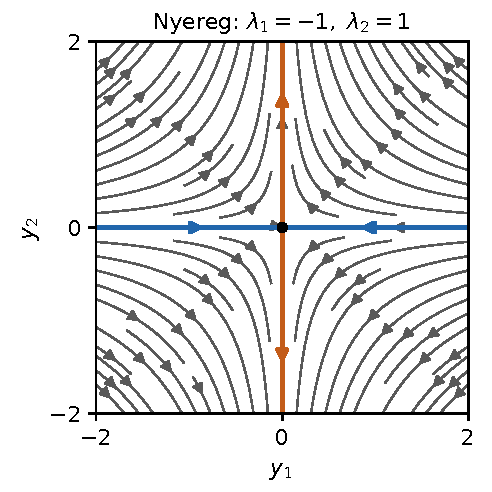
\includegraphics[width=.52\linewidth]{graphics_v3/phase_saddle.pdf}
\caption{Nyeregpont: $\lambda_1=-1$, $\lambda_2=1$. Kék egyenes: stabil irány; narancssárga egyenes: instabil irány. Az origó fekete pont.}\label{fig:phase_saddle}
\end{figure}

\paragraph*{Stabil és instabil csomópont.}
Az $A=\operatorname{diag}(-1,-2)$ mátrix esetén mindkét sajátérték negatív:
\[
y_1(t)=y_1(0)e^{-t},\qquad y_2(t)=y_2(0)e^{-2t}.
\]
Minden pálya az origóhoz tart. A második komponens gyorsabban csökken, ezért az általános pályák a lassabb, $y_1$ sajátirányhoz simulnak. Kivétel a tisztán gyors sajátirányon induló pálya. Az $A=\operatorname{diag}(1,2)$ rendszerben mindkét komponens növekszik: az origó instabil csomópont. A két ábra görbéi azonosak, az időirány ellentétes.
\begin{figure}[!htbp]\centering
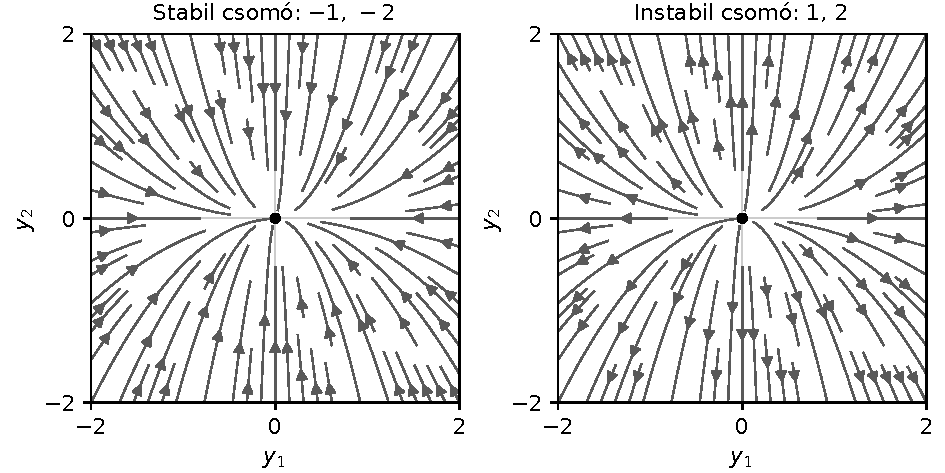
\includegraphics[width=\linewidth]{graphics_v3/phase_nodes.pdf}
\caption{Csomópontok. Balra $A=\operatorname{diag}(-1,-2)$: stabil; jobbra $A=\operatorname{diag}(1,2)$: instabil. A sajátirányokon egyenes, a többi kezdeti állapotból görbült pályát kapunk.}\label{fig:phase_nodes}
\end{figure}

\paragraph*{Stabil és instabil fókusz.}
Komplex konjugált sajátértékpárhoz valós koordinátákban a
\begin{equation}\label{eq:focus_block}
A=\begin{pmatrix}\alpha&-\beta\\\beta&\alpha\end{pmatrix},\qquad
\lambda_{1,2}=\alpha\pm i\beta,\quad \beta\neq0
\end{equation}
blokk tartozhat. A $y_1=\rho\cos\theta$, $y_2=\rho\sin\theta$ polárkoordinátákkal
\begin{equation}\label{eq:focus_polar}
\dot\rho=\alpha\rho,\qquad \dot\theta=\beta,\qquad
\rho(t)=\rho(0)e^{\alpha t}.
\end{equation}
A $\beta$ a forgást, $\alpha$ a spirál összehúzódását vagy tágulását szabályozza. $\alpha<0$ esetén stabil, $\alpha>0$ esetén instabil fókuszt kapunk. A \ref{fig:phase_foci}. ábrán $\beta=1$, ezért mindkét esetben az óramutató járásával ellentétes a forgás; csak a sugár időbeli változása különbözik.
\begin{figure}[!htbp]\centering
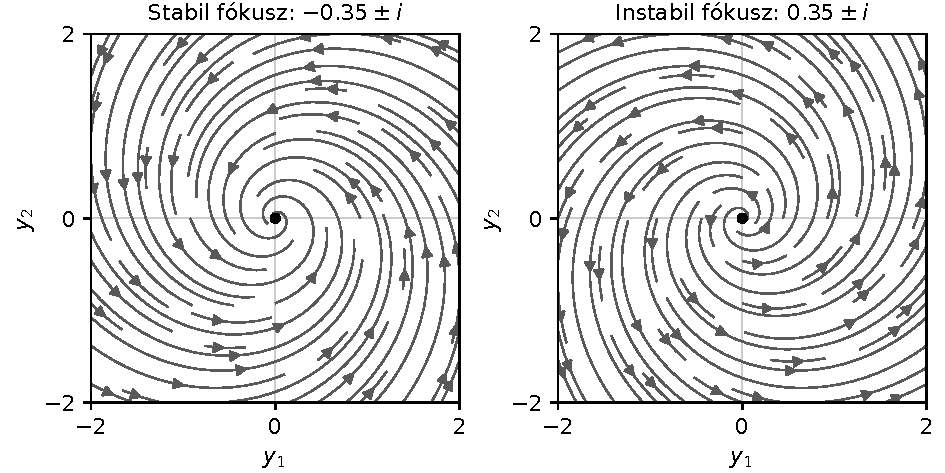
\includegraphics[width=\linewidth]{graphics_v3/phase_foci.pdf}
\caption{Fókuszok: $\lambda_{1,2}=-0{,}35\pm i$ (balra) és $\lambda_{1,2}=0{,}35\pm i$ (jobbra). A stabil fókusz pályái befelé, az instabiléi kifelé spiráloznak.}\label{fig:phase_foci}
\end{figure}

$\alpha=0$ esetén ebben a \emph{lineáris} rendszerben a sugár állandó: centrumot kapunk, amely stabil, de nem aszimptotikusan stabil. Egy nemlineáris rendszer tisztán képzetes sajátértékei azonban önmagukban nem garantálnak centrumot.

\paragraph*{Osztályozás nyom és determináns alapján.}
Valós $2\times2$ mátrixnál legyen $\tau=\operatorname{tr}A$, $\Delta=\det A$, $D=\tau^2-4\Delta$. A karakterisztikus egyenlet
\[
\lambda^2-\tau\lambda+\Delta=0
\]
alapján $\Delta<0$ nyerget, $\Delta>0$, $D>0$ csomópontot, $\Delta>0$, $D<0$, $\tau\neq0$ fókuszt jelent. Az utóbbi két eset stabil, ha $\tau<0$, és instabil, ha $\tau>0$. A $D=0$ ismétlődő, nemnulla sajátérték esetén a sajátvektorokat is vizsgáljuk: lehet csillagcsomó vagy egyetlen sajátirányú, degenerált csomó. $\Delta=0$ vagy $\tau=0$, $\Delta>0$ esetén nemhiperbolikus határesethez érünk.

A csomó és a fókusz geometriailag különbözik, de azonos stabilitás mellett topologikusan ekvivalens lehet. A topologikus ekvivalencia nem őrzi meg a szögeket, a görbületet vagy a spirálalakot. Hiperbolikus pontnál a nemlineáris és a linearizált rendszer lokális topologikus ekvivalenciáját a Hartman--Grobman-tétel biztosítja \cite[2.1.4. szakasz, 2.2. tétel]{dib}.

\FloatBarrier
\subsection{Az $N$ dimenziós rendszer linearizálása}
Legyen $x\in\mathbb R^N$, $f$ az $x^*$ környezetében legalább $C^1$, és $f(x^*)=0$. Vezessük be a $y=x-x^*$ eltérést. A Taylor-kifejtésből
\begin{equation}\label{eq:equilibrium_linearization_N}
\dot y=f(x^*+y)=Ay+R(y),\qquad
A=Df(x^*)=\left[\frac{\partial f_i}{\partial x_j}(x^*)\right]_{i,j=1}^{N},
\end{equation}
ahol $\|R(y)\|/\|y\|\to0$, ha $y\to0$. $f\in C^2$ esetén a maradék erősebb, $R(y)=O(\|y\|^2)$ becslést is kielégít. Az $A$ a \emph{Jacobi-mátrix}; a teljes linearizált vektormező $Ay$.

A maradéktagot elhagyva a konstans együtthatós
\begin{equation}\label{eq:linear_solution_N}
\dot y=Ay,\qquad y(t)=e^{At}y(0)
\end{equation}
rendszert kapjuk. Ez az egyensúly körüli közelítés, nem egy általános pálya körüli variációs egyenlet: ott a mátrix az időben változó referenciaállapot miatt $A(t)=Df(x(t))$. Az alapfelírást és a stabilitási kapcsolatot di Bernardo és szerzőtársai \cite[2.1.3--2.1.4. szakasz]{dib}, az általános hiperbolikus geometriát Kuznetsov \cite[2.2.1. szakasz]{kuznetsov_book} tárgyalja.

\subsection{Főtengelytranszformáció és modális koordináták}
\paragraph*{Diagonalizálható mátrix.}
Tegyük fel először, hogy $A$-nak van $N$ lineárisan független sajátvektora:
\[
Av_j=\lambda_jv_j,\qquad
S=[v_1\ \cdots\ v_N],\qquad
\Lambda=\operatorname{diag}(\lambda_1,\ldots,\lambda_N).
\]
Mivel $AS=S\Lambda$, a $y=Sz$ koordinátacsere után
\begin{equation}\label{eq:modal_transform}
S\dot z=ASz,\qquad
\dot z=S^{-1}ASz=\Lambda z.
\end{equation}
A modális egyenletek szétválnak:
\begin{equation}\label{eq:modal_solution}
\dot z_j=\lambda_jz_j,\qquad
z_j(t)=z_j(0)e^{\lambda_jt},\qquad
y(t)=\sum_{j=1}^{N}z_j(0)e^{\lambda_jt}v_j.
\end{equation}
Ez mutatja meg a sajátértékek szerepét: a sajátirányokhoz vagy invariáns síkokhoz tartozó amplitúdók növekedési ütemét adják. A báziscserét és a sajátértékeket Kuznetsov \cite[A.1.2--A.1.3. szakasz]{kuznetsov_book} foglalja össze.

A \emph{főtengelytranszformáció} elnevezést itt sajátvektor-bázisra való áttérésként használjuk. Általános, nem szimmetrikus Jacobi-mátrixnál $S$ nem feltétlenül ortogonális: a transzformáció nyírást és skálázást is tartalmazhat, és $S^{-1}\neq S^\mathsf T$. Valós szimmetrikus $A$ esetén választható ortonormált sajátvektor-bázis, ekkor valóban $S^{-1}=S^\mathsf T$. Egy általános dinamikai rendszerben a Jacobi-mátrix szimmetriáját nem tételezhetjük fel.

\exampleheading{Példa: nem merőleges sajátirányok.}
Legyen
\begin{equation}\label{eq:nonorthogonal_example}
A=\begin{pmatrix}-1&1\\0&-2\end{pmatrix},\qquad
S=\begin{pmatrix}1&-1\\0&1\end{pmatrix},\qquad
S^{-1}AS=\begin{pmatrix}-1&0\\0&-2\end{pmatrix}.
\end{equation}
A sajátvektorok $(1,0)^\mathsf T$ és $(-1,1)^\mathsf T$, amelyek nem merőlegesek. A $y=Sz$ átalakítás $y_1=z_1-z_2$, $y_2=z_2$, és az új egyenletek $\dot z_1=-z_1$, $\dot z_2=-2z_2$. A stabilitás nem változik a báziscserével, a pályák alakja viszont igen.
\exampleend

\paragraph*{Komplex sajátértékpár valós leírása.}
Valós $A$ esetén a nemvalós sajátértékek konjugált párokban jelennek meg. Ha $\lambda=\alpha+i\beta$ sajátvektora $v=p+iq$, akkor a $p,-q$ valós bázisban az adott invariáns sík mátrixa a \eqref{eq:focus_block} blokk. Így komplex koordináták használata nélkül is megkapjuk a forgást és az $e^{\alpha t}$ amplitúdóváltozást. A többi sajátirányhoz tartozó koordináták ettől függetlenül kezelhetők, ha az egész mátrix diagonalizálható a komplex számok felett.

\paragraph*{Ha nincs elegendő sajátvektor.}
Ismétlődő sajátérték nem feltétlenül jelent problémát, de előfordulhat, hogy $A$ nem diagonalizálható. Ilyenkor általánosított sajátvektorokkal Jordan-alakra térünk át, $S^{-1}AS=J$ \cite[A.1.4. szakasz, A.1. tétel]{kuznetsov_book}. Egy kétdimenziós Jordan-blokk például
\begin{equation}\label{eq:jordan_exponential}
J=\begin{pmatrix}\lambda&1\\0&\lambda\end{pmatrix},\qquad
e^{Jt}=e^{\lambda t}\begin{pmatrix}1&t\\0&1\end{pmatrix}.
\end{equation}
Nagyobb blokkoknál magasabb fokú időpolinomok is megjelennek. Ha $\operatorname{Re}\lambda<0$, az exponenciális lecsengés minden ilyen polinomot elnyom. Nulla valós résznél viszont a polinomiális tényező növekedést okozhat: a stabilitási határon a Jordan-szerkezetet is vizsgálni kell.

\subsection{Az egyensúly stabilitásának általános kritériuma}
\paragraph*{Mit értünk stabilitáson?}
Az $x^*$ egyensúly \emph{Ljapunov-stabil}, ha minden elegendően kis $\varepsilon>0$ számhoz található $\delta>0$, hogy
\begin{equation}\label{eq:lyapunov_stability_definition}
\|x(0)-x^*\|<\delta
\quad\Longrightarrow\quad
\|x(t)-x^*\|<\varepsilon\quad\text{minden }t\geq0\text{ esetén}.
\end{equation}
\emph{Lokálisan aszimptotikusan stabil}, ha emellett egy környezetéből induló minden megoldás $x^*$-hoz tart. \emph{Lokálisan exponenciálisan stabil}, ha valamely $C,\gamma>0$ mellett, elég kis kezdeti eltérésekre
\begin{equation}\label{eq:exponential_stability}
\|x(t)-x^*\|\leq Ce^{-\gamma t}\|x(0)-x^*\|.
\end{equation}
Az aszimptotikus stabilitás tehát többet állít a közelség megőrzésénél. A definíciókat lásd \cite[2.1.3. szakasz, 2.9--2.10. definíció]{dib} és \cite[1.3.3. szakasz]{kuznetsov_book}.

\paragraph*{Lineáris rendszer: teljes spektrális feltétel.}
A $\dot y=Ay$ origója pontosan akkor aszimptotikusan stabil, ha
\begin{equation}\label{eq:hurwitz_criterion}
\boxed{\operatorname{Re}\lambda_j(A)<0\qquad(j=1,\ldots,N).}
\end{equation}
Ekkor exponenciálisan is stabil; az ilyen mátrixot Hurwitz-mátrixnak nevezzük. A feltétel a nem diagonalizálható mátrixokra is igaz. A megoldás normája közben átmenetileg nőhet, különösen nem merőleges sajátirányok mellett; az exponenciális becslés $C$ szorzója ezért nem feltétlenül egy. Ha valamely sajátérték valós része pozitív, az origó instabil.

A lineáris rendszer \emph{Ljapunov-stabilitásának} szükséges és elégséges feltétele az, hogy minden sajátértékre $\operatorname{Re}\lambda_j\leq0$, és a képzetes tengelyen fekvő sajátértékekhez csak egydimenziós komplex Jordan-blokkok tartozzanak. Utóbbit semisimple sajátértéknek is mondjuk. Ilyen centrumirányok jelenlétében a megoldás korlátos maradhat, de általában nem tart az origóhoz. A $J=\left(\begin{smallmatrix}0&1\\0&0\end{smallmatrix}\right)$ ellenpélda: minden sajátértéke nulla, mégis $y_1(t)=y_1(0)+t\,y_2(0)$, ezért instabil.

\paragraph*{Nemlineáris rendszer: a linearizálás hatóköre.}
Az $f\in C^1$ rendszer $x^*$ egyensúlyánál, $A=Df(x^*)$ jelöléssel:
\begin{itemize}
\item Ha minden sajátérték valós része negatív, $x^*$ lokálisan exponenciálisan, így aszimptotikusan stabil.
\item Ha legalább egy sajátérték valós része pozitív, $x^*$ instabil, akkor is, ha más sajátértékek valós része nulla.
\item Ha nincs pozitív valós rész, de van nulla valós részű sajátérték, a linearizálás általában nem dönt a nemlineáris stabilitásról.
\end{itemize}
Az utolsó esetben nem szabad a lineáris centrum stabilitását automatikusan átvinni a nemlineáris rendszerre. Például a $\dot x=-x^3$ és a $\dot x=x^3$ egyenlet origójában ugyanaz az $A=0$ linearizálás, de az első egyensúly aszimptotikusan stabil, a második instabil. A negatív valós részű spektrum ezért elégséges, de nem szükséges feltétele a nemlineáris aszimptotikus stabilitásnak. A nemhiperbolikus esetekhez magasabb rendű tagok, középponti sokaság vagy Ljapunov-függvény vizsgálata szükséges; lásd \cite[5.1--5.2. szakasz]{kuznetsov_book}.

Ha egyik sajátérték valós része sem nulla, az egyensúly \emph{hiperbolikus}. A negatív és pozitív valós részű sajátértékek algebrai multiplicitással számított száma $N_s$, illetve $N_u$, és $N_s+N_u=N$. A lokális stabil és instabil sokaság dimenziója rendre $N_s$, illetve $N_u$; az egyensúlyban a megfelelő általánosított sajátalterek érintik őket. $N_s>0$, $N_u>0$ esetén $N$ dimenzióban is nyeregpontot kapunk \cite[2.2.1. szakasz, 2.1. tétel]{kuznetsov_book}.

\paragraph*{Ljapunov-függvény és a mátrixfeltétel kapcsolata.}
A spektrális eredmény energiaszerű becsléssel is értelmezhető. Hurwitz-mátrixhoz minden $Q=Q^\mathsf T>0$ mellett létezik egyértelmű $P=P^\mathsf T>0$, amelyre
\begin{equation}\label{eq:lyapunov_matrix}
A^\mathsf TP+PA=-Q.
\end{equation}
Ekkor $V(y)=y^\mathsf TPy$ pozitív definit, és a lineáris rendszerben $\dot V=-y^\mathsf TQy<0$ minden $y\neq0$ esetén. A nemlineáris rendszerben
\[
\dot V=-y^\mathsf TQy+2y^\mathsf TPR(y),
\]
és a maradék $o(\|y\|^2)$, ezért elegendően kis környezetben a negatív kvadratikus tag dominál. Ez a lokális stabilitást igazolja; a vonzási tartomány teljes méretét nem határozza meg.

Általánosabban, egy $C^1$, pozitív definit $V$ függvény és a pálya menti negatív definit $\dot V$ lokális aszimptotikus stabilitást biztosít; $\dot V\leq0$ önmagában rendszerint csak stabilitást igazol. A $\dot x=-x^3$ példában $V=x^2/2$, $\dot V=-x^4$, így a módszer a nulla sajátérték ellenére dönt. A szemléletet di Bernardo és szerzőtársai \cite[2.1.3. és 2.4.1. szakasz]{dib} kapcsolja a szakaszos rendszerek stabilitásvizsgálatához.

Végül a fenti Jacobi-kritérium \emph{sima környezetben fekvő} egyensúlyra vonatkozik. Kapcsolófelületen elhelyezkedő pontnál a két oldali mátrix külön vizsgálata általában nem elegendő; a sliding dinamikát, az átmeneti szabályokat vagy a boundary equilibrium geometriáját is figyelembe kell venni \cite[2.4.1. szakasz és 5. fejezet]{dib}.

\section{Stabilitásvesztési formák}
Az egyensúlyok sima bifurkációinak könyvbeli háttere: \cite[2.1.6. szakasz]{dib} és \cite[3.1--3.5. szakasz]{kuznetsov_book}.

A Hopf-bifurkáció részletes feltételeit \cite{kuznetsov} foglalja össze.

Sima, egyparaméteres síkbeli rendszerek egyensúlyainak generikus lokális bifurkációi közül két alapvető eset a saddle-node bifurcation és a Hopf-bifurkáció. Saddle-node bifurcation esetén egy egyszerű sajátérték nullává válik, és megfelelő nemelfajulási feltételek mellett két egyensúlyi ág találkozik és megszűnik, illetve keletkezik. Hopf-bifurkációnál egy komplex konjugált sajátértékpár $\lambda_{1,2}(\mu)=\alpha(\mu)\pm i\omega(\mu)$ halad át a képzetes tengelyen: $\alpha(\mu_0)=0$, $\omega(\mu_0)>0$ és $\alpha'(\mu_0)\neq0$. A generikus esethez az első Ljapunov-együttható nemnullasága is szükséges.

Szuperkritikus Hopf-bifurkációnál stabil, kis amplitúdójú határciklus születik; szubkritikus esetben a lokálisan megjelenő határciklus instabil. Az utóbbi esetben fellépő véges amplitúdójú ugrás és hiszterézis a további, globális dinamikától függ. Szimmetriák vagy más speciális feltételek mellett transcritical bifurcation és pitchfork bifurcation is előfordulhat.

\section{Periodikus pályák, monodrómia-mátrix}
A Poincaré-leképezéshez és a periodikus pálya stabilitásához lásd \cite[2.1.5. szakasz]{dib}, illetve \cite[1.5. és 2.2.3. szakasz]{kuznetsov_book}.


Tekintsük az $\dot{x}=f(x)$ dinamikai rendszer $x(t)=p(t)$ $T$ periódusú periodikus pályáját, azaz $p(t)=p(t+T)$. A pálya közelében szeretnénk a dinamikát vizsgálni, ezért megkonstruáljuk az ún. \emph{Poincaré-metszetet}, amely egy $n-1$ dimenziós $\Pi$ felület, amely tartalmazza az $x_p=p(t^*)$ pontot és transzverzálisan metszi a pályát (= nem érinti).

Legyen a Poincaré-metszetet definiáló felület: $\Pi = \{x\in\mathbb{R}^n:\pi(x)=0\}$! Ekkor a transzverzalitás feltétele, hogy Poincaré felületre merőleges vektornak ($\pi_x$) $x_p$-ben legyen a trajektória irányába eső vetülete, azaz $\pi_x(x_p) f(x_p)=<\pi_x(x_p), f(x_p)>\neq 0$.

A Poincaré leképezés ezek után, ha $x$ megfelelően közel van $x_p$-hez, a $P(x)=\Phi(x,\tau(x))$ alakban írható, ahol $\tau(x)$-et (a megzavart pálya visszatérési idejét) a $\pi(\Phi(x,\tau(x)))=0$ egyenlet definiálja. Itt $\tau(x)$ visszatérési idő; egy közeli, nemperiodikus pályának általában nincs periódusa.

A periodikus pálya stabilitását az ún. \emph{monodrómia-mátrix} kiszámításával lehet vizsgálni. Vizsgáljuk a
\begin{equation}
\dot{x}=A(t)x
\label{eq:per_lin}
\end{equation}
dinamikai rendszert, melyben $A(t)$ periodikus $T$ periódussal. Legyen $X(t)$ \eqref{eq:per_lin} fundamentális megoldásmátrixa, azaz $n$ darab lineárisan független megoldásból képzett mátrix. Ekkor létezik olyan \emph{konstans} $C$ mátrix, melyre $X(t+T)=X(t)C$. Továbbá, ennek kiszámítása egyszerű, hiszen $t=0$-ban $X(T)=X(0)C$, tehát $C=X^{-1}(0)X(T)$. Továbbá, ha $X(0)=I$, akkor $C=X(T)$. A $C$ mátrix a monodrómia reprezentációja az $X(0)$ bázisban; az állapotkoordinátákban a mátrix $X(T)X(0)^{-1}$. A két mátrix hasonló, ezért multiplikátoraik azonosak.

Így az eredeti $\dot{x}=f(x)$ dinamikai rendszer $p(t)$ periodikus pályája körül linearizálva kapjuk az $\dot y =f'(p(t))y$ variációs egyenletet, melynek a \emph{fundamentális megoldását} kell $t=T$ pillanatban kiszámítani, ahol $T$ a periódusidő. Ezt legegyszerűbben úgy tehetjük meg, ha speciális kezdeti feltételekből numerikusan integráljuk az egyenletet:
\[
\mathbf{M}=\begin{bmatrix}
\Phi_p(\mathbf{e}_1,T) & \cdots & \Phi_p(\mathbf{e}_n,T)
\end{bmatrix}
\]
ahol $\Phi_p$ a variáció egyenlet fundamentális megoldás operátora, $\mathbf{e}_i$ az i-edik egységvektor. Nemállandó autonóm periodikus pálya esetén az időeltolási irányhoz $1$ multiplikátor tartozik. Ha ez egyszeres, és minden további multiplikátorra $|\lambda_j|<1$, a pálya orbitálisan aszimptotikusan stabil. Ha valamelyikre $|\lambda_j|>1$, a pálya instabil; további egységkörön fekvő multiplikátorok esetén a linearizálás általában nem dönt. A Poincaré-leképezés deriváltja a transzverzális, nemtriviális multiplikátorokat tartalmazza.

A fundamentális megoldásmátrixot most $\Phi(t)$ jelöli; ekkor $\Phi(t+T)=\Phi(t)B$. A konstans $B\in\mathbb R^{n\times n}$ mátrix pontos definíciója a $t=0$ helyettesítésből:
\[
\Phi(T)=\Phi(0)B,\qquad
\boxed{B=\Phi(0)^{-1}\Phi(T)}.
\]
Ez az előbb $C$-vel jelölt mátrix, a választott fundamentális megoldás kezdőbázisában. Ha $\Phi(0)=I$, akkor
\[
B=\Phi(T)=\begin{bmatrix}y_1(T)&\cdots&y_n(T)\end{bmatrix}=\mathbf M,
\qquad \dot y_j=A(t)y_j,\quad y_j(0)=e_j.
\]
Tehát oszlopai az egységvektorokból indított variációs megoldások egy periódus utáni értékei. Általános kezdőbázisnál az állapotkoordinátákban vett monodrómia-mátrix $\mathbf M=\Phi(T)\Phi(0)^{-1}=\Phi(0)B\Phi(0)^{-1}$; normalizált kezdőbázisnál $B=\mathbf M$. A determinánst Liouville formulája adja:


\begin{equation}
\det(B)=\exp \left( \int_0^T \mathrm{tr}(A(s)) ds\right).
\end{equation}

\exampleheading{Példa: a fundamentális megoldásmátrix előállítása.}
Először egy egyszerű, csatolt lineáris rendszeren végezzük el az oszloponkénti konstrukciót. Dimenziótlan idővel és állapotokkal legyen
\begin{equation}\label{eq:fundamental_example_system}
 \dot y=Ay,\qquad
 A=\begin{pmatrix}-1&1\\0&-2\end{pmatrix},\qquad
 \begin{cases}\dot y_1=-y_1+y_2,\\\dot y_2=-2y_2.\end{cases}
\end{equation}
Ez két lecsengő folyamat egyszerű modellje: a második állapot gerjeszti az elsőt, visszahatás azonban nincs. A normalizált fundamentális megoldásmátrixot $X(t)$ jelöli; azt keressük, amelyre
\begin{equation}\label{eq:fundamental_example_ivp}
 \dot X(t)=AX(t),\qquad X(0)=I.
\end{equation}
A mátrix minden oszlopa ugyanannak a differenciálegyenletnek egy megoldása, de más kezdeti állapotból indul. Az oszlopokat $y^{(1)}$ és $y^{(2)}$ jelöli; a zárójeles felső index itt a megoldást sorszámozza, nem deriválást jelent.

Az első oszlophoz $y^{(1)}(0)=e_1=(1,0)^{\mathsf T}$ kezdeti állapotot választunk.
A második egyenletből $y_2^{(1)}(t)=0$. Ezt az elsőbe helyettesítve $\dot y_1^{(1)}=-y_1^{(1)}$, $y_1^{(1)}(0)=1$, tehát
\[
 y^{(1)}(t)=\begin{pmatrix}e^{-t}\\0\end{pmatrix}.
\]
A második oszlophoz $y^{(2)}(0)=e_2=(0,1)^{\mathsf T}$ kezdeti állapot tartozik.
Most $y_2^{(2)}(t)=e^{-2t}$. Az első komponens egyenlete és kezdeti feltétele
\[
 \dot y_1^{(2)}+y_1^{(2)}=e^{-2t},\qquad y_1^{(2)}(0)=0.
\]
Az $e^t$ integráló tényezővel szorozva, majd $0$ és $t$ között integrálva
\[
 \frac{d}{dt}\bigl(e^t y_1^{(2)}(t)\bigr)=e^{-t},\qquad
 e^t y_1^{(2)}(t)=\int_0^t e^{-s}\,ds=1-e^{-t}.
\]
Így $y_1^{(2)}(t)=e^{-t}-e^{-2t}$, és
\[
 y^{(2)}(t)=\begin{pmatrix}e^{-t}-e^{-2t}\\e^{-2t}\end{pmatrix}.
\]

\begin{equation}\label{eq:fundamental_example_matrix}
 \boxed{X(t)=\begin{bmatrix}y^{(1)}(t)&y^{(2)}(t)\end{bmatrix}
 =\begin{pmatrix}e^{-t}&e^{-t}-e^{-2t}\\0&e^{-2t}\end{pmatrix}.}
\end{equation}
Közvetlenül látható, hogy $X(0)=I$. A differenciálegyenlet ellenőrzése is egyszerű:
\[
 \dot X(t)=\begin{pmatrix}-e^{-t}&-e^{-t}+2e^{-2t}\\0&-2e^{-2t}\end{pmatrix}
 =AX(t).
\]
Továbbá $\det X(t)=e^{-3t}\neq0$ minden véges $t$ esetén, ezért az oszlopok lineárisan függetlenek: valóban fundamentális megoldásmátrixot kaptunk. A determináns megegyezik a Liouville-formula eredményével, hiszen $\operatorname{tr}A=-3$.


Ha $y(0)=(a,b)^{\mathsf T}$, a linearitás miatt
\begin{equation}\label{eq:fundamental_example_solution}
 y(t)=X(t)y(0)=a\,y^{(1)}(t)+b\,y^{(2)}(t)
 =\begin{pmatrix}a e^{-t}+b(e^{-t}-e^{-2t})\\b e^{-2t}\end{pmatrix}.
\end{equation}
Az $X_{12}(t)$ elem tehát azt mutatja meg, hogyan hat a második állapot kezdeti eltérése az első állapot későbbi értékére. A kezdeti egységmátrix oszlopai nem maradnak állandók: mindegyiket a dinamika szerint továbbvezetjük. Mivel itt $A$ állandó, $X(t)=e^{At}$ is írható; a fenti számítás ezt a mátrixexponenciálist állította elő.


A konstans $A$ bármely $T>0$ választással periodikus együtthatómátrixnak tekinthető. Egy ilyen rögzített időszakaszra $\mathbf M=X(T)$, sajátértékei $e^{-T}$ és $e^{-2T}$. Ebben a példában azonban egy stabil egyensúly körüli rendszert vizsgálunk, nem egy nemállandó autonóm periodikus pálya variációs egyenletét. Ezért nincs kötelező, időeltoláshoz tartozó egységnyi multiplikátor. A következő példa már egy határciklushoz tartozó fundamentális megoldásmátrixot és monodrómia-mátrixot mutat be.
\exampleend

\exampleheading{Példa: határciklus fundamentális megoldásmátrixa.} Tekintsük a következő rendszert: $\dot{r}=r (1-r^2)$ és $\dot{\phi} = 1$. A határciklus polárkoordinátákban $r(t)=1$, $\phi(t)=t$ (modulo $2\pi$), vagyis az $(x,y)$ koordináta-rendszerben $p(t) = \{(x,y)=(\cos t,\sin t):t\in\mathbb{R}\}$.

A radiális perturbáció legyen $\rho=r-1$. Linearizálva $\dot{\rho}=-2\rho$, ezért a radiális eltérések lecsengenek. A fázisirány semleges; a stabilitás orbitális értelemben értendő.

A pálya vizsgálatához térjünk át derékszögű koordináta rendszerre!

\begin{align}
x=r\cos \phi& \quad \rightarrow \quad & \dot{x}=\dot{r} \cos \phi-r \sin\phi\, \dot{\phi}=x\left(1-x^2-y^2\right)-y\\
y=r\sin \phi& \quad \rightarrow \quad & \dot{y}=\dot{r} \sin \phi+r \cos\phi\, \dot{\phi}=y\left(1-x^2-y^2\right)+x
\end{align}

Itt kihasználtuk, hogy pl. $\dot{r}\cos \phi=r\cos\phi(1-r^2)=x(1-(x^2+y^2))$ ill. $\dot{\phi}=1$. A fenti dinamikai rendszer  általános linearizáltja és annak periodikus pálya közelében vett alakja:
\begin{equation}
f'(p(t)) = \left. \begin{pmatrix}
1-3x^2-y^2 & -1-2xy \\
1-2xy & 1-x^2-3y^2 \\
\end{pmatrix} \right|_{p(t)}=
\begin{pmatrix}
-2\cos^2t & -1-\sin 2t \\
1-\sin 2t & -2\sin^2t \\
\end{pmatrix}
\end{equation}

Így a perturbációs egyenlet

\begin{equation}
\dot{z}=\begin{pmatrix}
-2\cos^2t & -1-\sin 2t \\
1-\sin 2t & -2\sin^2t \\
\end{pmatrix} z
\end{equation}

A monodrómia-mátrix determinánsát analitikusan is ki tudjuk számítani:

\begin{align}
\det(B)&=\exp \left( \int_0^T \mathrm{tr}(A(t)) dt\right)=\exp \left( \int_0^T -2\cos^2t-2\sin^2t dt\right)\\
&=\exp \left( \int_0^T -2 dt\right)=e^{-4\pi}<1.
\end{align}

A determináns természetesen a sajátértékek (karakterisztikus multiplikátorok) szorzata, ám (periodikus pályáról lévén szó) az egyik sajátérték biztosan 1, mivel pedig itt kétdimenziós rendszerről van szó, a második pontosan a fenti eredmény. A $p(0)=(1,0)$ kezdőpontnál a monodrómia-mátrix pontos alakja (amelyet a numerikus integrálás közelít):

\begin{equation}
\mathbf{M}=\begin{pmatrix}
e^{-4\pi} & 0\\ 0 & 1\\
\end{pmatrix}.
\end{equation}

Mivel $e^{-4\pi}<1$, $p(t)$ pálya orbitálisan aszimptotikusan stabil. A függelékben közölt MATLAB-kód a variációs egyenletet integrálja, és a kapott mátrixot a pontos $\operatorname{diag}(e^{-4\pi},1)$ mátrixszal ellenőrzi. Az egységnyi multiplikátort a numerikus hiba erejéig kell visszakapnunk.

\phantomsection\label{use:monodromy}A teljes MATLAB-program az A függelék \ref{ap:monodromy}. szakaszában található (\pageref{ap:monodromy}. oldal).
\exampleend

\exampleheading{Példa: periodikus együtthatómátrix.\footnote{E. Folkers: Floquet’s Theorem, Bachelor’s Project Mathematics, University of Groningen}} Tekintsük a következő rendszert:
\begin{equation}
\dot{x}=A(t)x=\begin{pmatrix}
-1 & 1\\
0 & 1+ \cos t-\frac{\sin t}{2+\cos t}
\end{pmatrix}x.
\end{equation}

(Ebben az esetben \emph{nem} egy autonóm rendszer periodikus pályája körüli linearizált rendszert vizsgálunk, hanem egy általános lineáris rendszert periodikus együtthatómátrixszal: $A(t)=A(t+2\pi)$.) A rendszer megoldása:
\begin{align}
x_1(t)&=c_2 e^{t+\sin t}+c_3 e^{-t}\\
x_2(t)&=c_2e^{t+\sin t}\left( 2+\cos t\right).
\end{align}

A két független megoldást oszlopokba rendezve egy fundamentális mátrix:
\begin{equation}
X(t)=
\begin{pmatrix}
e^{t+\sin t} &  e^{-t}\\
e^{t+\sin t}\left( 2+\cos t\right) &0
\end{pmatrix},
\end{equation}

mivel az általános megoldás $x(t)=c_2 X_1(t)+c_3 X_2(t)$ alakban írható, ahol $X_i$ a fundamentális mátrix $i$-edik oszlopát jelenti. A monodrómia-mátrix:
\begin{align}
C&=X^{-1}(0)X(2\pi)\\
&=\begin{pmatrix}0&1/3\\1&-1/3\end{pmatrix}
\begin{pmatrix}e^{2\pi}&e^{-2\pi}\\3e^{2\pi}&0\end{pmatrix}
=\begin{pmatrix}e^{2\pi}&0\\0&e^{-2\pi}\end{pmatrix}.
\end{align}
A multiplikátorok $\lambda_1=e^{2\pi}\approx535{,}492$ és $\lambda_2=e^{-2\pi}\approx0{,}00186744$, ezért a zérusmegoldás instabil. Itt általános periodikus lineáris rendszerről van szó, így nem szükséges, hogy legyen egységnyi multiplikátor.
\exampleend

\section{Bifurkációk}

\subsection{Egyensúlyi helyzetek bifurkációi}\label{sec:eq_bif_types}
Az alábbi lista sima, egyparaméteres rendszerek helyi bifurkációit foglalja össze. Legyen $A=f_x(x^*,\mu)$, a kritikus paraméter az átskálázás után $\mu=0$. A megadott egyszerű normálalakok a kritikus irányok dinamikáját szemléltetik; az ábrák stabilitásjelöléseihez a többi sajátérték valós részét negatívnak feltételezzük. A kritikus sajátértékfeltétel önmagában nem elegendő: a paraméterfüggés és a vezető nemlineáris tag sem lehet elfajuló. Háttér: \cite[2.1.6. szakasz]{dib}, \cite[3. fejezet]{kuznetsov_book}.
\begin{itemize}
\item \textbf{Saddle-node bifurcation.} Egy stabil és egy instabil egyensúly találkozik és eltűnik, illetve keletkezik. \textit{Feltétel:} egy egyszerű $\lambda=0$ sajátérték; a redukált $\dot u=g(u,\mu)$ egyenletben $g_\mu\neq0$, $g_{uu}\neq0$. Példa: $\dot u=\mu-u^2$; $\mu>0$ esetén $u^*=\pm\sqrt\mu$.
\item \textbf{Transcritical bifurcation.} Két fennmaradó egyensúlyi ág keresztezi egymást és stabilitást cserél. \textit{Feltétel:} egyszerű $\lambda=0$, továbbá a két ág fennmaradását biztosító struktúra. Az egyik ágat $u=0$-ra helyezve $g(0,\mu)=0$, $g_{u\mu}\neq0$, $g_{uu}\neq0$. Példa: $\dot u=\mu u-u^2$, ágai $u^*=0$ és $u^*=\mu$.
\item \textbf{Pitchfork bifurcation.} Egy egyensúlyi ágból két szimmetrikus ág válik ki. \textit{Feltétel:} egyszerű $\lambda=0$, az $u\mapsto-u$ szimmetriát biztosító struktúra, $g_{u\mu}\neq0$, $g_{uuu}\neq0$. \textit{Supercritical} esetben $\dot u=\mu u-u^3$: $\mu>0$ mellett két stabil ág születik. \textit{Subcritical} esetben $\dot u=\mu u+u^3$: $\mu<0$ mellett két instabil mellékág van.
\item \textbf{Hopf-bifurkáció.} Az egyensúly körül kis amplitúdójú periodikus pálya jelenik meg vagy tűnik el. \textit{Feltétel:} egy egyszerű $\lambda_{1,2}=\pm i\omega_0$ pár, $\omega_0>0$, $d\operatorname{Re}\lambda/d\mu\neq0$, és nemnulla első Ljapunov-együttható. A $\dot r=\mu r-r^3$, $\dot\theta=\omega_0$ normálalak \textit{supercritical}: a stabil ciklus amplitúdója $r=\sqrt\mu$. A $\dot r=\mu r+r^3$ \textit{subcritical}: az instabil ciklus $r=\sqrt{-\mu}$, $\mu<0$. A negatív $r$ értékek nem fizikai amplitúdók.
\end{itemize}
A transcritical és a pitchfork bifurcation általában nem marad fenn tetszőleges, a struktúrát megsértő perturbáció mellett. A Hopf-bifurkációt az egyensúly bifurkációi közé soroljuk, mert a kritikus objektum az egyensúly, még ha a megjelenő objektum periodikus pálya is.
\begin{figure}[!htbp]\centering
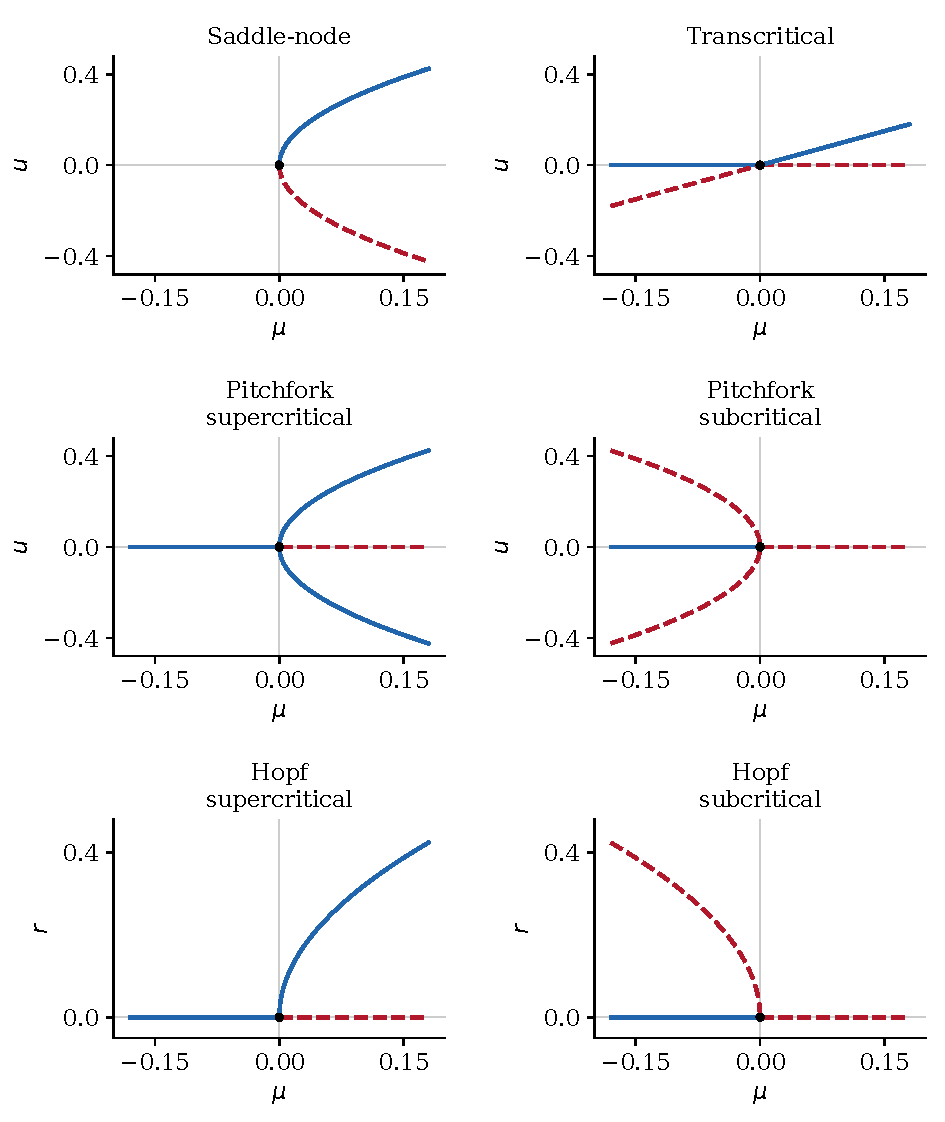
\includegraphics{graphics_v3/equilibrium_bifurcations.pdf}
\caption{Egyensúlyi bifurkációk normálalakjainak ágdiagramjai. Kék folytonos: stabil; piros szaggatott: instabil ág. Az első négy panelen $u^*$ egyensúlyi koordináta, az utolsó kettőn $r$ amplitúdó szerepel: ott $r=0$ az egyensúly, $r>0$ periodikus pálya. A fekete pont a kritikus állapot.}\label{fig:eq_bif_types}
\end{figure}
\FloatBarrier

\subsection{Periodikus pályák bifurkációi}\label{sec:cycle_bif_types}
Egy periodikus pályát a Poincaré-leképezés fixpontjaként vizsgálunk. Az alábbi $\rho$ értékek a transzverzális Floquet-multiplikátorok, vagyis $D P$ sajátértékei. Autonóm rendszerben a pálya menti időeltolás triviális $+1$ multiplikátorát előbb elhagyjuk. A többi, nemkritikus multiplikátor az ábrákon az egységkör belsejében van. Egy $m$ ciklusnál $D(P^m)$ vizsgálandó. Háttér: \cite[2.1.5--2.1.6. szakasz]{dib}, \cite[4--5. fejezet]{kuznetsov_book}.
\begin{itemize}
\item \textbf{Fold of cycles (saddle-node bifurcation of cycles).} Egy stabil és egy instabil periodikus pálya találkozik és eltűnik. \textit{Feltétel:} egyszerű, nemtriviális $\rho=+1$. A redukált leképezés $G(u,\mu)=P(u,\mu)-u$ maradékára $G_\mu\neq0$, $G_{uu}\neq0$. Szemléltető alak: $P(u,\mu)=u+\mu-u^2$.
\item \textbf{Period-doubling bifurcation.} A $T$ periódusú pálya stabilitást veszít, és egy hozzá közeli, közel $2T$ periódusú pálya jelenik meg. \textit{Feltétel:} egyszerű $\rho=-1$, $d\rho/d\mu\neq0$, és nemnulla redukált köbös együttható. A $P(u,\mu)=-(1+\mu)u+u^3$ \textit{supercritical} példa: a stabil kétciklus pontjai $u=\pm\sqrt\mu$. A köbös tag negatív előjelével a \textit{subcritical} esetben instabil kétciklus van $\mu<0$ mellett. Az ábra ugyanannak a megkettőzött pályának két metszéspontját mutatja.
\item \textbf{Neimark--Sacker-bifurkáció (torus bifurcation).} A Poincaré-leképezésben invariáns zárt görbe, a folytonos rendszerben invariáns tórusz jelenik meg a ciklus körül. \textit{Feltétel:} egyszerű $\rho_{1,2}=e^{\pm i\theta_0}$ pár, $d|\rho|/d\mu\neq0$, nemnulla első Ljapunov-együttható és $e^{ik\theta_0}\neq1$ ($k=1,2,3,4$). A radiális normálalak $r_{n+1}=(1+\mu)r_n-r_n^3$ \textit{supercritical}; a pozitív köbös tag \textit{subcritical} esetet ad. A tóruszon a mozgás nemrezonáns esetben kváziperiodikus, rezonanciánál periodikus mozgás is lehetséges. Autonóm folytonos rendszerben ehhez legalább három állapotváltozó kell.
\item \textbf{Transcritical bifurcation of cycles.} Két periodikus pálya ága keresztezi egymást és stabilitást cserél. \textit{Feltétel:} egyszerű, nemtriviális $\rho=+1$, a két ág fennmaradását biztosító struktúra; $G(0,\mu)=0$, $G_{u\mu}\neq0$, $G_{uu}\neq0$. Példa: $P(u,\mu)=u+\mu u-u^2$.
\item \textbf{Pitchfork bifurcation of cycles.} Egy szimmetrikus ciklusból két, egymás szimmetrikus képét adó ciklus válik ki. \textit{Feltétel:} egyszerű, nemtriviális $\rho=+1$, megfelelő szimmetria, $G_{u\mu}\neq0$, $G_{uuu}\neq0$. A $P(u,\mu)=u+\mu u-u^3$ \textit{supercritical}; pozitív köbös taggal \textit{subcritical}. A két mellékág itt két külön periodikus pálya, nem ugyanannak a kétciklusnak két pontja.
\end{itemize}
A normálalakok és stabilitásjelölések a kritikus pont kis környezetére vonatkoznak. A lista a sima helyi bifurkációkat foglalja össze; a globális homoclinic és heteroclinic eseményekre nincs önmagában elegendő helyi multiplikátorfeltétel. A piecewise-smooth rendszerek grazing, border-collision és sliding eseteit a későbbi fejezetek tárgyalják.
\begin{figure}[!htbp]\centering
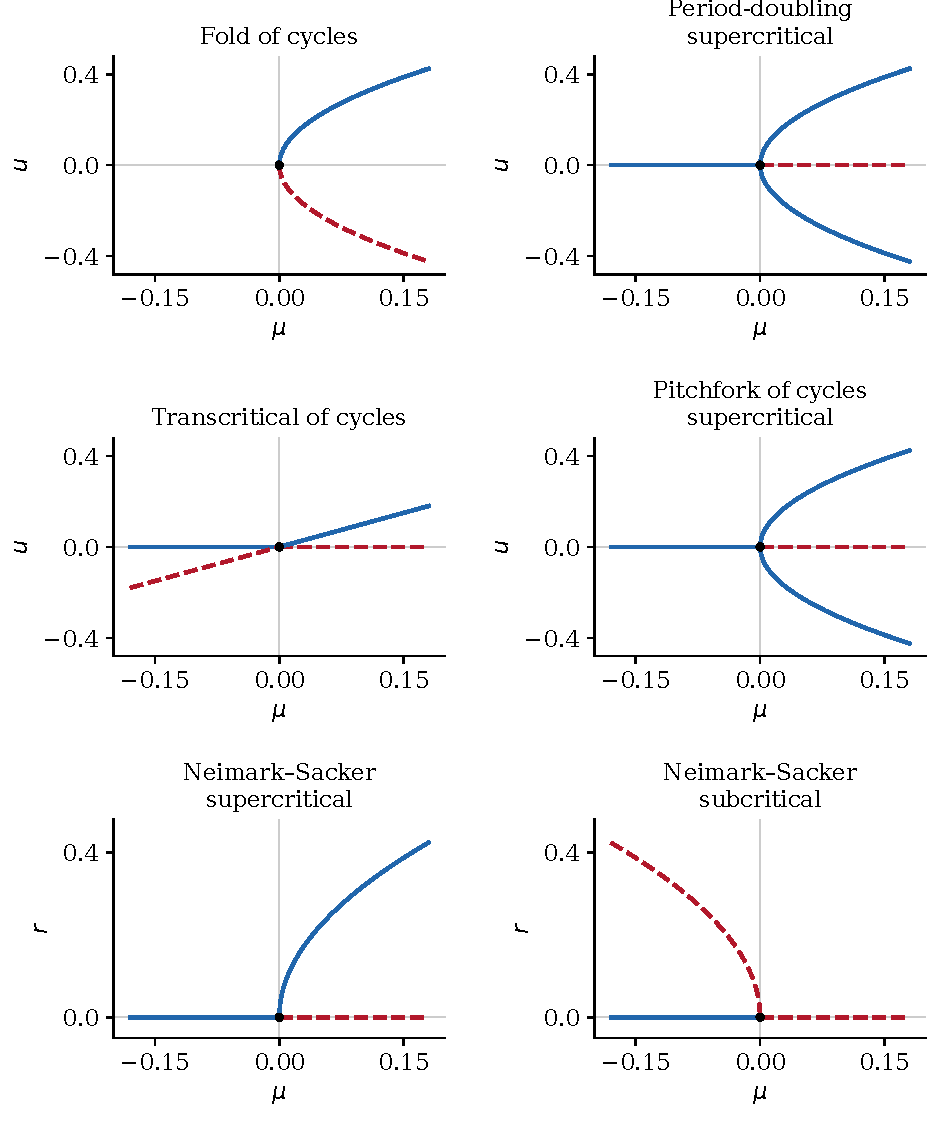
\includegraphics{graphics_v3/cycle_bifurcations.pdf}
\caption{Periodikus pályák helyi bifurkációi a Poincaré-metszeten. Kék folytonos: stabil; piros szaggatott: instabil. Az $u$ tengely a referenciaciklustól mért metszeti koordináta, nem a fizikai rezgésamplitúdó. A period-doubling panel két mellékága ugyanazon pálya két pontja, a pitchfork panel két mellékága két külön ciklus. A Neimark--Sacker-paneleken $r=0$ a kiinduló ciklus, $r>0$ az invariáns görbe sugara. A normálalakok helyi ágait ábrázoljuk.}\label{fig:cycle_bif_types}
\end{figure}
\FloatBarrier

\subsection{Szakadások osztályozása}\label{sec:discontinuity_types}
A szakaszos modelleknél először azt kell tisztázni, \emph{melyik mennyiség} folytonosságát vizsgáljuk: az erőt, a vektormezőt, annak deriváltját vagy magát az állapotot. Ezek eltérő tulajdonságok. Egy relé kapcsolásakor például az erő ugrik, miközben véges tömeg esetén a helyzet és a sebesség folytonos maradhat. Egy ideális merev ütközésnél viszont a sebesség ugrik.

Legyen $f$ egy $x_0$ környezetében, esetleg az $x_0$ pont kivételével értelmezett skalárfüggvény. Jelölje
\[
L_-=\lim_{x\to x_0^-}f(x),\qquad L_+=\lim_{x\to x_0^+}f(x)
\]
a két egyoldali határértéket. Folytonossághoz mindkettőnek léteznie kell, végesnek és egyenlőnek kell lenniük, továbbá $f(x_0)=L_-=L_+$ szükséges. Ha $f(x_0)$ nincs megadva, folytonos kiterjeszthetőségről beszélünk. Az alábbi osztályozásban az elsőfajú esetekhez mindkét véges egyoldali határérték létezését megköveteljük; minden más szakadást másodfajúnak nevezünk.

\paragraph{1. Megszüntethető szakadás: egy hibás vagy hiányzó pontérték.}
Ha $L_-=L_+=L\in\mathbb R$, de a pontérték hiányzik vagy $f(x_0)\neq L$, akkor az $f(x_0):=L$ hozzárendelés folytonossá teszi a függvényt. A görbe két oldala tehát illeszkedik; csak egy pontot kell helyesen kitölteni.

\exampleheading{Mérnöki példa: mozgóátlagoló szűrő zérus frekvencián.} Egy $\tau>0$ hosszúságú, középre igazított időablakon átlagoló szűrő frekvenciaválasza
\[
G(\omega)=\frac{\sin(\omega\tau/2)}{\omega\tau/2},\qquad \omega\neq0.
\]
A közvetlen képlet $\omega=0$-nál $0/0$ alakú, de a $\sin z=z+\mathcal O(z^3)$ sorfejtésből
\[
\lim_{\omega\to0}G(\omega)=1.
\]
A helyes kiterjesztés $G(0)=1$: egy állandó jelet az átlagolás változatlanul hagy. Ha egy program itt nullát ír be, mesterséges, megszüntethető szakadást hoz létre. Ezt a pontérték javításával kezeljük; nincs szükség kapcsolási vagy ütközési modellre.
\exampleend

\paragraph{2. Véges ugrás: a két oldal különböző értékhez tart.}
Ha $L_-,L_+\in\mathbb R$, de $L_-\neq L_+$, akkor ugrásszakadásról beszélünk. Az előjeles ugrás $[f]_{x_0}=L_+-L_-$, a nagysága $|L_+-L_-|$. Egyetlen pontérték megválasztásával az ugrás nem szüntethető meg.

\exampleheading{Mérnöki példa: ideális relés erőszabályozás.} Egy beavatkozó a mért $e$ hibajel előjelétől függően két erőszint között vált:
\[
f(e)=\begin{cases}-F_0,&e<0,\\+F_0,&e>0,\end{cases}
\qquad F_0>0.
\]
Ekkor $L_-=-F_0$, $L_+=F_0$, az ugrás $2F_0$. A $f(0)=0$ megállapodás sem teszi folytonossá a karakterisztikát. Ha az erő egy $m$ tömeget mozgat, $m\ddot q=f(e)$, akkor kapcsoláskor a gyorsulás ugrása $2F_0/m$ lehet, de a véges erőugrás nem okoz pillanatszerű sebességugrást: a gyorsulás időintegrálja folytonos sebességet ad.

Ugyanez a típus jelenik meg a kinetikus Coulomb-súrlódás $f(w)=-F_k\operatorname{sign}(w)$ törvényében, ahol $w$ a relatív sebesség. Itt $L_-=F_k$ és $L_+=-F_k$. A $w=0$-nál fennálló tapadást azonban általában nem egy önkényes pontérték, hanem egy erőintervallum és egy megfelelő tapadási szabály írja le. Ez vezet a \ref{sec:stick_slip}. szakasz többmódusú leírásához.
\exampleend

\paragraph{3. Másodfajú szakadás: nincs két véges egyoldali határérték.}
Két fontos lehetőséget érdemes megkülönböztetni: a függvény korlátlanná válhat, vagy véges értékek között oszcillálhat úgy, hogy nincs határértéke.

\exampleheading{Mérnöki példa korlátlan viselkedésre: csillapítatlan rezonancia.} A
\[
m\ddot q+kq=F_0\cos(\omega t),\qquad m,k>0
\]
egyenlet nem rezonáns harmonikus partikuláris megoldása $q_p(t)=C(\omega)\cos(\omega t)$, ahol
\[
C(\omega)=\frac{F_0}{k-m\omega^2},\qquad
\omega\neq\omega_0:=\sqrt{k/m}.
\]
$F_0>0$ mellett $C(\omega)\to+\infty$ balról és $C(\omega)\to-\infty$ jobbról. Ez a frekvenciaválasz pólusa, nem véges ugrás és nem megszüntethető hiányosság. A $C(\omega_0)=0$ beírása fizikailag hibás lenne: rezonancián nincs ilyen korlátos harmonikus partikuláris megoldás. Helyette például
\[
q_p(t)=\frac{F_0}{2m\omega_0}\,t\sin(\omega_0t)
\]
lineárisan növekvő burkolójú megoldást kapunk. Pozitív viszkózus csillapítással a kényszerrezgés amplitúdója
\[
A(\omega)=\frac{F_0}{\sqrt{(k-m\omega^2)^2+(c\omega)^2}},\qquad c>0,
\]
és a rezonancia közelében is véges. Ez jól mutatja, hogy a szingularitás az idealizált modellhez tartozik; a csillapítás bevezetése a modellt módosítja.
\exampleend

\exampleheading{Jelfeldolgozási ellenpélda: végtelenül gyorsuló frekvenciasöprés.} A mesterséges tesztjel
\[
u(t)=U_0\sin\!\left(\frac{\tau_0}{t_0-t}\right),\qquad t<t_0,
\quad U_0,\tau_0>0,
\]
korlátos, mégsem létezik bal oldali határértéke $t_0$-ban: egyre gyorsabban vesz fel $-U_0$ és $U_0$ közötti értékeket. A pillanatnyi körfrekvencia $\tau_0/(t_0-t)^2$ korlátlanul nő. Ez matematikai idealizáció, nem véges sávszélességű beavatkozó reális jele. Például mintavételező algoritmusok tesztelésénél szemléltetheti, miért nem következtethetünk néhány egymáshoz közeli mintából határérték létezésére. A $t_0$-beli pontérték pótlása itt sem segít.
\exampleend

\paragraph{4. Folytonos, de nem differenciálható karakterisztika.}
Ez \emph{nem a függvény szakadása}. A két oldal ugyanahhoz az értékhez tart, de a meredekség ugrik. A piecewise-smooth mechanikai modellekben ez különösen gyakori.

\exampleheading{Mérnöki példa: kétféle merevségű rugó.} A visszatérítő erő
\[
f(x)=\begin{cases}-k_-x,&x<0,\\0,&x=0,\\-k_+x,&x>0,\end{cases}
\qquad k_-,k_+>0,\quad k_-\neq k_+.
\]
Mindkét oldali erőhatárérték nulla, tehát $f$ folytonos. A két oldali derivált viszont $-k_-$ és $-k_+$, ezért $f'(0)$ nem létezik. Az $m\ddot x=f(x)$ rendszerben a helyzet, a sebesség és a gyorsulás is folytonos a határ átlépésekor, miközben a vektormező Jacobi-mátrixa vált. Itt a szegmensek folytonos illesztése szükséges; sebességugrást előíró reset leképezést alkalmazni hibás lenne. Ezt a modellt az \eqref{eq:bilinear_oscillator} egyenlet és a \ref{fig:bilinear_bvp}. ábra részletezi.
\exampleend

\paragraph{5. Állapotugrás: ideális merev ütközés.}
Ütközéskor a helyzet folytonos, de a sebességre
\[
q(t_0^+)=q(t_0^-),\qquad
v(t_0^+)=-r\,v(t_0^-),\qquad 0\leq r\leq1
\]
reset törvényt írunk elő. Ha $v(t_0^-)\neq0$, a sebesség időfüggvényének véges ugrása van: $[v]_{t_0}=-(1+r)v(t_0^-)$. Ez az impulzusszerű kontaktus idealizációja, nem egy korlátos erő egyszerű ugrása. A pozíció-idő görbe folytonos marad, de a meredeksége megtörik; az állapottérben reset leképezés kapcsolja össze az esemény előtti és utáni állapotot. A \ref{sec:square_root}. fejezet ezt az ütköző oszcillátoron mutatja be.

Többdimenziós rendszerben a kapcsolási határt $H(x)=0$ írja le; a két oldal a $H>0$ és $H<0$ tartomány. A megfelelő oldali határértékeket az adott felületponthoz közeledve vizsgáljuk. Ha a két vektormező határértéke eltér, diszkontinuus mezőről beszélünk; ha megegyezik, de a Jacobi-mátrixuk különbözik, a mező folytonos, csak nem sima. A reset leképezés pedig külön hibrid eseménytörvény. Az osztályozás tehát a modell és a számítási eljárás megválasztását is segíti, de önmagában nem jelent bifurkációt: ahhoz a dinamika kvalitatív változását kell kimutatni.

\chapter{\label{sec:filippov}Filippov-rendszerek}
A fejezet alapfogalmait di Bernardo és szerzőtársai \cite[2.2.3. szakasz]{dib} vezeti be; a relés szabályozás motivációját az 1.3.1. szakasz, a sliding bifurcations eseteit a 8. fejezet tárgyalja.


Tekintsük a
\begin{equation}
\dot{x}=\left\{
\begin{matrix}
F_1(x), \, \mathrm{ha} & H(x) > 0\\
F_2(x), \, \mathrm{ha} & H(x) < 0
\end{matrix}
\right.
\end{equation}
\noindent dinamikai rendszert. Feltesszük, hogy
$\left.F_1\right|_{H(x)=0} \neq \left.F_2\right|_{H(x)=0}$,
azaz a két vektormező határértéke eltér a felületen. Ez nem feltétlenül jelent különböző irányt. A
\begin{equation}
\Sigma=\{x:H(x)=0\}
\end{equation}
\noindent halmaz az úgynevezett \emph{kapcsolófelület}  (\textit{switching manifold}). Kapcsolófelületre mutat példát a \ref{fig:kapcsolofelulet}.~ábrán látható fekete szaggatott vonal.

A kör alakú határhoz most konkrét, dimenziótlan példát adunk. Legyen $x=(x_1,x_2)^\mathsf T$, és
\begin{equation}\label{eq:circle_switch_H}
H(x)=1-x_1^2-x_2^2.
\end{equation}
Így $\Sigma$ az egységkör, $H>0$ a kör belseje, $H<0$ a külseje. A két vektormező legyen
\begin{equation}\label{eq:circle_switch_fields}
F_1(x)=\begin{pmatrix}x_1\\-x_2\end{pmatrix}\quad(H>0),\qquad
F_2(x)=\begin{pmatrix}1\\-x_1\end{pmatrix}\quad(H<0).
\end{equation}
Belül tehát $\dot x_1=x_1$, $\dot x_2=-x_2$ nyeregtípusú mozgás, kívül $\dot x_1=1$, $\dot x_2=-x_1$ áramlás érvényes. A körön a két mező határértékei különböznek; az ottani folytatás szabályát a következőkben bevezetett Filippov-konstrukció adja meg. A \ref{fig:kapcsolofelulet}. ábrát közvetlenül ezekből a képletekből számítottuk újra.

\begin{figure}[htbp]
\centering
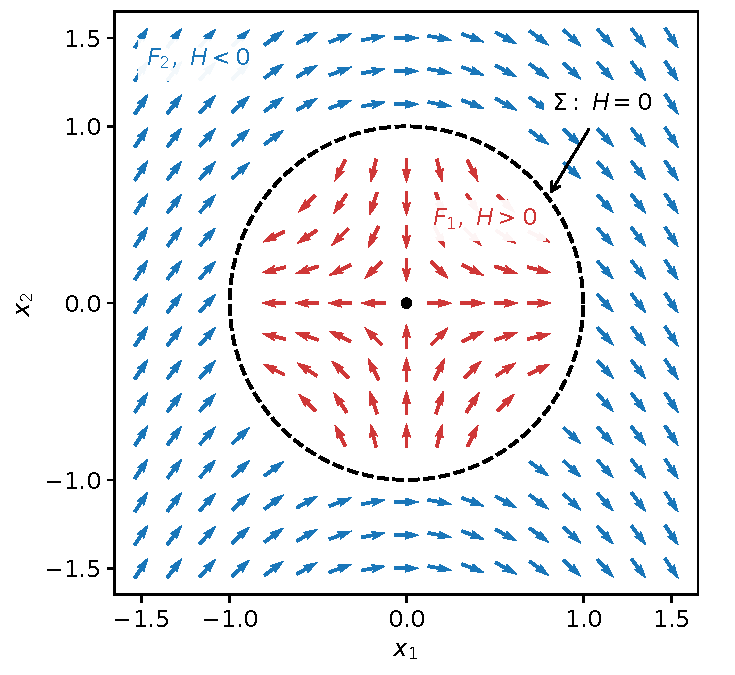
\includegraphics[width=.78\linewidth]{graphics_v3/circle_switch_fields.pdf}
\caption{Konkrét szakaszos vektormező a \eqref{eq:circle_switch_H}--\eqref{eq:circle_switch_fields} definíciókkal. Piros nyilak: $F_1$ a kör belsejében; kék nyilak: $F_2$ kívül. A fekete szaggatott kör $H=0$. A nyilak egységes hosszúságúak, csak az irányt jelölik; az origóban $F_1=0$.}
\label{fig:kapcsolofelulet}
\end{figure}

Továbbá bevezetjük
\begin{equation}
H_x=(\nabla H)^\mathsf{T}=\begin{pmatrix}
\frac{\partial H}{\partial x_1}&\frac{\partial H}{\partial x_2} &\dots
\end{pmatrix}
\end{equation}
\noindent deriváltat. A körpéldában $H_x=(-2x_1,-2x_2)$, amely az egységkörön sehol sem nulla, és befelé mutat, összhangban a belső tartományban pozitív $H$ választásával. A normális irányt $\nabla H$ adja, amely $H$ növekedése felé mutat. Feltesszük, hogy $H$ sima és $H_x\neq0$ a kapcsolófelületen; a jegyzetben $H_x$ sorvektor.

\emph{Attracting sliding region} néven jelöljük a $\Sigma$ kapcsolófelület azon részhalmazát, melyre $H_xF_1<0$ és $H_xF_2> 0$ skalárszorzat teljesül. Ezt a részhalmazt $\Sigma_s$-ként jelöljük, ahol $s$ index a $sliding$-ra utal. A sliding region területén a két dinamikai rendszerhez tartozó trajektóriák kapcsolófelületre merőleges komponensei egymás felé, azaz befelé mutatnak. Sliding region tartományra mutat példát a \ref{fig:csuszofelulet}.~ábra.

A \ref{fig:csuszofelulet}.~ábrán ugyanazokat a konkrét $H$, $F_1$ és $F_2$ függvényeket használjuk, mint a \ref{fig:kapcsolofelulet}.~ábrán. A normális komponensek:
\begin{equation}\label{eq:circle_normal_components}
\ell_1=H_xF_1=2(x_2^2-x_1^2),\qquad
\ell_2=H_xF_2=2x_1(x_2-1).
\end{equation}
Az egységkörön $\ell_1<0$ akkor teljesül, ha $|x_1|>|x_2|$, míg $\ell_2>0$ pontosan a bal félkörön. Ezért az attracting sliding region
\begin{equation}\label{eq:circle_sliding_arc}
\Sigma_s=\{(\cos\theta,\sin\theta):3\pi/4<\theta<5\pi/4\}.
\end{equation}
A két végpontban $\ell_1=0$, ezért ezek érintési pontok, és a szigorú egyenlőtlenségekkel definiált tartományhoz nem tartoznak hozzá. A zöld nyilak a lentebb levezetett $F_s$ sliding vektormező irányát mutatják. Például $x=(-1,0)$ esetén $\ell_1=-2$, $\ell_2=2$, így $\alpha=1/2$ és $F_s=(0,1/2)^{\mathsf T}$: a mozgás itt felfelé halad.

\begin{figure}[htbp]
\centering
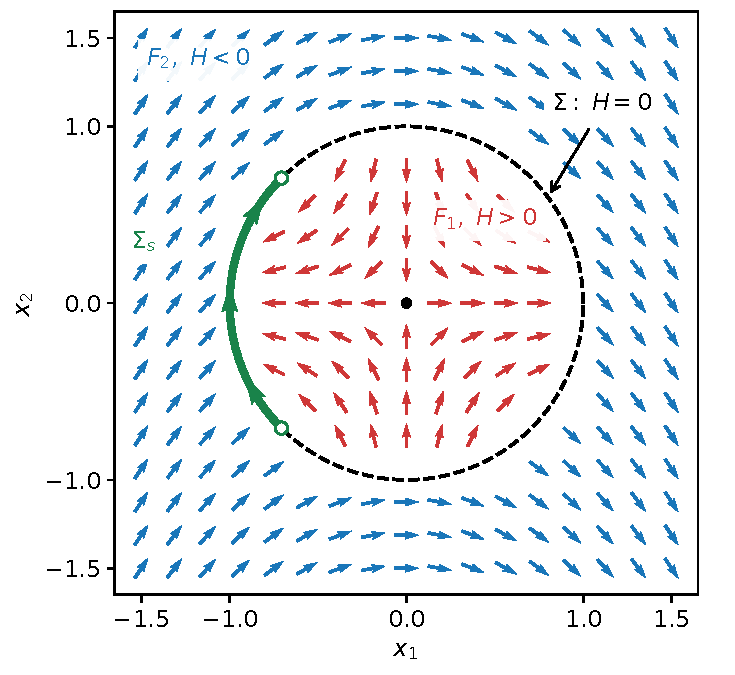
\includegraphics[width=.78\linewidth]{graphics_v3/circle_sliding_fields.pdf}
\caption{A \eqref{eq:circle_switch_H}--\eqref{eq:circle_switch_fields} mezőkhöz tartozó attracting sliding region (vastag zöld körív). A piros és kék nyilak $F_1$, illetve $F_2$, a zöld nyilak $F_s$ irányát mutatják; hosszuk nem sebességet jelöl. Az üres körök a tartomány végpontjai.}
\label{fig:csuszofelulet}
\end{figure}

A sliding region területén uralkodó dinamikát az
\begin{equation}
F_s=F_1(1-\alpha)+F_2\alpha
\end{equation}
\noindent egyenlet írja le. Vagyis lineárisan interpolálunk a két vektormező között oly módon, hogy $\alpha$-t úgy adjuk meg, hogy $H_xF_s=0$ teljesüljön. Ez akkor lesz igaz, ha $F_s$ és $H_x$ skaláris szorzata zérus:
\begin{equation}
H_xF_s =0 \,,
\end{equation}
\noindent tehát
\begin{equation}
H_xF_s = H_xF_1 (1-\alpha) + H_xF_2 \alpha = 0\,,
\end{equation}
\noindent melyből kifejezhető $\alpha$ értéke a következőképpen:
\begin{equation}
\alpha=\frac{H_xF_1}{H_x(F_1-F_2)}\,.
\end{equation}
A sliding dinamika a felület dimenziójára redukálódik, de általában nem szükségképpen egyszerű vagy stabil. Sliding mode control alkalmazásakor a kapcsolási törvényt és a felületet úgy tervezzük, hogy a felület elérhető legyen, és rajta a kívánt stabil dinamika alakuljon ki.

Jelölje $\ell_i=H_xF_i$ a normális komponenseket. Ha $\ell_1\ell_2>0$, transzverzális áthaladás történik. Az $\ell_1<0<\ell_2$ eset attracting sliding, míg $\ell_2<0<\ell_1$ repelling sliding: utóbbinál a felületre megszorított mező formálisan megadható, de az előrehaladó megoldás egyértelműsége külön vizsgálatot igényel. A $\ell_i=0$ határok érintési pontok. Attracting sliding esetén $0<\alpha<1$, így a kombináció konvex.

\section{Sliding mode control: munkahenger pozíciószabályozása}
\examplebody


Tekintsük a \ref{fig:munkahenger}.~ábrán látható elrendezést, mely munkahenger pozíciójának sliding mode control alapú szabályozására mutat példát. A hidraulikus tápegység (nyomásforrás) valamekkora $\Delta \tilde{p}>0$ konstans nyomást tud kiadni. A hengervezérlő szelep állásától függően a hidraulikus munkahengerbe $+\Delta \tilde{p}$ vagy $-\Delta \tilde{p}$ nyomás kerül. Ennek hatására a hengerfej jobbra vagy balra mozdul el. Célunk, hogy a munkahengert $x_{\rm k}$ kívánt pozícióba juttassuk a munkahenger sliding mode control alapú szabályozása által. Ehhez rendelkezésünkre áll egy PD szabályozó.

\begin{figure}[htbp]
\centering
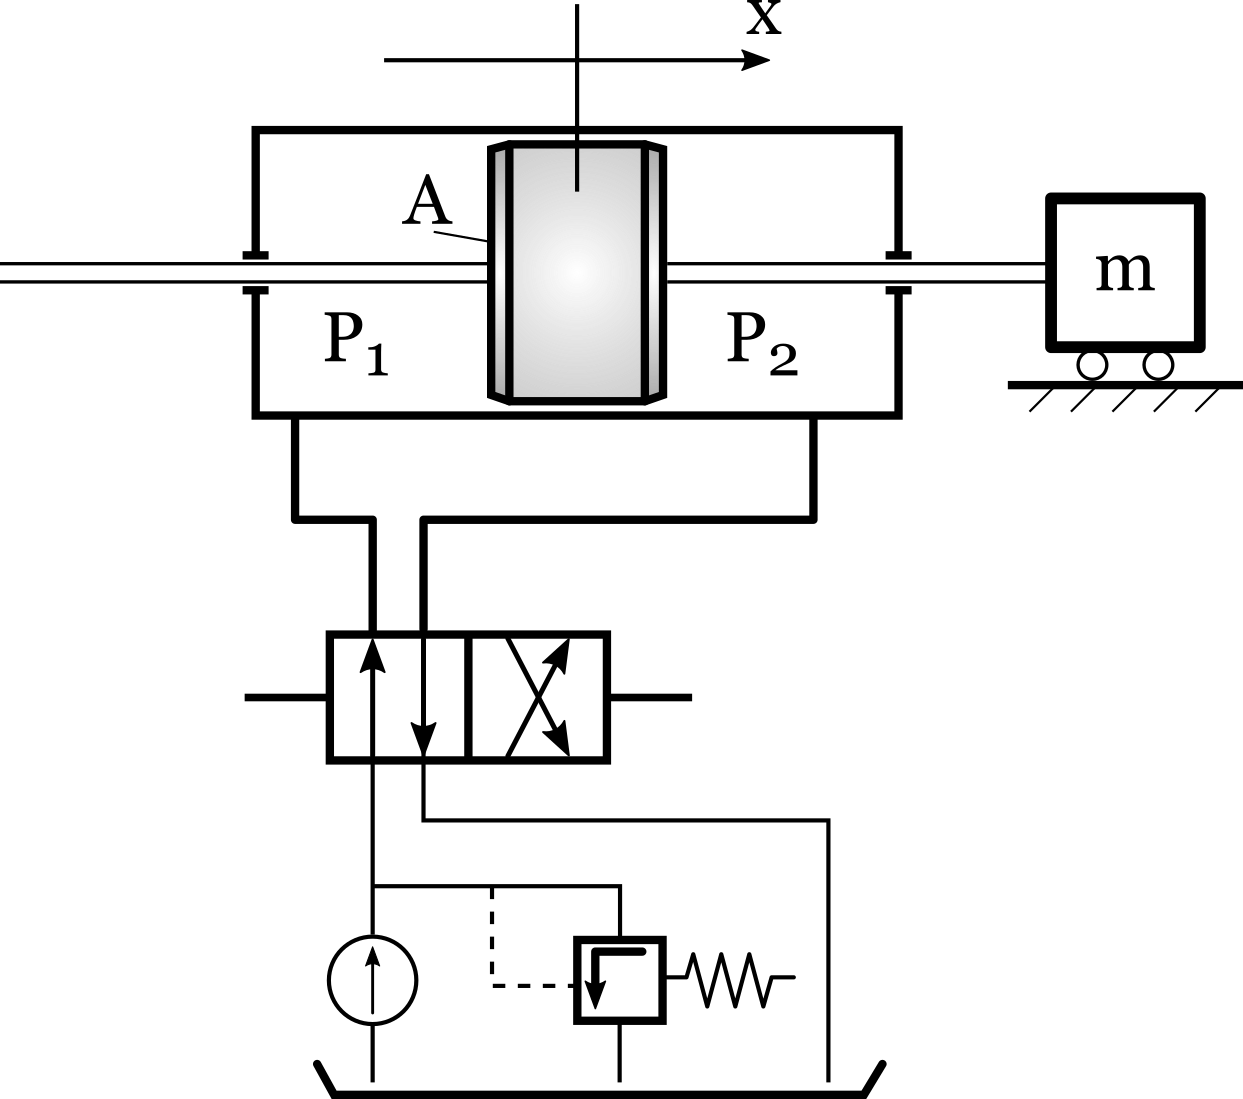
\includegraphics[width=0.5\textwidth]{graphics/munkahenger_fancy.png}
\caption{Munkahenger szabályozása.}
\label{fig:munkahenger}
\end{figure}

A dugattyú mozgását az alábbi másodrendű differenciálegyenlettel írhatjuk le:
\begin{equation}
m \ddot{x} + k \dot{x} = A \Delta p,
\end{equation}
\noindent ahol
\begin{equation}
	\Delta p = p_1- p_2 = \left\{
	\begin{matrix}
	+\Delta \tilde{p}, \mathrm{ha} & H(x) > 0\\
	-\Delta \tilde{p}, \mathrm{ha} & H(x) < 0
	\end{matrix}\,.
	\right.
\end{equation}
\indent A szabályozás során a munkahengert az $x_{\rm k} = 0$ pozícióba kívánjuk mozgatni. Ehhez a $H(x)$ függvényt egy PD szabályozási stratégia alapján írjuk elő:
\begin{equation} \label{eq:Hx}
H(x) = -P (x - x_{\rm k}) - D \dot{x} = -P x - D \dot{x},
\end{equation}
ahol az arányos és differenciáló tagok pozitívak: $P > 0$ és $D > 0$. A dinamikai rendszert az
\begin{equation}
x = (x_1 \; x_2)^{\rm T} = (x \; v)^{\rm T}
\end{equation}
\noindent változó bevezetésével elsőrendű alakra hozzuk. Ekkor a két vektormező a következő alakú:
\begin{equation}
F_1(x) = \left(
\begin{matrix}
x_2\\
\frac{A \Delta \tilde{p}}{m} - \frac{k}{m} x_2
\end{matrix}
\right), \quad
F_2(x) = \left(
\begin{matrix}
x_2\\
-\frac{A \Delta \tilde{p}}{m} - \frac{k}{m} x_2
\end{matrix}
\right).
\end{equation}
\noindent Mivel $\dot{x}=v=x_2$, a $H(x)$ által meghatározott kapcsolóvonal egyenlete a \eqref{eq:Hx}~egyenlet alapján
\begin{equation}
\Sigma = \left\{x: x_2 = -\frac{P}{D} x_1 \right\}\,,
\end{equation}
\noindent a kapcsolóvonalra merőleges irányt kijelölő $H_x$ gradiens pedig
\begin{equation}
H_x = \begin{pmatrix}-P&-D\end{pmatrix} \,.
\end{equation}

A kapcsolóvonal $\Sigma_{\rm s}$ sliding region része a
\begin{equation}
H_xF_1 = -P x_2 - \frac{D A \Delta \tilde{p}}{m} + \frac{D k}{m} x_2 < 0 \,,
\end{equation}
\noindent valamint az
\begin{equation}
H_xF_2 = -P x_2 + \frac{D A \Delta \tilde{p}}{m} + \frac{D k}{m} x_2 > 0
\end{equation}
\noindent egyenlőtlenségek által adott. Összevonva, még osztás nélkül:
\begin{equation}\label{eq:cylinder_sliding_condition}
-DA\Delta\tilde p<(Dk-Pm)x_2<DA\Delta\tilde p.
\end{equation}
Ha $Dk-Pm\neq0$, ebből a sliding region:
\begin{equation}
\Sigma_{\rm s} = \{x\in\Sigma: -x_2^* < x_2 < x_2^* \} \,,
\end{equation}
\noindent ahol
\begin{equation} \label{eq:x2csillag}
x_2^* = \frac{D A \Delta \tilde{p}}{|D k - P m|},\qquad Dk\neq Pm\,.
\end{equation}

A \eqref{eq:x2csillag} képlet ebben az esetben nem használható, mert nullával osztanánk. Ez azonban csak a tartomány végpontját megadó képlet korlátja: a vektormezők és a mozgásegyenletek továbbra is értelmesek. Visszatérve a \eqref{eq:cylinder_sliding_condition} osztás előtti feltételéhez, annak középső tagja minden véges $x_2$ esetén nulla. Mivel $D,A,\Delta\tilde p,m>0$, a két normális komponens
\begin{equation}\label{eq:cylinder_matched_normals}
H_xF_1=-\frac{DA\Delta\tilde p}{m}<0,\qquad
H_xF_2=+\frac{DA\Delta\tilde p}{m}>0.
\end{equation}
Tehát mindkét oldalról a kapcsolóvonal felé mutat a mező, annak minden pontjában:
\begin{equation}
\Sigma_s=\Sigma \qquad (Dk=Pm).
\end{equation}
Nincsenek véges végpontok. Az $x_2^*\to\infty$ határérték ezt a korlátlan kiterjedést fejezi ki, nem végtelen sebességet vagy szinguláris mozgást.

A kapcsolóvonal elérése is különösen egyszerűvé válik: a $\dot H=H_x\dot x$ azonosság és \eqref{eq:cylinder_matched_normals} alapján
\begin{equation}
\dot H=-\frac{DA\Delta\tilde p}{m}\operatorname{sgn}(H),\quad H\neq0,
\qquad
 t_{\rm el}=\frac{m|H(x(0))|}{DA\Delta\tilde p}.
\end{equation}
Az ideális modellben tehát minden véges kezdeti állapotból véges idő alatt elérjük a kapcsolóvonalat. Utána a Filippov-féle sliding megoldást kell használni, amely $H=0$-n tartja a pályát; itt nem a két klasszikus mező valamelyikét választjuk tartósan.

A két vektormezőt, a kapcsolófelületet és a sliding region tartományt szemlélteti a \ref{fig:csuszomod_szabalyozas}.~ábra.

\begin{figure}[ht]
\centering
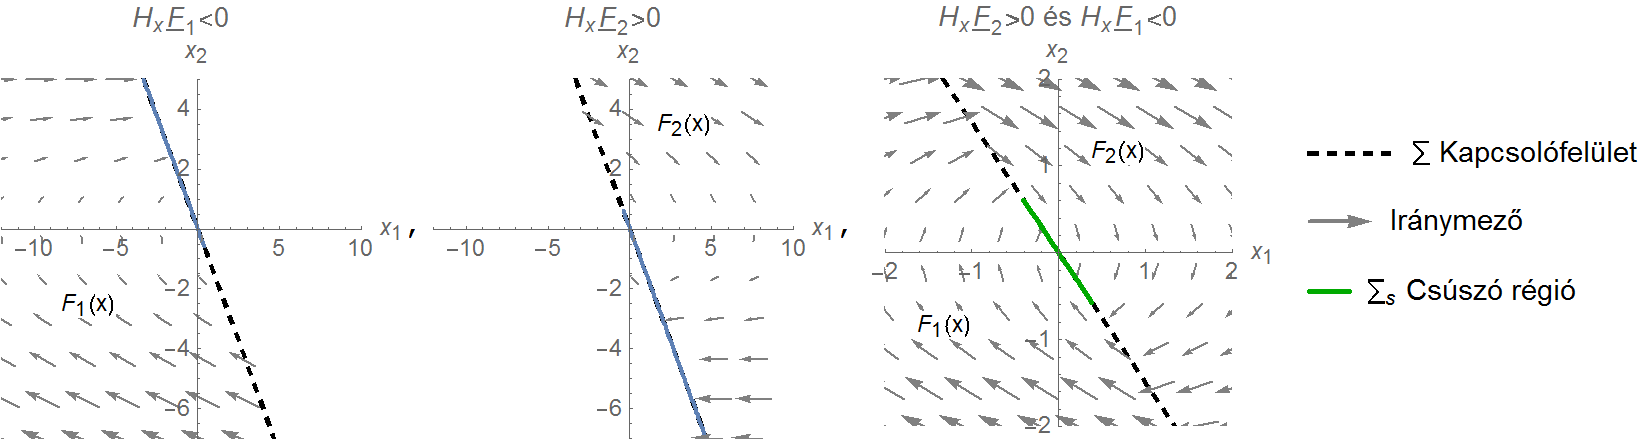
\includegraphics[width=\textwidth,trim={0.000bp 0.000bp 4.499bp 0.750bp},clip]{graphics/sliding_region_PELDA.png}
\caption{Munkahenger sliding mode control alapú szabályozása.}
\label{fig:csuszomod_szabalyozas}
\end{figure}

A $\Sigma_{\rm s}$-en érvényes dinamikát a korábban leírt
\begin{equation}
F_s = F_1 (1-\alpha) + F_2 \alpha
\end{equation}
\noindent vektormező határozza meg, ahol
\begin{equation}
\alpha = \frac{H_xF_1}{H_x(F_1-F_2)} = \frac{-P x_2 -D \left(\frac{A \Delta \tilde{p}}{m} - \frac{k}{m} x_2\right)}{-D \frac{2A \Delta \tilde{p}}{m}} \,.
\end{equation}
A nevező $H_x(F_1-F_2)=-2DA\Delta\tilde p/m$ nem nulla akkor sem, ha $Dk-Pm=0$: a Filippov-kombináció tehát ilyenkor is jól definiált. A keverési tényező egyszerűbb alakja
\begin{equation}
\alpha=\frac12-\frac{(Dk-Pm)x_2}{2DA\Delta\tilde p}.
\end{equation}
A különleges esetben $\alpha=1/2$ a teljes kapcsolóvonalon, vagyis $F_s=(F_1+F_2)/2$. A két ellentétes nyomáserő a konvex kombinációban kiegyenlíti egymást, és $\dot x_2=-(k/m)x_2$ marad. A $Dk=Pm$, azaz $P/D=k/m$ illesztés miatt éppen ez a csillapított mozgás tartja a pályát a kapcsolóvonalon.

Ezt $F_s$-be visszahelyettesítve, a kapcsolóvonalra megszorított dinamika
\begin{equation}
\begin{split}
F_s & = F_1 (1-\alpha) + F_2 \alpha = F_1 + \alpha (F_2-F_1) =  \\ & =
\begin{pmatrix}
x_2\\
\frac{A \Delta \tilde{p}}{m} - \frac{k}{m} x_2
\end{pmatrix} +
\alpha \begin{pmatrix}
0 \\
-\frac{2A \Delta \tilde{p}}{m}
\end{pmatrix} =
\begin{pmatrix}
x_2 \\
-\frac{P}{D}x_2
\end{pmatrix}
\end{split}
\end{equation}
\noindent vagyis
\begin{equation}
\left. \dot{x}_1 \right|_{\Sigma_s} = x_2, \qquad \left. \dot{x}_2 \right|_{\Sigma_s} = -\frac{P}{D} x_2.
\end{equation}

\underline{Megjegyzés:} $F_s$ második komponensét a $\Sigma$ kapcsolóvonal egyenletének idő szerinti deriválásával is meg lehet kapni.

A kapcsolóvonalon $x_2=-(P/D)x_1$, ezért a sliding megoldás exponenciálisan tart az origóhoz, $P/D$ lecsengési rátával. A sliding feltétele közvetlenül a két normális komponens előjeléből:
\[
|(Dk-Pm)x_2|<DA\Delta\tilde p.
\]
Pozitív fizikai paramétereknél és $Dk\neq Pm$ esetén tehát mindkét előjelű $Dk-Pm$ mellett létezik nemüres sliding region. A $Pm<Dk$ feltétel nem szükséges. Ha $Dk=Pm$, a teljes kapcsolóvonal attracting sliding region, de az origó elérése ettől nem válik pillanatszerűvé. A $t_{\rm el}$ elérési időtől kezdve
\begin{equation}
x_1(t)=x_1(t_{\rm el})e^{-(k/m)(t-t_{\rm el})},\qquad
x_2(t)=-\frac{k}{m}x_1(t).
\end{equation}
A kapcsolóvonalat tehát véges idő alatt érjük el, az origóhoz pedig általában csak aszimptotikusan tartunk; a lecsengés időállandója $m/k=D/P$.

A $P/D$ arány növelése gyorsítja a sliding dinamika lecsengését, de a tartomány mérete $1/|k-mP/D|$ szerint változik: először növekedhet, majd a $P/D=k/m$ érték fölött csökken. Véges pozitív paramétereknél nem tűnik el. A \ref{table:parameter}. táblázat értékeivel $Pm=0{,}21$, $Dk=0{,}02$, és $x_2^*\approx0{,}5263\,\mathrm{m/s}$, ami összhangban van a sliding lehetőségével.

Szimulációs példát mutat a \ref{fig:sliding_mode_control}.~ábra. A szimuláció során felhasznált paraméterértékeket a \ref{table:parameter}.~táblázat tartalmazza. $x_1(0) = -12$~m és $x_2(0) = 0.2$~m/s kezdeti feltételekkel indítva a szimulációt, a kapcsolófelületen áthaladva, a sliding region tartományba kerül a megoldás, majd a rendszer a kapcsolóvonalon tart a $(0 \; 0)^{\rm T}$ egyensúlyi helyzethez.
\begin{table}[htbp]
	\caption{Paraméterértékek}
	\vspace{0.1 cm}
	\centering
	\begin{tabular}{|c|c|c|c|c|c|} \hline
	$P$ [1/s] & $D$ [1] & $m$ [kg] & $A$ $[{\rm m}^2]$ & $\Delta \tilde{p}$ [Pa] & $k$ [Ns/m] \\ 	\hline
	$0.3$ & $0.2$ & $0.7$ & $0.5$ & $1$ & $0.1$ \\ \hline
	\end{tabular}
	\label{table:parameter}
\end{table}
\begin{figure}[ht]
\centering
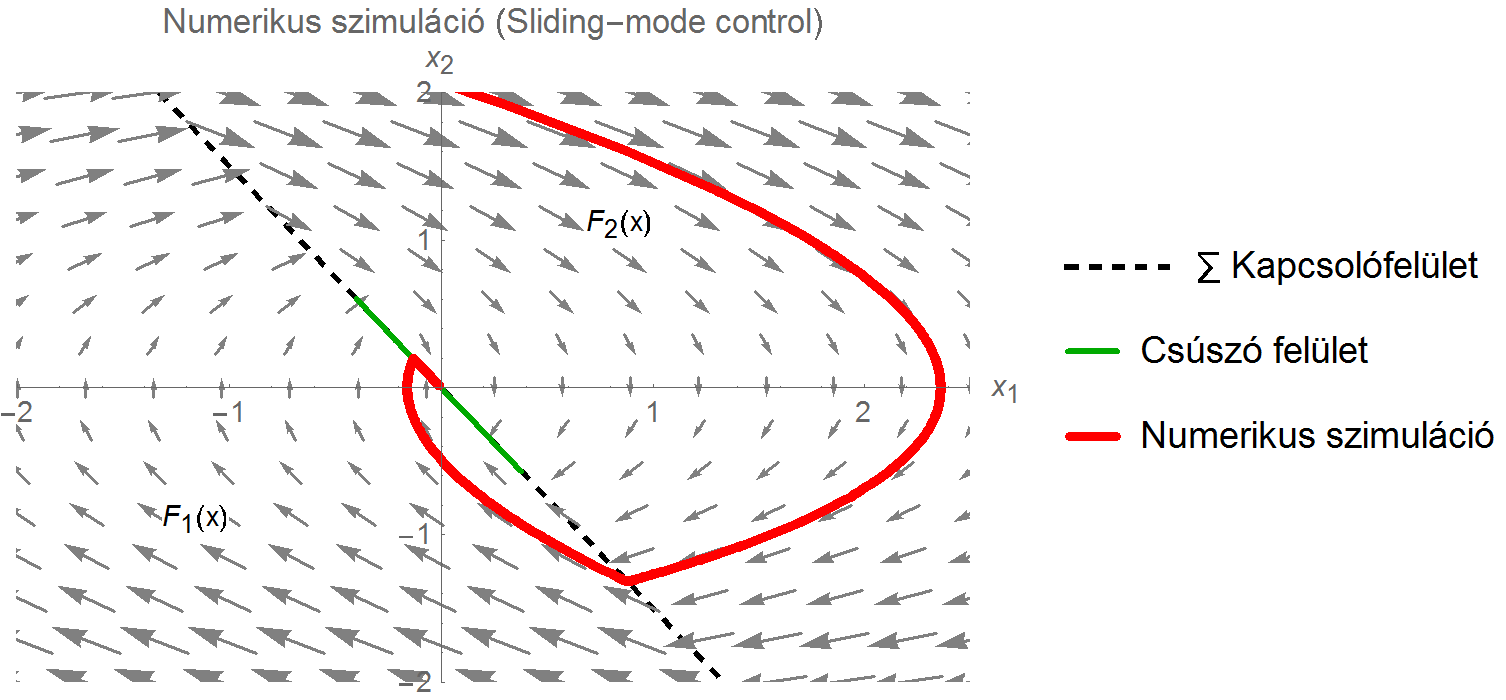
\includegraphics[width=\textwidth,trim={0.000bp 2.250bp 5.249bp 2.250bp},clip]{graphics/sliding_mode_control.png}
\caption{A sliding mode control által eredményezett trajektória. Kezdeti feltételek: $x_1(0) = -12$~m, $x_2(0) = 0.2$~m/s.}
\label{fig:sliding_mode_control}
\end{figure}
\exampleend


\chapter{\label{sec:korr_kapcs}Korrekció a kapcsolófelületen}

\section{Transzverzális metszés, hibrid dinamikai rendszer}
A közös időpontra korrigáló leképezés könyvbeli levezetése: \cite[2.5.1--2.5.2. szakasz]{dib}. A következő számítás az ottani transzverzális eseménygeometriát részletezi.

A korrekciós mátrix levezetéséhez lásd \cite{kong}.
Legyen $\dot{x}=F(x)$ a folytonos dinamika, $\Sigma=\{x:H(x)=0\}$ az eseményfelület, $x^+=R(x^-)$ a reset leképezés. A megoldásoperátor $\Phi(x,t)$. Feltesszük, hogy $F,H,R$ simák és $H_x(x^*)F(x^*)\neq0$ a vizsgált ütközési pontban.

A referenciapálya a $t_1$ időpontban éri el az $x^*$ eseménypontot, majd az állapota $R(x^*)$-ra ugrik. A közeli kezdeti állapotból indított, perturbált pálya általában más időpontban éri el a felületet: legyen ez $t_1+\delta$. A $\delta$ tehát \emph{eseményidő-eltérés}, amely a perturbációtól függ, és pozitív vagy negatív is lehet. Pozitív értéke későbbi, negatív értéke korábbi ütközést jelent.

A stabilitásvizsgálathoz a két pálya eltérését \emph{azonos időpontban} kell összehasonlítanunk. Az $R_x$ önmagában csak az eseményfelületen vett reset leképezés érzékenységét adná meg; nem venné figyelembe, hogy a megzavart pálya más ideig mozog az esemény előtt és után. Ezért bevezetünk egy olyan $Q$ leképezést, amely a perturbált pálya esemény előtti leírását a referencia $t_1$ idejére vonatkozó esemény utáni leírásba viszi át.

Legyen $x_0=x^*+\Delta x$ az esemény előtti sima dinamika szerint $t_1$-ig továbbvezetett perturbált állapot. Ez \emph{segédállapot}: ha a perturbált ütközés korábban történt ($\delta<0$), akkor a tényleges pálya $t_1$-ben már az esemény utáni dinamikát követi, és nem $x_0$-ban van. A sima folytatás éppen azért szükséges, hogy ugyanazon referenciaidőben adhassuk meg a bemenő perturbációt.

A keresett korrekciós leképezés a \ref{fig:korr_idokorrekcio}. ábra jelöléseivel:
\begin{equation}\label{eq:Q_osszetetel}
Q(x_0)=\Phi\bigl(R(\Phi(x_0,\delta)),-\delta\bigr).
\end{equation}
\begin{figure}[htbp]\centering
% Native vector figure. Font sizes are fixed in the final document, no scaling.
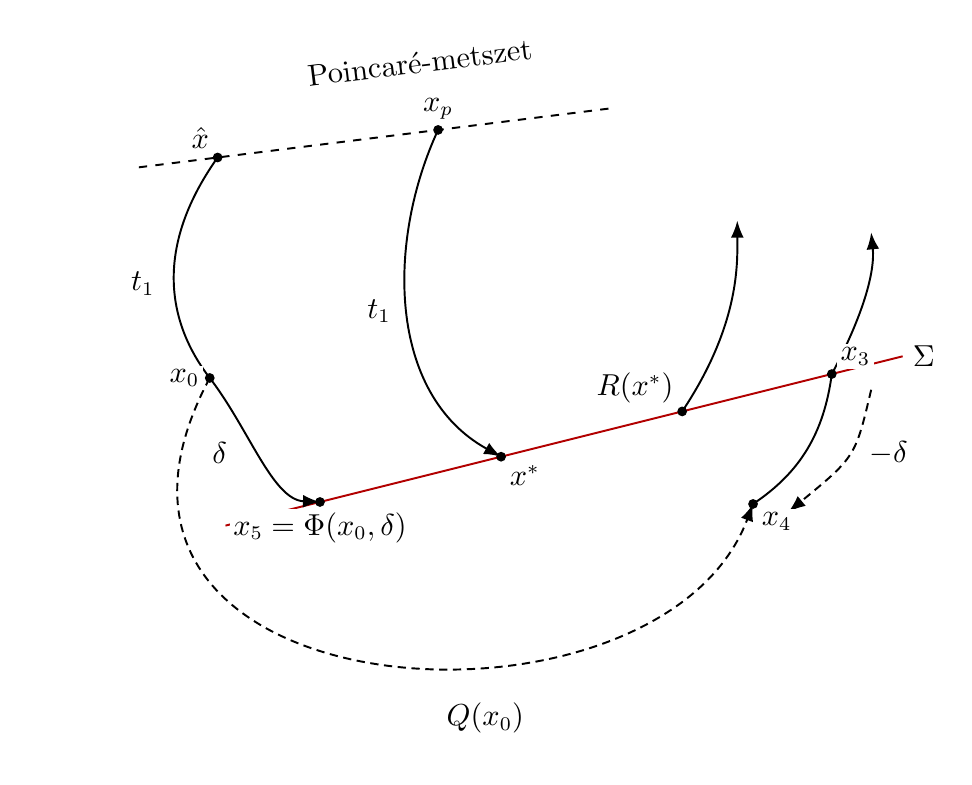
\begin{tikzpicture}[x=1cm,y=1cm,>=Latex,line width=.7pt,
 font=\normalfont\fontsize{10.5}{12.6}\selectfont,
 every label/.style={fill=white,inner sep=1.3pt},
 point/.style={circle,fill,inner sep=1.25pt}]
\coordinate (xp) at (5.2,5.95);
\coordinate (xh) at (2.4,5.6);
\coordinate (x0) at (2.3,2.8);
\coordinate (xs) at (6,1.8);
\coordinate (x5) at (3.7,1.225);
\coordinate (rs) at (8.3,2.375);
\coordinate (x3) at (10.2,2.85);
\coordinate (x4) at (9.2,1.2);
\draw[dashed] (1.4,5.475)--(7.4,6.225);
\node[above,rotate=7] at (5,6.55) {Poincaré-metszet};
\draw[red!70!black] (2.5,.925)--(11.1,3.075)
 node[right,black] {$\Sigma$};
\draw[->] (xp)..controls(4.55,4.55)and(4.55,2.6)..(xs);
\draw (xh)..controls(1.55,4.4)and(1.8,3.45)..(x0);
% Matching Bezier derivatives at x0: (2.3,2.8)-(1.8,3.45)=(2.8,2.15)-(2.3,2.8).
\draw[->] (x0)..controls(2.8,2.15)and(3.1,1.25)..(x5);
\draw[->] (rs)..controls(9.05,3.5)and(9,4.3)..(9,4.8);
\draw (x4)..controls(9.8,1.6)and(10.1,2.1)..(x3);
\draw[->] (x3)..controls(10.6,3.6)and(10.75,4.15)..(10.7,4.65);
\draw[densely dashed,->] (x0)..controls(0,-1.5)and(8,-2)..(x4);
\node[below] at (5.8,-1.2) {$Q(x_0)$};
\draw[densely dashed,->] (10.7,2.65)..controls(10.5,1.8)..(9.65,1.1);
\node[right] at (10.55,1.85) {$-\delta$};
\node at (1.45,4.0) {$t_1$};
\node at (4.45,3.65) {$t_1$};
\node[left] at (2.65,1.85) {$\delta$};
\node[point,label=above:$x_p$] at (xp) {};
\node[point,label=above left:$\hat x$] at (xh) {};
\node[point,label=left:$x_0$] at (x0) {};
\node[point,label=below right:$x^*$] at (xs) {};
\node[point,label=below:{$x_5=\Phi(x_0,\delta)$}] at (x5) {};
\node[point,label=above left:{$R(x^*)$}] at (rs) {};
\node[point,label=above right:$x_3$] at (x3) {};
\node[point,label=below right:$x_4$] at (x4) {};
\end{tikzpicture}

\caption{A referencia- és a perturbált esemény időbeli összehangolása.}
\label{fig:korr_idokorrekcio}
\end{figure}

Az \eqref{eq:Q_osszetetel} összetételt belülről kifelé, három lépésben értelmezzük:
\begin{enumerate}
\item \textbf{Eljutunk a perturbált eseményhez.} Az $x_0$ segédállapotból $\delta$ időt lépünk a sima megoldásoperátorral. Az így kapott $x_5=\Phi(x_0,\delta)$ már a kapcsolófelületen van: ez a perturbált pálya tényleges, esemény előtti állapota a $t_1+\delta$ időpontban.
\item \textbf{Alkalmazzuk a reset leképezést.} Az $x_3=R(x_5)$ pont az esemény utáni állapot, ugyanabban a $t_1+\delta$ időpontban. Ütközésnél például ebben a lépésben fordul meg és csökken a normális sebesség.
\item \textbf{Visszatérünk a közös referenciaidőre.} Az esemény utáni $x_3$ állapotot $-\delta$ idővel továbbvezetjük: $x_4=\Phi(x_3,-\delta)=Q(x_0)$. Ezzel ismét a $t_1$ időpontra vonatkozó állapotot kapunk, amelyet már $R(x^*)$-gal kell összehasonlítani.
\end{enumerate}
A harmadik lépésben szereplő negatív idő \emph{matematikai időkorrekció}, nem fizikailag visszafelé lejátszott ütközés. Ha $\delta>0$, az esemény utáni sima pályát visszafelé hosszabbítjuk meg; ha $\delta<0$, előrefelé vezetjük a referenciaidőig. Az itt vizsgált speciális esetben az esemény előtt és után ugyanaz az $F$ mező érvényes, ezért mindkét helyen ugyanazt a $\Phi$ operátort használjuk. Különböző mezők esetén a belső operátor $\Phi_1$, a külső $\Phi_2$, ahogy a \ref{sec:altalanos_korrekcio}. szakaszban látni fogjuk.

A $\delta$ nem független bemenő adat: a közeli eseménypontot a
\[
H\bigl(\Phi(x_0,\delta(x_0))\bigr)=0,\qquad \delta(x^*)=0
\]
feltétel jelöli ki. Mivel ennek $\delta$ szerinti deriváltja a referenciapontban $H_x(x^*)F(x^*)\neq0$, az implicitfüggvény-tétel lokálisan egyértelmű, sima $\delta(x_0)$ függvényt biztosít. Következésképpen $Q$ a választott esemény közelében jól definiált sima leképezés. Nem azt feltételezzük, hogy a teljes hibrid pálya visszafordítható, hanem csak a sima szakaszok lokális folytatását használjuk.

Perturbáció nélkül $x_0=x^*$ és $\delta=0$, így \eqref{eq:Q_osszetetel} szerint $Q(x^*)=R(x^*)$. Kis perturbációnál a releváns esemény utáni eltérés ezért $Q(x^*+\Delta x)-R(x^*)$. Ennek elsőrendű tagját adja majd a $Q_x(x^*)\Delta x$ szorzat; az eseményidő változásának hatása jelenik meg a korrekciós mátrix $R_x$-en felüli tagjában.

Az eseményig történő elmozdulás első rendben:
\begin{align}
x_5&=x^*+\Delta x+\delta F(x^*)+\mathcal O(2),\\
0=H(x_5)&=H_x(x^*)\Delta x+\delta H_x(x^*)F(x^*)+\mathcal O(2),\\
\delta&=-\frac{H_x(x^*)\Delta x}{H_x(x^*)F(x^*)}+\mathcal O(2).
\end{align}
Az $\mathcal O(2)$ jelölés a perturbáció és az eseményidő-eltérés legalább másodrendű tagjait foglalja össze. A reset leképezést és az időkorrekciót is sorba fejtve:
\begin{align}
Q(x_0)&=R(x^*)+R_x(x^*)\Delta x\notag\\
&\quad+\delta\bigl[R_x(x^*)F(x^*)-F(R(x^*))\bigr]+\mathcal O(2).
\label{linearizaltx4}
\end{align}
Ezért
\begin{equation}\label{linearizaltlekepezes}
Q(x_0)=R(x^*)+Q_x(x^*)\Delta x+\mathcal O(\|\Delta x\|^2),
\end{equation}
ahol a korrekciós, más néven saltation-mátrix
\begin{equation}\label{eq:Qxmatrix}
Q_x=R_x+\frac{\bigl[F(R(x^*))-R_xF(x^*)\bigr]H_x}{H_xF(x^*)}.
\end{equation}
Itt $H_x$ egy $1\times n$ sorvektor; a számlálóban oszlop- és sorvektor diadikus szorzata áll, tehát $Q_x\in\mathbb R^{n\times n}$.

\section{Példa: gerjesztett ütköző oszcillátor}
\examplebody

A \eqref{eq:Qxmatrix} képletet most háromdimenziós állapottérben, tényezőnként számítjuk ki. Használjuk az $x=(u,v,s)^{\mathsf T}$ állapotot: $u$ az elmozdulás, $v$ a sebesség, $s$ pedig az időt követő állapotváltozó ($\dot s=1$). A csillapítás $\zeta$, a visszapattanási tényező $r$:
\[
F(x)=\begin{pmatrix}v\\-u-2\zeta v+\cos(\omega s)\\1\end{pmatrix},\qquad
H(x)=u-\sigma,\qquad R(x)=\begin{pmatrix}u\\-rv\\s\end{pmatrix}.
\]
A fal helyzete $\sigma$; ezt megkülönböztetjük a $\delta$ időkorrekciótól. Az ütközés előtti eseménypont legyen $x^*=(\sigma,v^-,s^*)^{\mathsf T}$, az utána következő állapot pedig $R(x^*)=(\sigma,-rv^-,s^*)^{\mathsf T}$. A felső $-$ és $+$ jel az esemény előtti és utáni értéket jelöli, nem hatványt.


A reset leképezés és az eseményfüggvény deriváltját elemenként felírva:
\[
R_x=\begin{pmatrix}1&0&0\\0&-r&0\\0&0&1\end{pmatrix},\qquad
H_x=\begin{pmatrix}1&0&0\end{pmatrix}.
\]
A \eqref{eq:Qxmatrix} képlet minden tagját az eseménypontban értékeljük ki; röviden $F^-=F(x^*)$, $F^+=F(R(x^*))$. Először ezeket a vektorokat számítjuk ki, majd közvetlenül behelyettesítjük a korrekciós képletbe.


Az ütközéskor a sebesség előjelet és nagyságot vált, míg $u$ és $s$ nem ugrik. Emiatt
\[
a^-=-\sigma-2\zeta v^-+\cos(\omega s^*),\qquad
 a^+=-\sigma+2\zeta r v^-+\cos(\omega s^*),
\]
\[
F^-=\begin{pmatrix}v^-\\a^-\\1\end{pmatrix},\qquad
F^+=\begin{pmatrix}-rv^-\\a^+\\1\end{pmatrix}.
\]
Bár ugyanaz az $F$ függvény írja le a szabad mozgást az ütközés előtt és után, különböző állapotokban értékeljük ki, ezért általában $F^+\neq F^-$.

A konkrét tényezőkkel a teljes behelyettesítés:
\[
Q_x=
\begin{pmatrix}1&0&0\\0&-r&0\\0&0&1\end{pmatrix}
+\frac{
\left[
\begin{pmatrix}-rv^-\\a^+\\1\end{pmatrix}
-\begin{pmatrix}1&0&0\\0&-r&0\\0&0&1\end{pmatrix}
\begin{pmatrix}v^-\\a^-\\1\end{pmatrix}
\right]\begin{pmatrix}1&0&0\end{pmatrix}}
{\begin{pmatrix}1&0&0\end{pmatrix}\begin{pmatrix}v^-\\a^-\\1\end{pmatrix}}.
\]
A nevező egy skalár; a számlálóban az oszlopvektor és a sorvektor külső szorzata áll. A következő lépésekben ezeket külön kiszámítjuk.


Először a reset leképezés deriváltját szorozzuk az ütközés előtti vektormezővel:
\[
R_xF^-=\begin{pmatrix}1&0&0\\0&-r&0\\0&0&1\end{pmatrix}
\begin{pmatrix}v^-\\a^-\\1\end{pmatrix}
=\begin{pmatrix}v^-\\-ra^-\\1\end{pmatrix}.
\]
Ezt vonjuk ki az esemény utáni mezőből:
\[
b:=F^+-R_xF^-=\begin{pmatrix}-(1+r)v^-\\a^++ra^-\\0\end{pmatrix}.
\]
A nevező pedig
\[
H_xF^-=\begin{pmatrix}1&0&0\end{pmatrix}
\begin{pmatrix}v^-\\a^-\\1\end{pmatrix}=v^-.
\]
Ez az eseményfelület normális irányú sebessége. A transzverzalitási feltétel itt pontosan $v^-\neq0$.


Az oszlopvektort jobbról szorozzuk a sorvektorral:
\[
bH_x=
\begin{pmatrix}-(1+r)v^-\\a^++ra^-\\0\end{pmatrix}
\begin{pmatrix}1&0&0\end{pmatrix}
=\begin{pmatrix}
-(1+r)v^-&0&0\\a^++ra^-&0&0\\0&0&0
\end{pmatrix}.
\]
Általában $(bH_x)_{ij}=b_i(H_x)_j$. Itt csak az első oszlop nem nulla, mert $H_x=(1,0,0)$: az eseményidő elsőrendű változását közvetlenül az elmozdulás perturbációja határozza meg.
A skalár nevezővel való osztás, majd $R_x$ hozzáadása:
\[
\begin{aligned}
Q_x&=\begin{pmatrix}1&0&0\\0&-r&0\\0&0&1\end{pmatrix}
+\begin{pmatrix}-(1+r)&0&0\\(a^++ra^-)/v^-&0&0\\0&0&0\end{pmatrix}\\[2mm]
&=\begin{pmatrix}-r&0&0\\(a^++ra^-)/v^-&-r&0\\0&0&1\end{pmatrix},\qquad v^-\neq0.
\end{aligned}
\]
A gyorsulásokat behelyettesítve a középső sor első eleme tovább egyszerűsíthető, mert a csillapítási tagok kiesnek:
\[
a^++ra^-=(1+r)\bigl[-\sigma+\cos(\omega s^*)\bigr].
\]


A $Q_x$ az azonos referenciaidőben értelmezett perturbációkat kapcsolja össze. Ha $\Delta x=(\Delta u,\Delta v,\Delta s)^{\mathsf T}$, akkor első rendben
\[
\Delta Q=
\begin{pmatrix}-r&0&0\\(a^++ra^-)/v^-&-r&0\\0&0&1\end{pmatrix}
\begin{pmatrix}\Delta u\\\Delta v\\\Delta s\end{pmatrix}
=\begin{pmatrix}
-r\,\Delta u\\
\dfrac{a^++ra^-}{v^-}\Delta u-r\,\Delta v\\
\Delta s
\end{pmatrix}.
\]
Ez magyarázza, hogy az első diagonális elem $-r$, miközben $R_x$ első diagonális eleme $1$: a $Q_x$ a reset leképezés mellett az eltérő eseményidő korrekcióját is tartalmazza. Az $(a^++ra^-)/v^-$ elem azt írja le, hogyan okoz az elmozdulás perturbációja a módosult ütközési időn keresztül sebességeltérést.

A $v^-\to0$ határesetben a transzverzális levezetés érvényét veszti; ezt a grazing-fejezet tárgyalja. Még ha a számláló is nullává válik, a fenti képlet önmagában nem igazol érvényes korrekciós mátrixot az érintési pontban.
\exampleend

\section{Transzverzális metszés, általános eset}\label{sec:altalanos_korrekcio}

Korrekció a kapcsolósíkon. Az általános esetben:
\[
{\dot{x}} = \begin{cases}
   {\ F}_1(x), & \text{ha } \; H({ x})>0 \\
   {\ F}_2(x), & \text{ha } \; H({ x})<0,
 \end{cases}
\]

\begin{figure}
	\centering
	% All labels have the same final 10.5 pt font as the other chapter-3 drawings.
\begin{tikzpicture}[x=1cm,y=1cm,>=Latex,line width=.7pt,
 font=\normalfont\fontsize{10.5}{12.6}\selectfont,
 every label/.style={fill=white,inner sep=1.3pt},
 point/.style={circle,fill,inner sep=1.25pt}]
\coordinate (xm) at (4,1.3);
\coordinate (xp) at (8.4,2.1);
\draw (2.5,.1)--(7,3.7) node[above] {$\Sigma=\{H=0\}$};
\draw[->] (2,4.5)..controls(1.4,2.7)and(2.4,1.9)..(xm);
\node[left] at (1.25,3.2) {$F_1$};
\draw[dashed,->] (xm)..controls(5.3,.1)and(7,.2)..(xp);
\node[below] at (6.1,.55) {$R$};
\draw[->] (xp)..controls(9.1,2.6)and(9.2,3.8)..(9.0,4.5);
\node[right] at (9.6,3.3) {$F_2$};
\node[point,label=below left:$x^-$] at (xm) {};
\node[point,label=below right:{$x^+=R(x^-)$}] at (xp) {};
\end{tikzpicture}

	\caption{$R(x)$ nem kapcsolósíkra képez le.}\label{fig:501}
\end{figure}

ahol ${x}\rightarrow R({x}),\; \text{ha}\; H(x)=0.$ Továbbá $R(x)$-nek nem kötelező a kapcsolósíkra leképeznie (lásd \ref{fig:501}. ábra).\\

 A $Q(x)$ korrekciós leképezés alatt a következő érthető: (lásd \ref{fig:502}. ábra)
\noindent
 $\Sigma = \lbrace x,\; H(x)=0 \rbrace,\\
 x^*=\Phi_1(x_p,t),\\
 x_0=\Phi_1{(\hat{x},t_1)} \rightarrow x_2=\Phi_1(x_0,\delta),\\
 x_4=\Phi_2(x_3,-\delta),\\
 x_0 \rightarrow x_4=Q(x_0)=\Phi_2(\underbrace{R(\overbrace{\Phi_1(x_0,\delta)}^{x_2})}_{x_3},-\delta)$

\begin{figure}[ht]
\centering
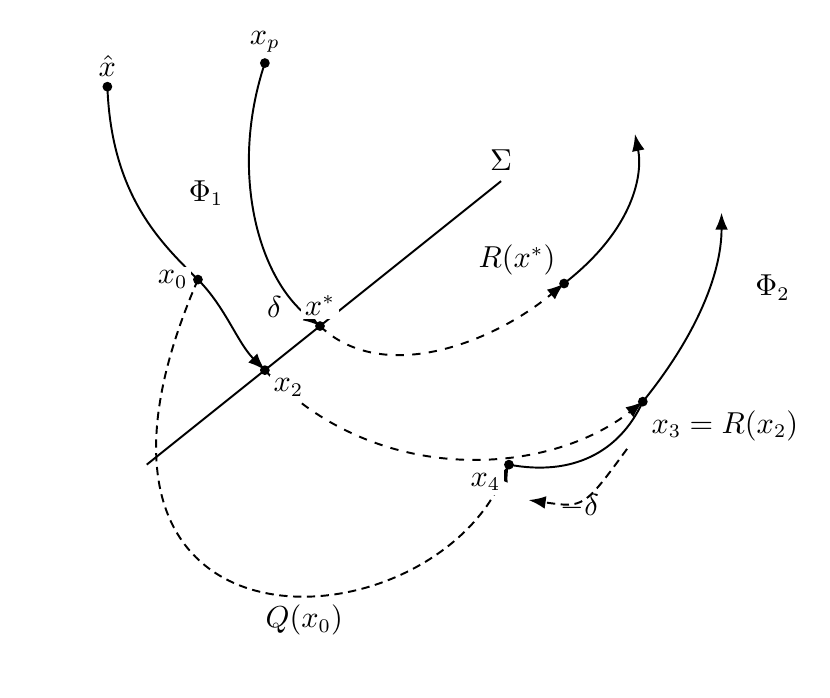
\begin{tikzpicture}[x=1cm,y=1cm,>=Latex,line width=.7pt,
 font=\normalfont\fontsize{10.5}{12.6}\selectfont,
 every label/.style={fill=white,inner sep=1.3pt},
 point/.style={circle,fill,inner sep=1.25pt}]
\coordinate (xp) at (4,5.9);
\coordinate (xh) at (2,5.6);
\coordinate (x0) at (3.15,3.15);
\coordinate (xs) at (4.7,2.56);
\coordinate (x2) at (4,2);
\coordinate (rs) at (7.8,3.1);
\coordinate (x3) at (8.8,1.6);
\coordinate (x4) at (7.1,.8);
\draw (2.5,.8)--(7,4.4) node[above] {$\Sigma$};
\draw[->] (xp)..controls(3.55,4.55)and(3.9,3.2)..(xs);
\draw (xh)..controls(2.05,4.2)and(2.7,3.6)..(x0);
\draw[->] (x0)..controls(3.5,2.8)and(3.65,2.35)..(x2);
\node[left] at (3.6,4.25) {$\Phi_1$};
\node[right] at (3.9,2.8) {$\delta$};
\draw[dashed,->] (xs)..controls(5.5,1.8)and(6.9,2.35)..(rs);
\draw[dashed,->] (x2)..controls(5.4,.5)and(7.6,.65)..(x3);
\draw[->] (rs)..controls(8.7,3.8)and(8.8,4.5)..(8.7,5.0);
\draw (x4)..controls(7.9,.65)and(8.5,.95)..(x3);
\draw[->] (x3)..controls(9.45,2.4)and(9.8,3.2)..(9.8,4.0);
\node[right] at (10.1,3.05) {$\Phi_2$};
\draw[densely dashed,->] (x0)..controls(1,-1.8)and(6,-1.6)..(x4);
\node[below] at (4.5,-.85) {$Q(x_0)$};
\draw[densely dashed,->] (8.6,1.0)..controls(8.05,.25)..(7.35,.35);
\node[below] at (8,.55) {$-\delta$};
\node[point,label=above:$x_p$] at (xp) {};
\node[point,label=above:$\hat x$] at (xh) {};
\node[point,label=left:$x_0$] at (x0) {};
\node[point,label=above:$x^*$] at (xs) {};
\node[point,label=below right:$x_2$] at (x2) {};
\node[point,label=above left:{$R(x^*)$}] at (rs) {};
\node[point,label=below right:{$x_3=R(x_2)$}] at (x3) {};
\node[point,label=below left:$x_4$] at (x4) {};
\end{tikzpicture}

\caption{Korrekció származtatása ha $R(x)$ nem kapcsolósíkra képez le.}\label{fig:502}
\end{figure}

 $Q(x)$ linearizáltjára adódik, hogy:
 \begin{equation}
  Q_x(x^*)=R_x(x^*)+\frac{(F_2(R(x^*))-R_x(x^*)F_1(x^*))H_x(x^*)}{H_x(x^*)F_1(x^*)}\label{eq:general_saltation}
 \end{equation}
  és $H_x(x^*)F_1(x^*)\neq 0$ transzverzális metszés.

\exampleheading{Példa: végállásütközés és motorerő-váltás.}
Egy vízszintes sínen mozgó, $m$ tömegű szánt motor hajt egy merev végállás felé. A végállástól mért távolság $q\geq0$, a sebesség $v=\dot q$; az állapot $x=(q,v)^{\mathsf T}$. A rövid eseménykörnyezetben a súrlódást elhanyagoljuk, a motorerőt az egyes módokban állandónak vesszük. Beérkezés előtt az erő $u_1$, az ütközés érzékelése után a vezérlő $u_2$ erőre vált. A gyorsulások $a_1=u_1/m$ és $a_2=u_2/m$.

Az ütközés előtti és utáni mező, az eseményfüggvény és a reset leképezés:
\[
F_1(q,v)=\begin{pmatrix}v\\a_1\end{pmatrix},\qquad
F_2(q,v)=\begin{pmatrix}v\\a_2\end{pmatrix},\qquad
H(q,v)=q,\qquad R(q,v)=\begin{pmatrix}q\\-rv\end{pmatrix},
\]
ahol $0<r\leq1$ a visszapattanási tényező. A motorerő véges váltása a gyorsulást módosítja; a pillanatszerű sebességugrást a kontaktus impulzusa okozza.

Ebben a hibrid példában az 1 és 2 index az esemény előtti és utáni \emph{üzemmódot} jelöli. A szán ütközés után is a megengedett $q\geq0$ oldalon van: a módot a vezérlő tárolja, nem kizárólag $H$ előjele határozza meg. A \eqref{eq:general_saltation} korrekciós képlet erre is érvényes: az esemény előtti és utáni megfelelő mezőt kell behelyettesíteni. Ez a könyv általános hibrid eseménykezelésének egyszerű alkalmazása \cite[2.5.2. szakasz]{dib}.


Legyen $x^-=(0,v^-)^{\mathsf T}$, ahol $v^-<0$. Ekkor
\[
x^+=\begin{pmatrix}0\\-rv^-\end{pmatrix},\qquad
R_x=\begin{pmatrix}1&0\\0&-r\end{pmatrix},\qquad
H_x=\begin{pmatrix}1&0\end{pmatrix}.
\]
A mezők az esemény megfelelő oldalain:
\[
F_1(x^-)=\begin{pmatrix}v^-\\a_1\end{pmatrix},\qquad
F_2(x^+)=\begin{pmatrix}-rv^-\\a_2\end{pmatrix},\qquad
H_xF_1(x^-)=v^-\neq0.
\]
Az ütközés tehát transzverzális. A számláló vektorkülönbsége
\[
F_2(x^+)-R_xF_1(x^-)
=\begin{pmatrix}-rv^-\\a_2\end{pmatrix}
-\begin{pmatrix}1&0\\0&-r\end{pmatrix}\begin{pmatrix}v^-\\a_1\end{pmatrix}
=\begin{pmatrix}-(1+r)v^-\\a_2+ra_1\end{pmatrix}.
\]


\[
\begin{aligned}
Q_x&=\begin{pmatrix}1&0\\0&-r\end{pmatrix}
+\frac1{v^-}\begin{pmatrix}-(1+r)v^-\\a_2+ra_1\end{pmatrix}
\begin{pmatrix}1&0\end{pmatrix}\\[1mm]
&=\begin{pmatrix}1&0\\0&-r\end{pmatrix}
+\begin{pmatrix}-(1+r)&0\\(a_2+ra_1)/v^-&0\end{pmatrix}
=\boxed{\begin{pmatrix}-r&0\\(a_2+ra_1)/v^-&-r\end{pmatrix}}.
\end{aligned}
\]
A $R_x$ önmagában nem adná meg ezt az eredményt: az eseményidő eltérése miatt a két pálya más ideig mozog a két különböző motorerő mellett.


Válasszuk az $m=1$ kg, $u_1=-1$ N, $u_2=2$ N, $r=0{,}5$, $v^-=-1$ m/s értékeket. Így $a_1=-1$ m/s$^2$, $a_2=2$ m/s$^2$, $v^+=0{,}5$ m/s, és
\[
Q_x=\begin{pmatrix}-0{,}5&0\\-1{,}5\,\mathrm{s}^{-1}&-0{,}5\end{pmatrix}.
\]
Ha a referenciaütközés időpontjában a beérkező, simán továbbvezetett pálya helyzeteltérése $\Delta q=1$ mm, sebességeltérése pedig $\Delta v=0$, akkor az azonos referenciaidőre korrigált esemény utáni eltérés első rendben
\[
\begin{pmatrix}\Delta q^+\\\Delta v^+\end{pmatrix}
=Q_x\begin{pmatrix}0{,}001\,\mathrm m\\0\end{pmatrix}
=\begin{pmatrix}-0{,}0005\,\mathrm m\\-0{,}0015\,\mathrm{m/s}\end{pmatrix}.
\]
A távolabbról érkező szán körülbelül $\delta=-\Delta q/v^-=0{,}001$ s-mal később ütközik. Ezalatt még a beérkező mód szerint gyorsul, majd a visszapattanás után a közös referenciaidőre kell visszavezetni. E két hatást együtt tartalmazza a $-1{,}5\,\mathrm{s}^{-1}$ elem. A negatív $\Delta q^+$ itt a közös időre visszavezetett \emph{segédállapot} eltérése, nem tényleges falba hatolás; az esemény utáni sima mezőt lokálisan visszafelé is használjuk.

A képlet esemény előtti és utáni perturbációkat köt össze, nem a teljes repülési szakasz érzékenységét. Egy teljes mozgás vagy szabályozási ciklus vizsgálatában a folytonos variációs mátrixok közé kell illeszteni. Ha $v^-=0$, a transzverzalitás megszűnik, és ez a levezetés nem alkalmazható.
\exampleend

\subsection*{A képlet fontos speciális esetei}
 \exampleheading{Példa 1.} Filippov-rendszer sliding nélkül, azaz $F_1|_\Sigma \neq F_2|_\Sigma$, valamint $R(x)=x$, azaz önmagába leképezés. \\
 Ilyenkor:
 \[Q_x=I+\frac{(F_2-F_1)H_x}{H_xF_1}, \; \text{mert} \; R_x(x)=I.\]
\exampleend

\exampleheading{Példa 2.} Ütközéses dinamikai rendszer, ahol $F_1=F_2=F$.
Így a derivált:
\[
Q_x(x^*)=R_x(x^*)+\frac{(F(R(x^*))-R_x(x^*)F(x^*))H_x(x^*)}{H_x(x^*)F(x^*)}
\]
\exampleend

\exampleheading{Példa 3.} Filippov-rendszer sliding mozgással, azaz

 \[
 F_s=F_{12}=(1-\alpha)F_1+\alpha F_2, \; \text{és } \; \alpha=\frac{H_x F_1}{H_x(F_1-F_2)}.
 \]
 Ekkor
\[
	Q_x=I+\frac{(F_{12}-F_1)H_x}{H_xF_1}
\]

\begin{figure}[ht]
	\centering
	\begin{tikzpicture}[x=1cm,y=1cm,>=Latex,line width=.7pt,
 font=\normalfont\fontsize{10.5}{12.6}\selectfont,
 every label/.style={fill=white,inner sep=1.3pt},
 point/.style={circle,fill,inner sep=1.25pt}]
\coordinate (xs) at (5,1.7);
\draw (4.3,.6)--(7,4.85) node[above] {$\Sigma$};
\draw[->] (2,4.5)..controls(.9,1.7)and(2.8,.5)..(xs);
\node[left] at (.9,3.25) {$F_1$};
\draw[very thick,->] (xs)--(6.4,3.9);
\node[right] at (5.9,2.9) {$F_s$};
\node[point] at (xs) {};
\node at (6.85,1.05) {sliding};
\end{tikzpicture}

	\caption{Filippov-rendszer sliding mozgással}\label{fig:503}
\end{figure}
\exampleend


\chapter{\label{sec:square_root}Grazing és square-root mapping}

\exampleheading{Motiváló példa: a rezgő test eléri az ütközőt.}
Gondoljunk egy rugón rezgő tömegre, amelynek mozgását egy merev ütköző korlátozza. Kis gerjesztésnél a test nem ér a falhoz; a gerjesztés növelésekor a pálya először éppen érinti azt, nulla normálsebességgel. Ez a \emph{grazing}, azaz nulla normálsebességű érintkezés. Kissé nagyobb kitérésnél már ütközés következik be. Hogyan függ az ütközés hatása a határtól való kis eltéréstől?

Legyen $h(t)$ a faltól mért előjeles távolság, a megengedett oldalon $h>0$. Az ütközést egyelőre figyelmen kívül hagyva, a pálya minimuma közelében legyen
\begin{equation}\label{eq:grazing_motivation}
h(t)\simeq-\varepsilon+\frac{a}{2}(t-t_g)^2,\qquad a>0.
\end{equation}
\begin{figure}[htbp]\centering
% Local quadratic geometry, illustrated for epsilon>0; 11 pt labels.
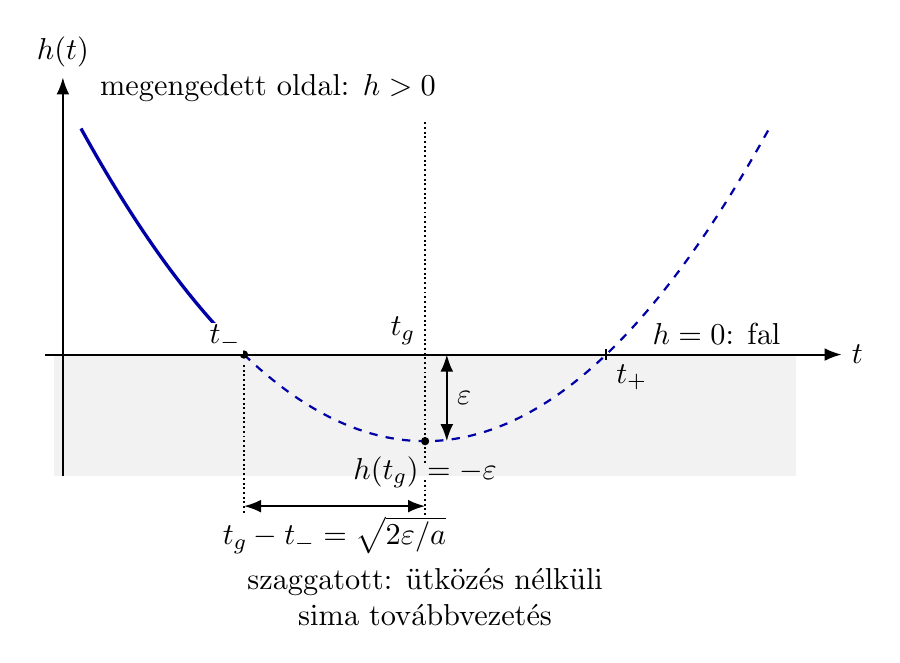
\begin{tikzpicture}[x=2.3cm,y=1.1cm,>=Latex,line width=.7pt,
 font=\normalfont\fontsize{11}{13.2}\selectfont]
\fill[gray!10] (-2.05,-1.4) rectangle (2.05,0);
\draw[->] (-2.1,0)--(2.3,0) node[right] {$t$};
\draw[->] (-2,-1.4)--(-2,3.2) node[above] {$h(t)$};
\node[above right] at (1.2,0) {$h=0$: fal};
\node[above right] at (-1.85,2.8) {megengedett oldal: $h>0$};
\draw[blue!65!black,very thick,domain=-1.9:-1,samples=50]
 plot (\x,{\x*\x-1});
\draw[blue!65!black,thick,dashed,domain=-1:1.9,samples=100]
 plot (\x,{\x*\x-1});
\draw[densely dotted] (0,-1.25)--(0,2.7);
\fill (-1,0) circle (1.5pt); \fill (0,-1) circle (1.5pt);
\draw (1,-.06)--(1,.06);
\node[above left,fill=white,inner sep=1pt] at (-1,0) {$t_-$};
\node[above left] at (0,0) {$t_g$};
\node[below right] at (1,0) {$t_+$};
\draw[<->] (.12,0)--(.12,-1) node[midway,right] {$\varepsilon$};
\node[below] at (0,-1.06) {$h(t_g)=-\varepsilon$};
\draw[densely dotted] (-1,-.12)--(-1,-1.85);
\draw[densely dotted] (0,-1.45)--(0,-1.85);
\draw[<->] (-1,-1.75)--(0,-1.75)
 node[midway,below] {$t_g-t_-=\sqrt{2\varepsilon/a}$};
\node[align=center] at (0,-2.8) {szaggatott: ütközés nélküli\\sima továbbvezetés};
\end{tikzpicture}

\caption{A \eqref{eq:grazing_motivation} lokális parabolaközelítés geometriai jelentése, $\varepsilon>0$ esetén. A folytonos ág a beérkező mozgás; a szaggatott görbe az ütközést figyelmen kívül hagyó folytatás. A szürke tartomány a merev fal esetén nem megengedett.}\label{fig:grazing_parabola}
\end{figure}
A \ref{fig:grazing_parabola}. ábrán a függőleges tengely az előjeles faltávolság, a vízszintes az idő. A parabola minimuma $(t_g,-\varepsilon)$; az $a>0$ a görbületet meghatározó normálgyorsulás. A falat először a bal oldali $t_-$ gyöknél érjük el. A $h=0$ feltételből $(t-t_g)^2=2\varepsilon/a$, ezért az érintési időhöz viszonyított eltérés négyzetgyökösen függ $\varepsilon$-tól. A jobb oldali $t_+=t_g+\sqrt{2\varepsilon/a}$ csak a simán továbbvezetett parabola második gyöke: a tényleges ütköző pálya már $t_-$-nál visszapattan, és onnantól más görbét követ. Ha $\varepsilon=0$, a parabola éppen érinti a falat; $\varepsilon<0$ esetén a minimum is felette marad.

Itt $t_g$ a minimum időpontja, $a$ a helyi normálgyorsulás, $\varepsilon$ pedig az ütközés nélküli pálya legnagyobb behatolása. Ez utóbbi csak a simán továbbvezetett pálya geometriai jellemzője: a merev falon a tényleges pálya nem halad át. Ha $\varepsilon<0$, nincs ütközés; $\varepsilon=0$ a grazing; $\varepsilon>0$ esetén a beérkező ág első falelérése és sebessége vezető rendben
\begin{equation}\label{eq:grazing_motivation_speed}
t_-=t_g-\sqrt{\frac{2\varepsilon}{a}},\qquad
v^-\simeq-\sqrt{2a\varepsilon}.
\end{equation}
A $v^+=-rv^-$ visszapattanási törvény ezért
\begin{equation}\label{eq:grazing_motivation_jump}
\Delta v=v^+-v^-\simeq(1+r)\sqrt{2a\varepsilon}
\end{equation}
sebességugrást eredményez. Például $a=1\,\mathrm{m/s^2}$ és $r=0{,}8$ mellett $\varepsilon=0{,}01\,\mathrm{mm}$ esetén $\Delta v\simeq0{,}00805\,\mathrm{m/s}$; százszor nagyobb behatolás tízszer nagyobb sebességugrást ad. A kapcsolat tehát négyzetgyökös, nem lineáris.

Ha az ütközés utáni mozgást egy rögzített metszetig továbbvezetjük, ez a kis sebességváltozás a visszatérési állapotban is általában $\sqrt{\varepsilon}$ rendű korrekciót okoz. Innen ered a \emph{square-root mapping}. Az együttható és az irány a további mozgástól és a metszettől függ; a fenti helyi számítás még nem a teljes visszatérési leképezés. A korrekció nullához tart, de érzékenysége $\varepsilon\to0^+$ esetén korlátlanná válhat. Ez magyarázza, miért romlik el a szokásos lineáris közelítés a grazing közelében.

Ilyen geometria jelenhet meg hézagos mechanizmusok, ütközővel határolt rezgések vagy egy akadályt éppen elérő periodikus pálya esetén. A következő ütköző oszcillátor ezt a helyzetet modellezi. A levezetés nemelfajuló, merev ütközésre vonatkozik; tartós kontaktushoz vagy $a=0$ érintkezéshez más helyi modell szükséges.


Tekintsük az alábbi rendszert:
\begin{equation}
\dot{x}=F(x), \quad \text{ahol } x\in S^+=\left\{x\in\mathcal{D}\subset\mathbb{R}^n: H(x)>0\right\},
\end{equation}
amely a
\begin{equation}
\Sigma:=\left\{x\in\mathcal{D}: H(x)=0\right\}
\end{equation}
felületen ütközik az
\begin{equation}
x^+=R(x^-):=x^-+W(x^-)v_H(x^-)
\end{equation}
leképezés által kijelölt módon. $H(x)$ a kapcsolóvonal egyenlete, $x^+$ az ütközés utáni állapotváltozó, $x^-$ pedig az ütközés előtti állapotváltozó. Az ütközés pillanatában a kapcsolófelületre merőleges sebességet és gyorsulást a
\begin{equation}
v_H(x)=H_xF(x),
\end{equation}
a gyorsulást pedig
\begin{equation}
 a_H(x)=F(x)^\mathsf T H_{xx}(x)F(x)+H_x(x)F_x(x)F(x)
\end{equation}
összefüggésekkel adjuk meg. Ezek $H$ első és második időderiváltjai; geometriai normálsebességgel csak megfelelően normalizált $H$ esetén azonosak. A $H_{xx}$ Hess-mátrix. A továbbiakban $a_H$-t röviden $a$ jelöli.
\exampleend

\section{1DoF ütköző oszcillátor}
\examplebody

Az ütköző oszcillátor alapmodelljéhez és periodikus mozgásához lásd \cite[1.2.1--1.2.2. és 6.1. szakasz]{dib}.


Az 1 DoF ütköző oszcillátor dimenziótlan egyenlete az alábbi:
\begin{equation}
u''(t)+2\zeta u'(t)+u(t)=w(t),\qquad u(t)>\sigma,\qquad \zeta\geq0.
\end{equation}
A $t=t_0$ (ütközéskori) időpillanatban az alábbi leképezés valósul meg:
\begin{equation}
f(u^-,v^-):=(u^+,v^+),
\end{equation}
ahol közvetlenül az ütközés előtti pozíció és sebesség
\begin{equation}
u^-=u(t_0),
\end{equation}
\begin{equation}
v^-=v(t_0)=\left.\frac{\mathrm{d}u}{\mathrm{d}t}\right|_{t=t_0},
\end{equation}
továbbá a közvetlenül az ütközés utáni pozíció és sebesség felírható az alábbi módon:
\begin{equation}
u^+=u^-,
\end{equation}
\begin{equation}
v^+=-rv^-, \quad 0\le r\le 1.
\end{equation}
Megjegyzés: $1-r^2$ meghatározza az ütközés során elnyelt mozgási energiaarányt. $r$ a különböző anyagok tulajdonságaitól függ, $r$ értékét mérésből vagy kontaktusmodellből kell meghatározni; az ábrákon $r=0{,}95$ egy választott példa. $r=1$ a tökéletesen rugalmas és $r=0$ a tökéletesen rugalmatlan ütközésnek felel meg. Az általunk vizsgált esetben $w(t)=\cos(\omega t)$ a periodikus gerjesztés $\frac{2\pi}{\omega}$ periódussal:
\begin{equation}
u''(t)+2\zeta u'(t)+u(t)=\cos(\omega t),\qquad u>\sigma.
\end{equation}
Az 1DoF ütköző oszcillátor átírható az alábbi három-dimenziós autonóm rendszerré:
\begin{equation}
\begin{split}
\frac{\mathrm{d}u}{\mathrm{d}t}&=v,\\
\frac{\mathrm{d}v}{\mathrm{d}t}&=-u-2\zeta v+w(s),\\
\frac{\mathrm{d}s}{\mathrm{d}t}&=1,
\end{split}\qquad \qquad \text{ha } u>\sigma,
\end{equation}
azaz az alábbi autonóm rendszer adódik. A $w(s)=\cos(\omega s)$ miatt a kibővített rendszer nem lineáris:
\begin{equation}
\dot{x}=F(x),
\end{equation}
ahol
\begin{equation}\label{eq:xFx}
x=\begin{pmatrix}
u\\ v\\ s
\end{pmatrix},\qquad
F(x)=\begin{pmatrix}
v\\
-u-2\zeta v+w(s)\\
1
\end{pmatrix}.
\end{equation}
A kapcsolóvonal egyenlete
\begin{equation}
H(x)=u-\sigma,
\end{equation}
gradiense pedig

\begin{equation}\label{eq:hx}
H_x=\begin{pmatrix}1&0&0\end{pmatrix}.
\end{equation}
A leképezés a kapcsolóvonalon:

\begin{equation}
x \rightarrow R(x)=\begin{pmatrix}
u\\
-r v\\
s,
\end{pmatrix}
\end{equation}
azaz a reset leképezés Jacobi-mátrixa

\begin{equation}\label{eq:Rx}
R_x(x)=\begin{pmatrix}
1 & 0 & 0\\
0 & -r & 0\\
0 & 0 & 1
\end{pmatrix}.
\end{equation}
A sebesség, illetve a gyorsulás az alábbi módon írható le:
\begin{equation}
v_H(x)=v,
\end{equation}
\begin{equation}
a(x)=-u-2\zeta v+w(s),
\end{equation}
így kapcsolóvonalra történő becsapódási sebesség:

\begin{equation}
H_x(x^-) F(x^-) = v^-,
\end{equation}
Újra megemlítjük a \eqref{eq:Qxmatrix} egyenletre levezetett korrekciós mátrixot:

\begin{equation}\label{eq:Qxmatrix2}
Q_x(x^-)=R_x(x^-)+\frac{F(R(x^-))-R_x(x^-)F(x^-)}{H_x(x^-)F(x^-)}H_x(x^-)\,,
\end{equation}
ahol $x^-$ legyen egy periodikus pálya ütközési pontja. Felhasználva, hogy
\begin{equation}
x^+=R(x^-),
\end{equation}
azaz az ütközés utáni állapot felírható az ütközés előtti állapot és leképezés segítségével. \eqref{eq:xFx}, \eqref{eq:hx}, \eqref{eq:Rx} egyenletek felhasználásával:

\begin{equation}
\begin{split}
Q_x(x^-)=\begin{pmatrix}
1 & 0 & 0\\
0 & -r & 0\\
0 & 0 & 1
\end{pmatrix}+\frac{\left(F(x^+)-R_x(x^-)F(x^-)\right)H_x}{v^-}=\\
=\begin{pmatrix}
1 & 0 & 0\\
0 & -r & 0\\
0 & 0 & 1
\end{pmatrix}+\frac{1}{v^-}\left(\begin{pmatrix}
v^+-v^-\\
a^++ra^-\\
1-1
\end{pmatrix} \right)H_x=\begin{pmatrix}
-r & 0 & 0\\
\frac{a^++ra^-}{v^-} & -r & 0\\
0 & 0 & 1
\end{pmatrix}.
\end{split}
\end{equation}

A \ref{fig:phase}--\ref{fig:ut}. ábrák ugyanannak a három numerikus megoldásnak két nézetét mutatják. Mindhárom esetben $\sigma=0$, $r=0{,}95$, $\zeta=0$, a kezdeti állapot $u(0)=1$, $v(0)=0$, a gerjesztés pedig $\cos(\omega t)$. A frekvenciák rendre $\omega=3$, $2{,}76$ és $2{,}9$. A $T=2\pi/\omega$ gerjesztési periódussal mérve $100T$ ideig számoltunk, és az utolsó tizenkét periódust, a $[88T,100T]$ ablakot ábrázoljuk. Az elhagyott kezdeti szakasz csökkenti a kezdeti feltétel hatását; ez önmagában nem bizonyítja, hogy a megmaradó mozgás periodikus vagy már teljesen állandósult.

A szabad mozgás szakaszai a csillapítatlan egyenlet pontos megoldásából származnak; az $u=0$ eseményidőket gyökkereséssel határoztuk meg, majd a $v^+=-rv^-$ reset leképezést alkalmaztuk. A reprodukálható ábragenerátor a \texttt{codes/impact\_figures\_v3.py}; a rövid MATLAB-példa a \texttt{codes/impact\_portraits\_v3.m}, amely az \ref{ap:codes1}. függelék eseményvezérelt integrátorát használja.

\begin{figure}[p]
\centering
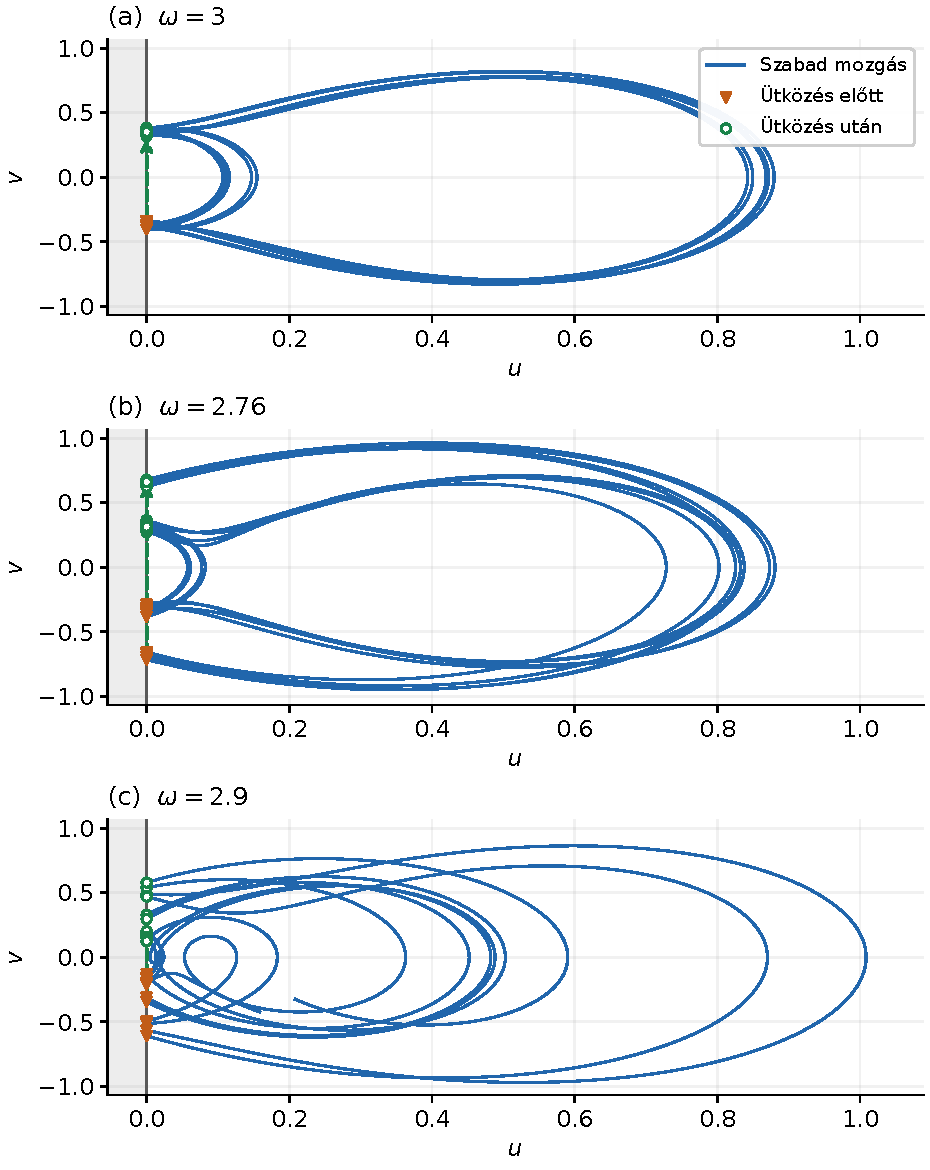
\includegraphics[width=.95\linewidth]{graphics_v3/impact_phase.pdf}
\caption{Az ütköző oszcillátor $(u,v)$ fázissíkbeli vetülete három frekvencián, azonos tengelyskálákkal. Kék: szabad mozgás; narancssárga háromszög: ütközés előtti állapot; zöld üres kör: ütközés utáni állapot. A fal $u=0$, a szürke oldal nem megengedett. Panelenként egy szaggatott nyíl szemlélteti a sebességugrást.}\label{fig:phase}
\end{figure}


A \ref{fig:phase}. ábrán a vízszintes koordináta az elmozdulás, a függőleges a sebesség. A $v<0$ ágakon a tömeg a fal felé halad, a $v>0$ ágakon távolodik tőle; a $v=0$, $u>0$ pontok a kitérés fordulópontjai. A falat a pálya $(0,v^-)$ pontban éri el, majd ugyanazon helyen $(0,-rv^-)$ állapotból folytatódik. Az ezt összekötő szaggatott nyíl pillanatszerű állapotugrást jelöl, nem a szabad mozgás egy szakaszát. A kisebb visszapattanási sebesség miatt az ütközés utáni jel közelebb van a $v=0$ tengelyhez, mint a hozzá tartozó beérkező jel.

Az ismételten bejárt ívek egymásra rajzolódhatnak, ezért egyetlen látható ív több időbeli bejárást is takarhat. A különböző falelérési sebességek eltérő ütközési állapotokat jeleznek. Fontos, hogy ez a háromdimenziós $(u,v,s)$ rendszer kétdimenziós vetülete: azonos $(u,v)$ ponton különböző gerjesztési fázisokban is áthaladhat a megoldás. A vetületi kereszteződés ezért nem sérti a megoldás egyértelműségét. A bonyolultabb vonalrajz önmagában nem bizonyít káoszt; ehhez például Poincaré-metszetet vagy Ljapunov-exponenst kell vizsgálni.

\begin{figure}[p]
\centering
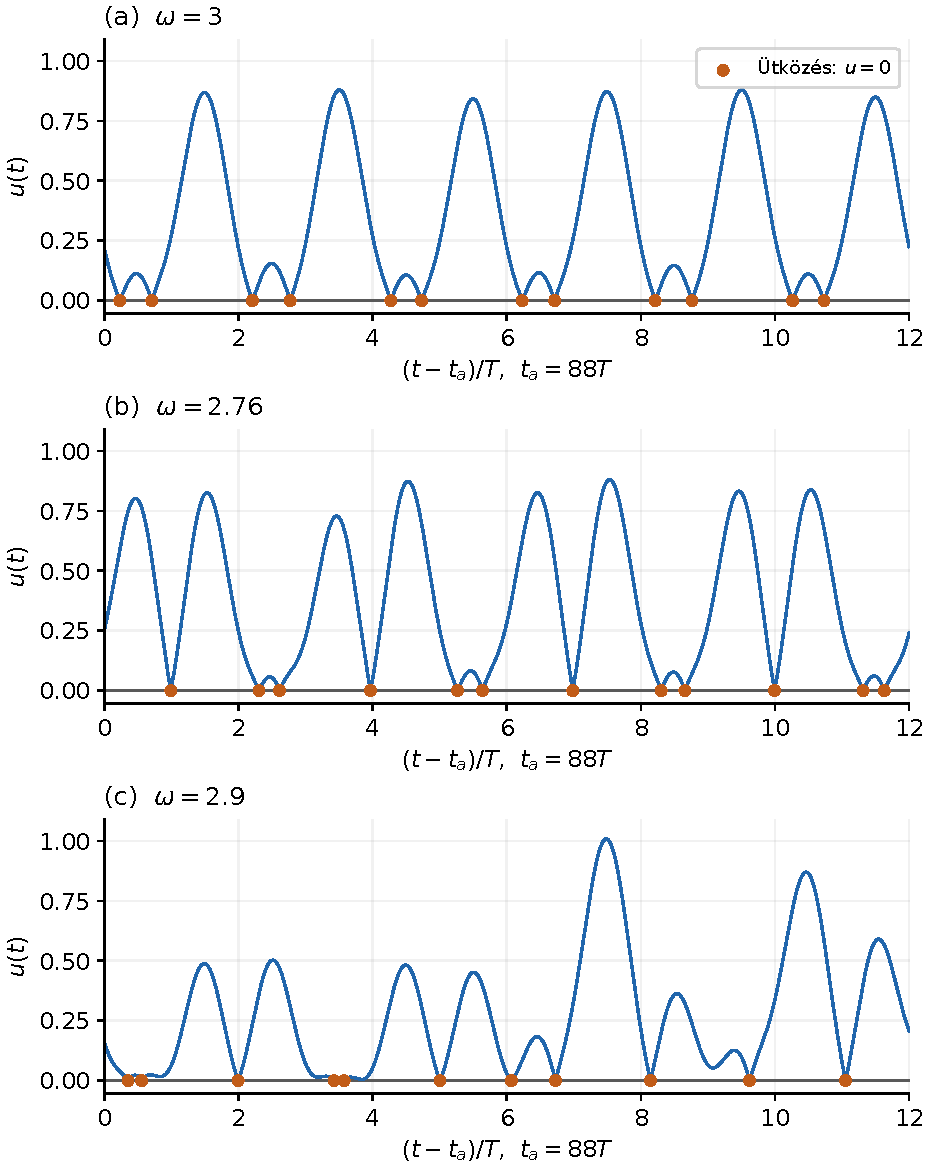
\includegraphics[width=.95\linewidth]{graphics_v3/impact_time.pdf}
\caption{A \ref{fig:phase}. ábra pályái az időtartományban, azonos elmozdulásskálával. A vízszintes tengely a $t_a=88T$ időponttól eltelt gerjesztési periódusok száma. A narancssárga pontok az ütközéseket jelölik; a folytonos elmozdulásgörbe meredeksége ekkor ugrik.}\label{fig:ut}
\end{figure}


A \ref{fig:ut}. ábra megmutatja az ütközések sorrendjét és a köztük eltelt időt, amit a fázisábrán az egymásra rajzolódó ívek elfedhetnek. Minden narancssárga pontban $u=0$, de a test nem halad a fal mögé. A kitérés folytonos marad, miközben a bal oldali meredekség $v^-<0$ értékről a jobb oldali $v^+=-rv^->0$ értékre ugrik: ezért látható csúcsos minimum az ütközésnél. A falhoz csak kis sebességgel érkező pályának kisebb a meredekségugrása; a grazing határesetben $v^-=0$ és az érintés simává válhat.

A megjelenített ablakban az (a) panelen közel ismétlődő nagy és kis kitérések váltakoznak; a (b) panelen a nagy kitérések közé kis, fal közeli visszapattanások ékelődnek; a (c) panelen a csúcsmagasságok és az ütközési időközök változatosabbak. Ezek a választott véges időablak megfigyelései, nem a mozgások bizonyított dinamikai osztályozása. A hosszú idejű részletes ütközéssor érzékeny lehet a numerikus kerekítésre; a két ábra ugyanazon számítás adatait használja.

A panelek összevetésével a csúcskitérések és az ütközések közti idő változását lehet leolvasni. Egy vízszintes egység minden panelben egy gerjesztési periódus, de eltérő $\omega$ mellett eltérő fizikai időt jelent. A $\zeta=0$ választás csak a folytonos viszkózus csillapítást kapcsolja ki: az $r<1$ ütközési törvény továbbra is energiát veszít, amelyet a gerjesztés részben pótolhat.

A mátrixok a \emph{perturbációkat}, nem magukat az állapotokat képezik le. Ha a periódus egy folytonos szakasszal és annak végén egy ütközéssel írható le, akkor
\[
\delta x^- = M\delta x_0,\qquad
\delta x^+ = Q_x\delta x^-,\qquad
\mathcal M=Q_xM.
\]
Általában a folytonos szakaszok variációs mátrixait és az események korrekciós mátrixait időrendi sorrendben kell összeszorozni; az időben későbbi tényező balra kerül. A $3\times3$ autonóm leírásból rögzített gerjesztési fázisnál a $2\times2$ állapotérzékenységet használjuk. A továbbiakban az ütközési képletben $Q_x$ ezt a kétdimenziós blokkot jelenti.
\exampleend

\section{Ütközés nélküli eset -- monodrómia-mátrix}
Tegyük fel, hogy $\left(u(t),v(t)=\frac{\mathrm{d}u}{\mathrm{d}t}\right)$ megoldása a
\begin{equation}
u''(t)+2\zeta u'(t)+u=w(t)
\end{equation}
egyenletnek. Tekintsük az alábbi perturbált megoldást: $\left(u(t)+\delta u(t),v(t)+\delta v(t)\right)$. A $\delta u$ függvény kielégíti az alábbi variációs egyenletet
\begin{equation}
\delta u''(t)+2\zeta \delta u'(t)+\delta u=0,\qquad \left(\delta u(t_0),\delta v(t_0) \right)=\left(\delta u_0,\delta v_0 \right),
\end{equation}
azaz
\begin{equation}
\frac{\mathrm{d}}{\mathrm{d}t}\begin{pmatrix}
\delta u\\ \delta v
\end{pmatrix}=L\begin{pmatrix}
\delta u\\ \delta v
\end{pmatrix}:=\begin{pmatrix}
0 & 1 \\
-1 & -2\zeta
\end{pmatrix}\begin{pmatrix}
\delta u\\ \delta v
\end{pmatrix}.
\end{equation}
Így felírható az egy $(T)$ periódusra vonatkozó állapotvektor variációja:
\begin{equation}
\begin{pmatrix}
\delta u_T\\ \delta v_T
\end{pmatrix}:=
\begin{pmatrix}
\delta u(t_0+T)\\
\delta v(t_0+T)
\end{pmatrix}
=\mathrm{e}^{LT}\begin{pmatrix}
\delta u(t_0)\\ \delta v(t_0)
\end{pmatrix}.
\end{equation}
Így az egy periódusra vonatkozó leképezés (monodrómia) mátrixa
\begin{equation}\label{eq:Nt}
N_T=\mathrm{e}^{LT}=\mathrm{e}^{-\zeta T}
\begin{pmatrix}
C_T+\zeta S_T/\omega_0 & S_T/\omega_0\\
-S_T/\omega_0 & C_T-\zeta S_T/\omega_0
\end{pmatrix},
\end{equation}
ahol az alulcsillapított, $0\leq\zeta<1$ esetben
\[
\omega_0=\sqrt{1-\zeta^2},\qquad C_T=\cos(\omega_0T),\qquad S_T=\sin(\omega_0T).
\]
Ellenőrzésként $N_0=I$ és $\left.\frac{dN_T}{dT}\right|_{T=0}=L$. A kritikus esetben ($\zeta=1$) $S_T/\omega_0$ határértéke $T$, $C_T$ határértéke $1$. Túlcsillapításnál $\beta=\sqrt{\zeta^2-1}$ bevezetésével $C_T=\cosh(\beta T)$ és $S_T/\omega_0=\sinh(\beta T)/\beta$ helyettesítendő. A $\mathrm{e}^{LT}$ alak minden esetben érvényes.
Érdemes megemlíteni, hogy
\begin{equation}
\det\left(N_T \right)=\mathrm{e}^{-2\zeta T},
\end{equation}
azaz a rendszer disszipatív, ha $\zeta>0$.

\section{Ütközéses eset -- korrekciós mátrix}

Tegyük fel, hogy a $T$ időintervallumban ütközés történik a $t=t_0+t_I$ időpillanatban. Az ütközés előtti sebesség $v_I<0$, az ütközés előtti gyorsulás $a_I^-$, az ütközés utáni gyorsulás pedig $a_I^+$. A mozgás dinamikáját módosítja az ütközés, ennek leírásához pedig a $Q_x$ mátrix kerül kiszámításra (\eqref{eq:Qxmatrix2} egyenlet). Így a $T$ periódusra vonatkozó állapotvektor-variáció az alábbi módon írható le:
\begin{equation}
\begin{pmatrix}
\delta u_T\\ \delta v_T
\end{pmatrix}:=
\begin{pmatrix}
\delta u(t_0+T)\\
\delta v(t_0+T)
\end{pmatrix}
=\tilde{N}_T\begin{pmatrix}
\delta u_0\\ \delta v_0
\end{pmatrix},
\end{equation}
ahol $\tilde{N}_T$ (\eqref{eq:Nt} egyenlet felhasználásával) az alábbi módon számolható:
\begin{equation}
\tilde{N}_T=N_{T-t_I}Q_xN_{t_I}.
\end{equation}
Jelen esetben $\tilde{N}_T$ determinánsa
\begin{equation}
\det\left( \tilde{N}_T\right)=\mathrm{e}^{-2\zeta T}r^2.
\end{equation}
Általánosítva ($m$ ütközés történik a $T$ periódus alatt):
\begin{equation}
\det\left(\tilde{N}_T \right)=\mathrm{e}^{-2\zeta T}r^{2m}.
\end{equation}
$T>0$, $0<r\leq1$ és $\zeta\geq0$ mellett a periódustérkép területet csökkent, ha $\zeta>0$, vagy ha $m\geq1$ és $r<1$. Ez nem garantálja a pálya stabilitását: a determináns a multiplikátorok szorzatát adja, nem az egyes abszolút értékeket. A transzverzális képletekhez minden ütközésnél $v^-\neq0$ szükséges.

\section{Poincaré-leképezés linearizálása}
Legyen $\pi(x)=0$ egy lokális metszet, $n^\mathsf T=\pi_x(x_p)$ és $n^\mathsf TF(x_p)\neq0$. A közös időpontban számított perturbációt az eseményidő változása miatt a metszetre kell vetíteni. Ha $\mathcal M$ az egy periódusra számított teljes variációs mátrix, akkor a metszet érintőterén
\begin{equation}\label{eq:poincare_projection}
DP=\left(I-\frac{F(x_p)n^\mathsf T}{n^\mathsf TF(x_p)}\right)\mathcal M.
\end{equation}
A jobb oldali operátort a metszet kezdeti és végső koordinátáira kell megszorítani; a teljes $n\times n$ mátrixot nem tekintjük $(n-1)$ dimenziós leképezésnek.

Az oszcillátor $v=0$ metszetén $n^\mathsf T=(0,1,0)$, és a transzverzalitás feltétele $a_0\neq0$. A metszet koordinátái $(u,s)$, ahol $s$ a gerjesztési fázis modulo $2\pi/\omega$. A referencia-periódushoz közeli visszatérési idő eltolódása $\delta\tau=-\delta v/a_0$. Így az időkoordináta korrigálódik, miközben $v=0$ miatt az $u$ koordináta első rendben nem változik az időkorrekciótól. A vetítés transzverzális eseményekkel tagolt pályára is alkalmazható, ha $\mathcal M$ már tartalmazza a saltation-mátrixokat.

\section{Reguláris grazing és a négyzetgyök eredete}
A helyi geometria és a discontinuity mapping típusú leképezések részletes könyvbeli tárgyalása: \cite[2.5.3. és 6.2--6.3. szakasz]{dib}.

A $H>0$ megengedett tartomány felől nézve a reguláris grazing feltételei:
\[
H(x^*)=0,\qquad H_x(x^*)F(x^*)=0,\qquad a_H(x^*)>0,\qquad H_x(x^*)\neq0.
\]
Az utolsó előtti feltétel a nemelfajuló lokális minimumot biztosítja. A kontaktus közelében az ütközés nélkül továbbvezetett sima megoldásra
\[
H(x(t))=h_{\min}+\frac12a_H(x^*)(t-t_g)^2+\cdots.
\]
Ha $h_{\min}<0$, az eseményidő eltérése vezető rendben $|t-t_g|\sim\sqrt{-2h_{\min}/a_H(x^*)}$. Innen származik az ütközés utáni visszatérési leképezés négyzetgyökös tagja; a leképezés általában nem differenciálható a grazing-határon \cite{nordmark}.

Lokális koordinátákban legyen $\xi=0$, $\mu=0$ a referenciapont, és $P_0(\xi,\mu)=N\xi+B\mu$ a sima visszatérés elsőrendű része. A legkisebb távolság elsőrendű modelljét jelölje
\[
h(\xi,\mu)=c^\mathsf T(N\xi+B\mu)+d_h\mu.
\]
A $h$ nem a metszetben vett pillanatnyi $H$-érték, hanem a továbbvezetett pálya kontaktushoz viszonyított minimális távolságának lokális modellje. A vezető rendű, csonkolt Nordmark-típusú leképezés:
\begin{equation}\label{eq:nordmark}
P_N(\xi,\mu)=\begin{cases}
N\xi+B\mu+E\sqrt{-h(\xi,\mu)},& h(\xi,\mu)<0,\\
N\xi+B\mu,& h(\xi,\mu)\geq0.
\end{cases}
\end{equation}
A dimenziók: $\xi,E,c\in\mathbb R^d$, $N\in\mathbb R^{d\times d}$, $B\in\mathbb R^{d\times1}$ és $d_h\in\mathbb R$. A koefficienseket a sima dinamika, a kontaktus és a választott koordináták határozzák meg; \eqref{eq:nordmark} nem egy globálisan pontos linearizálás.

\section{Fixpontok és admissibility}
Ha $I-N$ invertálható, a sima ág fixpontjelöltje
\[
\xi_e=(I-N)^{-1}B\mu.
\]
Ez csak $h(\xi_e,\mu)\geq0$ esetén fixpontja a teljes csonkolt leképezésnek. Az ütköző ágon a
\[
(I-N)\xi=B\mu+E\sqrt{-h(\xi,\mu)},\qquad h(\xi,\mu)<0
\]
egyenletet kell megoldani. Az ágfeltételt egy gyökvonás utáni négyzetre emeléskor is meg kell őrizni. Az ütköző ágon
\[
D_\xi P_N=N-\frac{E c^\mathsf TN}{2\sqrt{-h(\xi,\mu)}};
\]
a multiplikátorok ebből, a sima ágon $N$-ből adódnak.

A $z=\xi-\xi_e$, $\chi=-h(\xi_e,\mu)$ eltolás a csonkolt modellben
\[
z\mapsto\begin{cases}
Nz+E\sqrt{\chi-c^\mathsf TNz},&c^\mathsf TNz<\chi,\\
Nz,&c^\mathsf TNz\geq\chi.
\end{cases}
\]
A $\chi$ lokális paraméter, nem az oszcillátor $\sigma$ falhelyzete.

\section{Egydimenziós szemléltető modell}
\examplebody

A skaláris modell és a többdimenziós square-root mapping típusú leképezések kapcsolatához lásd \cite[1.4.2. és 4.3. szakasz]{dib}.

Egy általános többdimenziós Nordmark-leképezés nem redukálható egyetlen legnagyobb sajátérték alapján skaláris rendszerre: a négyzetgyökös tag nemlineáris és irányokat csatolhat össze. Egydimenziós redukcióhoz külön invariancia- vagy elhanyagolhatósági feltevések és a redukció hibájának becslése szükséges. Az alábbi rendszer ezért önálló szemléltető modell:
\begin{equation}\label{eq:sr}
w_{k+1}=f(w_k)=\begin{cases}
\nu w_k+\sqrt{\mu-w_k},&w_k<\mu,\\
\nu w_k,&w_k\geq\mu,
\end{cases}\qquad 0<\nu<1.
\end{equation}
A két ág $w=\mu$-nél folytonosan illeszkedik, de a bal oldali derivált nem korlátos. Ha $\mu\leq0$, a $w=0$ fixpont a sima ágon van; $\mu<0$ esetén lokálisan aszimptotikusan stabil. Ha $\mu>0$, az ütköző ág fixpontja
\[
w_* = \frac{2\mu}{1+\sqrt{1+4(1-\nu)^2\mu}},\qquad
f'(w_*)=\nu-\frac{1}{2\sqrt{\mu-w_*}}.
\]
Ekkor $0<w_*<\mu$; stabilitását $|f'(w_*)|<1$ dönti el. A $\mu=0$ határpontot a sima ág deriváltjából önmagában nem osztályozzuk.

A \ref{fig:square-root}. ábra a két ágat és néhány iterációt mutatja. A görbe és a $w_{k+1}=w_k$ átló közötti váltott függőleges és vízszintes vetítéssel kapjuk a cobweb diagramot.

\begin{figure}[ht!]
\centering
\begin{subfigure}[b]{0.48\linewidth}
         \centering
         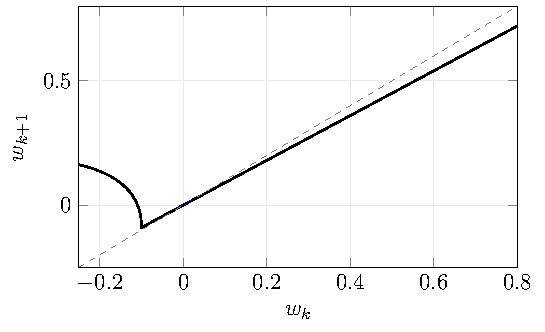
\includegraphics[width=1\linewidth]{graphics_v3/sr_m01.pdf}
         \caption{$\mu=-0.1$}
         \label{fig:s_m01}
     \end{subfigure}
     \begin{subfigure}[b]{0.48\linewidth}
         \centering
         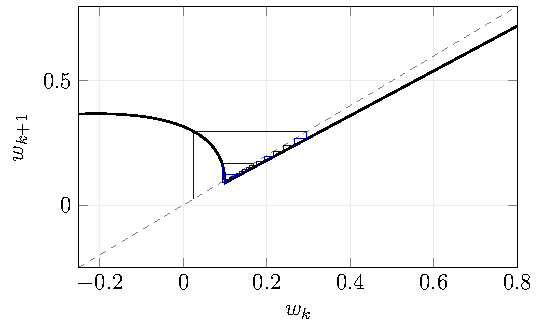
\includegraphics[width=1\linewidth]{graphics_v3/sr_01.pdf}
         \caption{$\mu=0.1$}
         \label{fig:s_01}
     \end{subfigure}
     \caption{Egy dimenziós square-root map különböző $\mu$ értékekre $\nu=0,9$ esetén}\label{fig:square-root}
\end{figure}

A \ref{fig:bif}. ábra rögzített $\nu$ mellett változó $\mu$-höz tartozó, tranziens utáni iterátumokat mutat. A különböző periódusú ablakok és a rendezetlen ponthalmazok a \emph{ciklusok periódusáról}, nem az egyensúlyi helyek számáról adnak információt. Kaotikusság megállapításához például pozitív legnagyobb Ljapunov-exponenst és numerikus konvergenciát is vizsgálni kell. A $\nu$ itt a leképezés sima ágának kontrakciós paramétere; nem azonos közvetlenül a mechanikai csillapítási tényezővel. A korábban megadott $1/4$ és $2/3$ határokat külön levezetés nélkül nem használjuk általános osztályozási tételként.

Az ábrák újraszámolhatók a \texttt{codes/square\_root\_figures\_v3.py} programmal. A bifurkációs mintavételben minden paraméterértéknél azonos kezdeti állapotból indulunk; több együtt létező attraktor teljes feltérképezéséhez több kezdeti állapot szükséges.

\begin{figure}[ht!]
\centering
\begin{subfigure}[b]{0.48\linewidth}
         \centering
         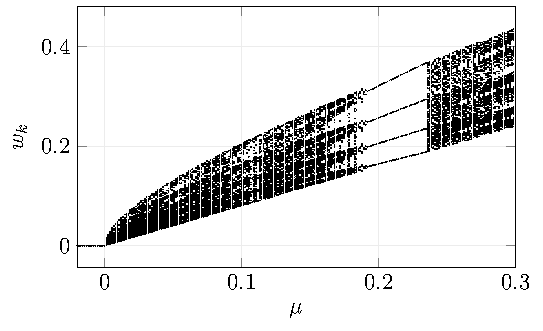
\includegraphics[width=1\linewidth]{graphics_v3/bif_08.pdf}
         \caption{$\nu=0.8$}
         \label{fig:kis_csillapitas}
     \end{subfigure}
     \begin{subfigure}[b]{0.48\linewidth}
         \centering
         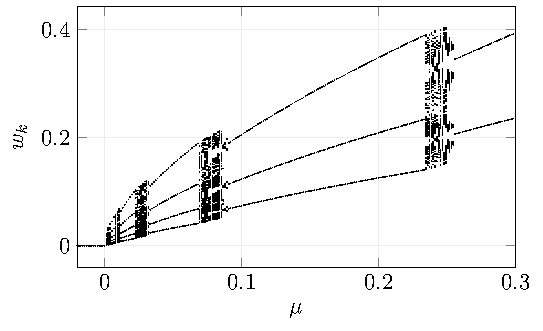
\includegraphics[width=1\linewidth]{graphics_v3/bif_06.pdf}
         \caption{$\nu=0.6$}
         \label{fig:kozepes_csillapitas}
     \end{subfigure}
     \begin{subfigure}[b]{0.48\linewidth}
         \centering
         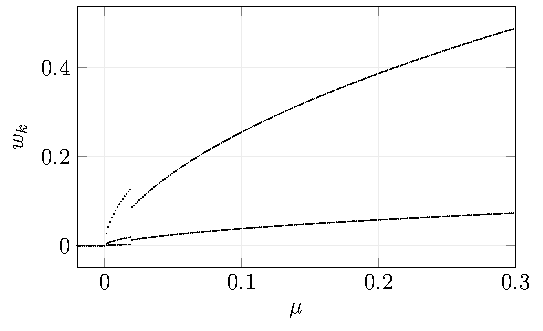
\includegraphics[width=1\linewidth]{graphics_v3/bif_015.pdf}
         \caption{$\nu=0.15$}
         \label{fig:nagy_csillapitas}
     \end{subfigure}
     \caption{Bifurkációs diagram az 1D square-root mapra vonatkozóan különböző $\nu$ értékek esetén (bifurkációs paraméter: $\mu$)}\label{fig:bif}
\end{figure}

\newpage
\exampleend


%!TEX root = ../SzFDR_jegyzet_v3.tex

\chapter{\label{sec:perpalyakovetes}Periodikus pályák numerikus követése}

Dinamikai rendszerek vizsgálatánál kíváncsiak vagyunk a rendszer viselkedésére különböző paraméterkombinációk esetében is.
A paraméterek ha\-tá\-sá\-nak vizsgálatára többféle módszer is rendelkezésünkre áll, mint például a paraméterléptetés vagy a pseudo-arclength continuation eljárás.
Paraméterléptetés esetén a bifurkációs paraméter értékét kis mértékben megváltoztatjuk, ekkor jól megfogalmazott probléma esetén a megoldás is kis mértékben fog változni, és ezt a változást követjük lépésről-lépésre.
Pseudo-arclength continuation esetén a bifurkációs paraméter és a periodikus pálya periódusidejének össze\-füg\-gé\-sét keressük oly módon, hogy a problémát egy "szintvonal" keresésre vezetjük vissza.
A fejezetben ez utóbbival fogunk részletesebben foglalkozni. 

\section{Pseudo-arclength continuation}
A pályakövetés könyvbeli összefoglalása: \cite[2.6.2. szakasz]{dib}; az egyensúlyok és ciklusok numerikus folytatása részletesen: \cite[10.1.4. és 10.2.1. szakasz]{kuznetsov_book}.

\label{sec:pseudo_ivhossz}

A pseudo-arclength continuation eljárás a megoldásgörbét követi, ezért a fizikai paraméter is ismeretlen. A következő pontot egy érintőirányú prediktorhoz tartozó merőleges síkban keressük. A síkbeli $F(\mathbf x)=0$ görbén, egységnyi $\mathbf v_i$ érintővel:
\begin{equation}
\begin{cases}
0 = \left< \mathbf{x}_{i+1} - \mathbf{x}_i, \mathbf{v}_i \right> - \Delta s \\
0 = F(\mathbf{x}_{i+1}),
\end{cases}
\label{eq:pszeudo_ivhossz_alapegyenlet}
\end{equation}
\begin{equation}
\mathbf{x_i}= \begin{bmatrix}
x_i & y_i
\end{bmatrix}^\mathrm{T},
\end{equation}
és $\Delta s$ a prediktor lépéshossza. Ez a valódi ívhosszt csak közelíti.
Az első egyenlet a merőlegességi feltétel, a második magának a keresett szintvonalnak az egyenlete.
A módszer egy iterációs lépésének szemléltetése a \ref{fig:pszeudo_ivhossz_szemleltet}. ábrán látható.
A merőlegességi feltétel az alábbi módon vezethető le:
\begin{equation}
\hat{\mathbf{x}} = \mathbf{x}_i + \Delta s \, \mathbf{v}_i,
\end{equation}
\begin{equation}
\begin{matrix}
\left< \mathbf{x}_{i+1} - \hat{\mathbf{x}}, \mathbf{v}_i \right> & = &
\left< \mathbf{x}_{i+1} - \mathbf{x}_i - \Delta s \, \mathbf{v}_i, \mathbf{v}_i \right>  & = \\
\left< \mathbf{x}_{i+1} - \mathbf{x}_i, \mathbf{v}_i \right> - \Delta s \, \left< \mathbf{v}_i , \mathbf{v}_i \right> & = & \left< \mathbf{x}_{i+1} - \mathbf{x}_i, \mathbf{v}_i \right> - \Delta s. & \blacksquare
\end{matrix}
\end{equation}

\begin{figure}[ht]
	\centering
	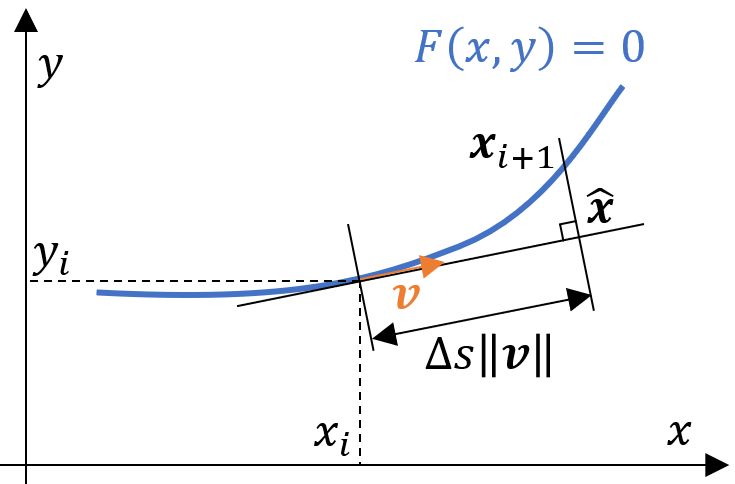
\includegraphics[width=.62\linewidth,trim={0.000bp 0.000bp 0.500bp 1.500bp},clip]{graphics/pszeudo_ivhossz_szemleltet.png}
	\caption{A pseudo-arclength continuation eljárás egy iterációs lépésének szemléltetése}\label{fig:pszeudo_ivhossz_szemleltet}
\end{figure}

A módszer alkalmazása során a \eqref{eq:pszeudo_ivhossz_alapegyenlet} egyenletrendszert szimultán kell megoldani $\mathbf{x}_{i+1}$-re - két egyenlet, két ismeretlen.
A módszer általánosítható több dimenzióra is, ekkor több $F_j(\mathbf{x})$ egyenletre van szük\-sé\-günk.

\exampleheading{Példa: körív követése.}
Akkor az implicit függvényünk az alábbi:
\begin{equation}
F(\mathbf{x}) = x^2 + y^2 -1.
\end{equation}
A kezdőpontunk legyen
\begin{equation}
\mathbf{x}_0 = \begin{bmatrix}
1 & 0
\end{bmatrix}^\mathrm{T},
\end{equation}
amely, mint látható kielégíti az implicit egyenletünket.
A sebességvektor, azaz az érintő ebben a pontban
\begin{equation}
\mathbf{v}_0 = \begin{bmatrix}
0 & 1
\end{bmatrix}^\mathrm{T}.
\end{equation}
Azonban az esetek többségében ez nem ilyen egyszerűen meghatározható, és numerikusan kell közelítenünk, amihez ismernünk kell a szintvonal egy másik, közeli pontját is, $\mathbf{x}_{1/2}$-et:
\begin{equation}
\mathbf{v}_0 = \frac{\mathbf{x}_{1/2} - \mathbf{x}_{0}}{\left \| \mathbf{x}_{1/2} - \mathbf{x}_{0} \right \|}.
\end{equation}
A sebességvektor ezek után rendre:
\begin{equation}
\mathbf{v}_i = \frac{\mathbf{x}_{i} - \mathbf{x}_{i-1}}{\left \| \mathbf{x}_{i} - \mathbf{x}_{i-1} \right \|}.
\end{equation}
A körív követésének eredménye a pseudo-arclength continuation eljárással a \ref{fig:pszeudo_ivhossz_koriv}. ábrán látható.
A lépéshossz $\Delta s = 0.1$ volt, a kezdeti sebességbecsléshez az $\mathbf{x}_0$-hoz közeli szintvonal pont pedig
\begin{equation}
\mathbf{x}_{1/2} = \begin{bmatrix}
0.99 & \sqrt{1 - 0.99^2}
\end{bmatrix}^\mathrm{T}.
\end{equation}

\begin{figure}[ht]
	\centering
	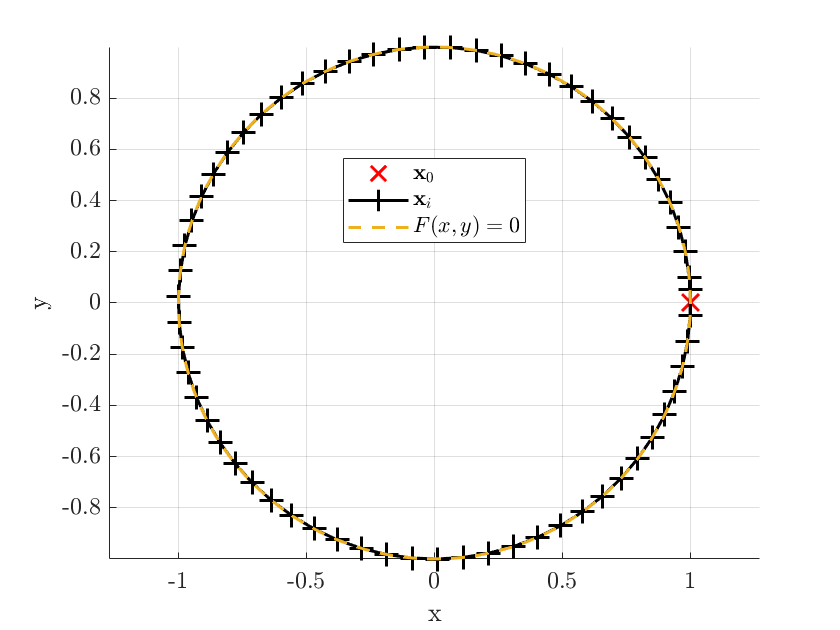
\includegraphics[width=\linewidth,trim={22.497bp 3.000bp 56.243bp 22.497bp},clip]{graphics/pszeudo_ivhossz_koriv.png}
	\caption{A pseudo-arclength continuation eljárás alkalmazása körív követésére}\label{fig:pszeudo_ivhossz_koriv}
\end{figure}
\exampleend

\paragraph*{Érintő, skálázás és lépésvezérlés.}
Az érintő közvetlenül is számítható $DF(\mathbf x_i)\mathbf v_i=0$, $\|\mathbf v_i\|=1$ alapján; orientációját az előző érintővel pozitív skalárszorzat rögzíti. A szekánsirány olcsó közelítés. Különböző mértékegységű változóknál először skálázni kell a koordinátákat, vagy súlyozott skalárszorzatot használni. Sikertelen Newton-korrekciónál csökkentjük a lépéshosszt. A korrekció során a korábbi megoldás és az érintő változatlan; csak elfogadott lépés után frissítjük őket.

A melléklet \texttt{pal\_corrector\_v3.m} függvénye az egész kibővített egyenletrendszert oldja meg, egy érintőkomponenssel sem oszt. Körön például $G(y)=y_1^2+y_2^2-1$ használható. Az általános $G:\mathbb R^q\to\mathbb R^{q-1}$ reziduum lehet egy diszkretizált peremfeladat is.

\FloatBarrier
\exampleheading{Példa: áthaladás egy visszahajláson.}
A $\dot x=\mu-x^2$ rendszer egyensúlyai $G(x,\mu)=\mu-x^2=0$ görbét alkotnak. $\mu>0$ mellett az $x=+\sqrt\mu$ ág stabil, az $x=-\sqrt\mu$ ág instabil; $\mu=0$-nál találkoznak. A $\mu$ szerinti egyirányú léptetés itt megakad, míg a pseudo-arclength continuation eljárás átjut az $x=0$ ponton. A függelékben közölt rövid program közvetlenül a melléklet korrektorát használja, globális változók nélkül. A két kezdőpont ismert egyensúly; minden új pontot a két előzőből számítunk.
\phantomsection\label{use:fold}A teljes MATLAB-program az A függelék \ref{ap:fold}. szakaszában található (\pageref{ap:fold}. oldal).
\exampleend

\section{Közönséges differenciálegyenletek peremérték-feladatai}

A \emph{peremérték-feladat} (angolul: \emph{Boundary Value Problem}, röviden BVP) olyan közönséges differenciálegyenlet vagy egyenletrendszer megoldását keresi, amelyre a keresett függvény az integrálási tartomány \emph{mindkét végpontjában} megadott feltételeknek kell, hogy eleget tegyen.

Legyen adott egy $n$-edrendű közönséges differenciálegyenlet az ismeretlen $y(x)$ függvényre:
\[
F\big(x, y, y', y'', \ldots, y^{(n)}\big) = 0,
\qquad x \in [a,b].
\]
Szeparált peremfeltételek az alábbi alakban adhatók meg; a periodikus feltételek a két végpontot közvetlenül összekapcsolják:
\[
B_a\big(y(a), y'(a), \ldots, y^{(n-1)}(a)\big) = 0,
\qquad
B_b\big(y(b), y'(b), \ldots, y^{(n-1)}(b)\big) = 0,
\]
ahol $B_a$ és $B_b$ a bal és jobb határpontban előírt feltételeket jelölik.

\begin{itemize}
\item A \emph{kezdeti érték feladat} (IVP) esetén a megoldás és annak származtatott értékei egyetlen pontban (általában $x=a$-ban) ismertek. Amennyiben a feladat korrekt kitűzésű, a megoldás létezése és egyértelműsége biztosított.
\item A \emph{peremérték-feladat} ezzel szemben olyan feladat, ahol az előírt feltételek különböző pontokban (pl. $x=a$ és $x=b$) adottak. A BVP tehát tipikusan „kétponti” feltételrendszert jelent, de többpontos általánosítás is lehetséges. Egy BVP-nek lehet nulla, egyetlen, több véges számú vagy végtelen sok megoldása.
\end{itemize}

\subsection{Megoldási módszerek}

A peremérték-feladatok többsége nem oldható meg analitikusan, ezért numerikus módszereket alkalmazunk. A leggyakrabban használt eljárások:

\begin{itemize}
  \item \textbf{Shooting módszer:}
  A BVP-t kezdeti érték feladattá alakítja úgy, hogy az ismeretlen kezdeti feltételeket iteratív módon módosítja, amíg a jobb oldali peremfeltétel teljesül.

  \item \textbf{Multiple shooting módszer:}
  A tartományt több szakaszra osztja, és minden szakaszon külön IVP-t old meg, majd a megoldásokat illeszti össze a csatlakozási feltételek alapján.

  \item \textbf{Kollokációs módszerek:}
  A keresett megoldást közelítő függvények (pl. polinomok, spline-ok) lineáris kombinációjaként írják fel, és az egyenletet diszkrét pontokban kényszerítik teljesülni.

  \item \textbf{Véges differencia (finite difference) módszer:}
  Az egyenletet differenciaközelítésekkel diszkretizálja, így egy algebrai egyenletrendszert kapunk a rácspontokban definiált $y_i$ értékekre.
\end{itemize}

\subsection{Példa: függőleges feldobás előírt csúcsmagassággal}
\examplebody

Egy testet függőlegesen feldobunk, légellenállás nélkül. Mekkora kezdeti sebesség szükséges ahhoz, hogy pontosan $h=1\,\mathrm m$ magasságban álljon meg egy pillanatra? A kezdeti sebesség és a csúcs elérésének $T$ ideje is ismeretlen. Ez a kétdimenziós lövedékmozgásnál egyszerűbb példa ugyanazt a gondolatot mutatja: a hiányzó kezdeti adatot végponti feltételekből számítjuk ki.
\begin{equation}
\dot y=v,\qquad \dot v=-g,\qquad y(0)=0,\quad y(T)=h,\quad v(T)=0.
\end{equation}
A $\tau=t/T\in[0,1]$ transzformációval
\begin{equation}
\frac{d}{d\tau}\begin{pmatrix}y\\v\end{pmatrix}
=T\begin{pmatrix}v\\-g\end{pmatrix}.
\end{equation}
Két állapothoz és egy szabad időparaméterhez három peremfeltétel tartozik. A pozitív időtartamú megoldást keressük. Ellenőrzésként
\[
T=\sqrt{2h/g}\simeq0{,}451524\,\mathrm s,\qquad
v(0)=\sqrt{2gh}\simeq4{,}429447\,\mathrm{m/s}.
\]
A teljes programban a differenciálegyenletet, a peremfeltételeket és a kezdeti becslést rövid anonim függvények adják meg; nincs külön segédfájl.
\phantomsection\label{use:apex_bvp}A teljes MATLAB-program az A függelék \ref{ap:apex_bvp}. szakaszában található (\pageref{ap:apex_bvp}. oldal).

Ugyanezt a feladatot shooting módszerrel is megoldjuk: egy próbált $v_0$ sebességgel a $v=0$ eseményig integrálunk, majd a csúcsmagasság hibáját nullázzuk. A $[1,8]\,\mathrm{m/s}$ intervallum közrefogja a megoldást; a választott $2\,\mathrm s$ integrálási idő minden itt próbált sebességnél elegendő a csúcs eléréséhez. Így a két módszer ugyanazon analitikusan ellenőrizhető feladaton hasonlítható össze.
\phantomsection\label{use:apex_shooting}A teljes MATLAB-program az A függelék \ref{ap:apex_shooting}. szakaszában található (\pageref{ap:apex_shooting}. oldal).
\exampleend

\section{Periodikus pályák peremérték-megfogalmazása}
\label{sec:per_palya_perem_megfog}

Dinamikai rendszerek mozgásegyenleteinek megoldásakor kezdeti értéket szoktunk megadni.
Amennyiben a rendszer periodikus mozgást végez, a probléma átírható egy peremérték feladatra, ahol a peremfeltételt a periódus elejére és végére kell előírni.
Belátható ugyanis, hogy periodikus mozgásnál az állapotváltozóknak $t_0$ és $t_0 + T$ időpontokban meg kell egyezniük, ahol $T$ a periódusidő.
Dinamikai rendszerek mozgásegyenleteit Cauchy átírással általánosan az alábbi módon lehet megadni:
\begin{equation}
\dot{\mathbf{z}}(t) = \mathbf{F}(\mathbf{z}(t)),
\label{eq:EOM_altalanosan}
\end{equation}
ahol $\mathbf{z}(t)$ az állapotváltozók, $\mathbf{q}(t)$ pedig az általános koordináták vektora:
\begin{equation}
\mathbf{z}(t) = \begin{bmatrix}
\mathbf{q}(t) & \dot{\mathbf{q}}(t)
\end{bmatrix}^\mathrm{T}.
\end{equation}
Periodikus mozgás esetén (autonóm rendszereknél $t_0$ szabadon megválasztható, így vegyük zérusnak) igaz a következő
\begin{equation}
\mathbf{z}_\mathrm{p}(0) = \mathbf{z}_\mathrm{p}(T) .
\end{equation}

Vezessük be $\tau$ dimenziótlan időt az alábbi módon:
\begin{equation}
\tau =  t/T.
\end{equation}
Ekkor a \eqref{eq:EOM_altalanosan} egyenlet formája és a peremérték feladat a következő lesz
\begin{equation}
\begin{cases}
\mathbf{z}'(\tau) = T\,\mathbf{F}(\mathbf{z}(\tau)), \\
\mathbf{z}(0) = \mathbf{z}(1).
\end{cases}
\label{eq:EOM_dimtalan}
\end{equation}

Láthatjuk, hogy az egyenletek száma megegyezik a peremfeltételek számával, ám egy ismeretlen paraméter $T$ is része a feladatnak. Így még egy peremfeltétel szükséges. Intuitív módon erre azért van szükség, mert a $\mathbf{z}(0) = \mathbf{z}(1)$ feltétel nem rögzíti a megoldás kezdetét (fázisát), így a fenti feladatnak végtelen sok megoldása van.

A hiányzó egyenlet az ún. fázisfeltétel, amely "kiválasztja" azt az egyetlen megoldást, amellyel a feladat korrekt kitűzésű lesz. Számos lehetőség van, itt tekintsük azt az esetet, amikor egy paraméter változtatása mellett követjük a periodikus pályát; egy korábbi $\mu$ paraméterérték esetén már rendelkezésre áll egy pálya, amely $t=0$-ban az $z_p(0)$ értéket veszi fel (a $p$ index a previous-ra utal). Keressük a periodikus pályát $\mu+ \Delta \mu$ paraméterérték esetében. A fázisfeltétel:

\begin{equation}
0=\left< \mathbf{z}_p(0)-\mathbf{z}(0),\mathbf{F}(\mathbf{z}_p(0))\right>,
\end{equation}

\noindent ami azt jelenti, hogy a régi és új (ismeretlen) pályák $t=0$-t összekötő vektora merőleges legyen a (régi) pálya érintőjére.

Amennyiben a rendszerünk szakaszosan folytonos, a \eqref{eq:EOM_dimtalan}-es problémát ki kell egészíteni azzal, hogy megfelelő időpontokban a pályának a kapcsolóvonalon kell elhelyezkednie.

\begin{equation}
\begin{matrix}
\begin{cases}
\mathbf{z}'(\tau_1) = T_1\,\mathbf{F}_1(\mathbf{z}(\tau_1)), \; H(\mathbf{z}(\tau_1)) > 0,\\
\mathbf{z}'(\tau_2) = T_2\,\mathbf{F}_2(\mathbf{z}(\tau_2)), \; H(\mathbf{z}(\tau_2)) < 0,
\end{cases} \\[4pt]
\begin{cases}
\mathbf{z}_1(1) = \mathbf{z}_2(0), \\
\mathbf{z}_2(1) = \mathbf{z}_1(0),
\end{cases} \\[4pt]
\begin{cases}
H(\mathbf{z}_1(1)) = 0, \\
H(\mathbf{z}_2(1)) = 0,
\end{cases}
\end{matrix}
\end{equation}
ahol $H(\mathbf{z}(\tau))$  a kapcsolófelület.
Ütköző rendszer esetében figyelembe kell venni a peremfeltételek felírásánál az ütközéskor létrejövő leképezést.

Nézzük meg egy egyszerű példát! A mechanikai rendszerünk a \ref{fig:bvp_tomeg_rugo}. ábrán látható.

\begin{figure}[ht]
	\centering
	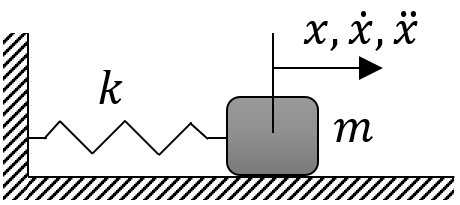
\includegraphics[width=.45\linewidth,trim={0.000bp 0.000bp 0.000bp 3.000bp},clip]{graphics/tomeg_rugo_modell.png}
	\caption{Periodikus mozgást végző tömeg-rugó rendszer}\label{fig:bvp_tomeg_rugo}
\end{figure}

A mozgásegyenlete a fenti rendszernek jól ismert:
\begin{equation}
\ddot{x}= -\frac{k}{m}\,x.
\end{equation}
Mint tudjuk, a rendszer mozgását leíró függvényt az alábbi módon lehet felírni, amennyiben $x_0$ kezdeti kitérítésünk van csak $\tau_0$ időpillanatban kezdeti sebesség nélkül:
\begin{equation}
\varphi(\tau) = x_0\cos\left(\tau\sqrt{k/m}\,T\right) = x_0\cos\left(2\pi\,\tau\right),
\end{equation}
\begin{equation}
\dot{\varphi}(\tau) = -x_0\sqrt{k/m}\sin\left(\tau\sqrt{k/m}\,T\right) = -x_0\sqrt{k/m}\sin\left(2\pi\,\tau\right),
\end{equation}
ahol $T$ a rendszer sajátfrekvenciájának inverze
\begin{equation}
T = 2\pi\sqrt{m/k}.
\end{equation}
A fenti függvényeket a peremérték-megfogalmazáskor kijöttekkel fogjuk összevetni.

A bvp5c megoldóhoz először definiálnunk kell egy időrácsot, amely i\-dő\-pon\-tok\-ban meg kell becsülnünk majd a keresett függvények értékét.
Mivel áttértünk dimenziótlan időre, egy periódus "peremei" a $\tau \in \left \{ 0,1 \right \}$ pontok, valamint megjelent a Cauchy átírásnál $T$ periódusidő, mint ismeretlen paraméter.
\begin{equation}
\begin{bmatrix}
x'(\tau) \\ y'(\tau)
\end{bmatrix} =
T
\begin{bmatrix}
y(\tau) \\  -\frac{k}{m}\,x(\tau)
\end{bmatrix}
\end{equation}
A harmonikus oszcillátor konzervatív: a periodikus pályák amplitúdó szerint családot alkotnak. Ezért az általános periodicitási és fázisfeltétel mellett az amplitúdót is rögzíteni kell. Az $x(0)=x_0$, $x(1)=x_0$, $v(0)=0$ három feltétel használata sem megfelelő: a periódus végén $v(T)=0$, így a véghelyzet periódusidő szerinti deriváltja nulla, és a linearizált peremfeladat szinguláris.

Ebben a szimmetrikus példában egyszerűbb egy \emph{negyed periódust} számítani. Legyen $Q=T/4$ és $\theta=t/Q\in[0,1]$. A megoldandó feladat:
\[
\frac{d}{d\theta}\begin{pmatrix}x\\v\end{pmatrix}
=Q\begin{pmatrix}v\\-(k/m)x\end{pmatrix},\qquad
x(0)=x_0>0,\quad v(0)=0,\quad x(1)=0.
\]
Két differenciálegyenlethez és az egyetlen ismeretlen $Q$ paraméterhez három peremfeltétel tartozik. Az első zérushelyet keressük, $v(1)<0$ mellett, ezért $\partial_Q x(Q)=v(Q)\neq0$. A megfelelő kezdeti becslés az első negyed periódushoz választja ki a megoldást; ezt a kód az $x>0$ belső feltétellel is ellenőrzi. A teljes periódus $T=4Q$. Ez a szimmetriára épülő konstrukció a harmonikus példára vonatkozik, általános határciklusnál a korábban bemutatott periodicitási és fázisfeltételt kell használni.

A függelékben megadott teljes programot \texttt{mass\_spring\_bvp\_v3.m} néven mentsük el, majd a MATLAB aktuális könyvtárából a \lstinline|[T,sol] = mass_spring_bvp_v3;| paranccsal indítsuk. Az alapértékek $k=10$, $m=5$, $x_0=1$; más értékek például a \lstinline|mass_spring_bvp_v3(10,5,1)| hívással adhatók meg. A differenciálegyenletet és a peremfeltételeket leíró függvények ugyanebben a fájlban szerepelnek, külön segédfájl nem szükséges.
\phantomsection\label{use:spring_bvp}A teljes MATLAB-program az A függelék \ref{ap:spring_bvp}. szakaszában található (\pageref{ap:spring_bvp}. oldal).

A kód kiírja a $T=4Q$ eredményt és a $2\pi\sqrt{m/k}$ analitikus periódust, az ábrán pedig összehasonlítja a numerikus és az analitikus megoldást. A kód a négy negyedperiódust a numerikus megoldás tükrözésével és előjelváltásaival állítja össze. A kék görbe az analitikus megoldás, a narancssárga körök a peremfeladatból származó értékek. Az elmozdulás és a sebesség külön panelen látható, saját mértékegységgel. Az ábra 16 cm széles, feliratai 11 pontosak; a PDF-et átméretezés nélkül illesztjük be. A program a vektoros PDF- és SVG-fájlt is elmenti.
A teljes periódusra folytatott pozíciót és sebességet a \ref{fig:bvp_tomeg_rugo_traj_vel}. ábra szemlélteti.

\begin{figure}[ht]
	\centering
	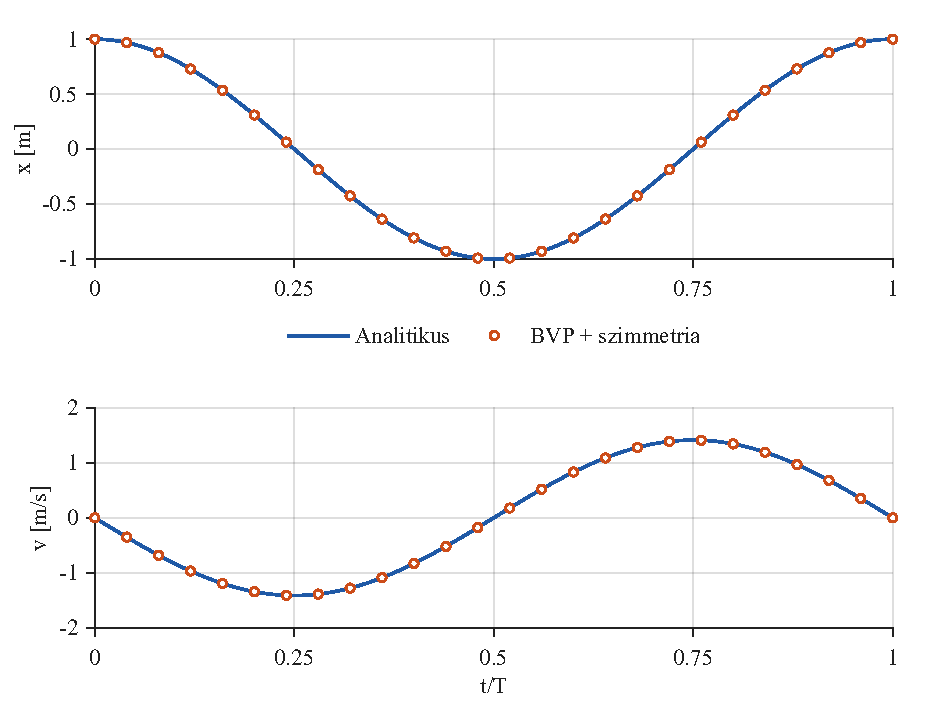
\includegraphics{graphics_v3/mass_spring_bvp.pdf}
	\caption{Tömeg--rugó rendszer teljes periódusa: fent az elmozdulás, lent a sebesség, $k=10$ N/m, $m=5$ kg, $x_0=1$ m mellett. A \texttt{bvp5c} negyedperiódus-megoldását szimmetriával folytatjuk; a körök és az analitikus görbe gyakorlatilag fedik egymást.}\label{fig:bvp_tomeg_rugo_traj_vel}
\end{figure}

\section{A teljes periodikus peremfeladat folytatása}
\label{sec:full_pal}
A $T=T_{\mathrm{BVP}}(\mu)$ grafikon feltevése egyszerű példákban használható, de általános visszahajlásnál a pálya nem egyértékű függvénye $\mu$-nek. Ilyenkor a teljes $y=(z(\cdot),T,\mu)$ megoldás az ismeretlen. Egy autonóm, sima rendszerre a korrekció egyidejűleg oldja meg
\begin{align}
z'(\tau)&=T F(z(\tau),\mu),\qquad z(0)=z(1),\\
0&=\int_0^1\langle z(\tau)-z_i(\tau),z_i'(\tau)\rangle\,d\tau,\\
\Delta s&=\int_0^1\langle z(\tau)-z_i(\tau),v_z(\tau)\rangle_W\,d\tau\notag\\
&\quad+w_T(T-T_i)v_T+w_\mu(\mu-\mu_i)v_\mu.
\end{align}
A második sor fázisfeltétel, a harmadik a pseudo-arclength feltétele; a súlyok és a normalizált érintő ugyanahhoz a skálázáshoz tartoznak. Konzervatív pályacsaládnál további energiarögzítés és szükség esetén megfelelő kibővítés kell, ahogy a harmonikus példánál is láttuk. Több folytonos szegmens esetén a teljes diszkretizált rendszer a szegmenseket, a kapcsolási vagy reset feltételeket és az ismeretlen szegmensidőket is tartalmazza. Ez a felírás nem oszt egy érintőkomponenssel, és egyszerű fordulóponton is használható \cite{auto}.

\section{Pseudo-arclength continuation periodikus pályákra}

Ebben az alfejezetben két egyszerű periodikus pályacsaládot vizsgálunk. Megkülönböztetjük a rögzített paraméterű peremfeladat megoldását, a közvetlen paraméterléptetést és a visszahajláshoz szükséges pseudo-arclength continuation eljárást.
Ehhez ki kell választanunk majd egy bifurkációs paramétert, amely függvényében kíváncsiak vagyunk, hogyan alakul a periodikus mozgás.
Az első feladat az előbb vizsgált tömeg-rugó rendszer paraméterfüggését mutatja be; a másodikban a merevség a kitérés előjelével vált, ezért két folytonos szegmenst illesztünk össze.

\subsection{Példa 1: tömeg-rugó rendszer}
\examplebody


A pseudo-arclength continuation eljárás használatához ki kell választanunk egy bi\-fur\-ká\-ci\-ós paramétert, amit jelöljön $\mu$.
A példa során először vizsgáljuk a rugómerevség $(\mu = k)$, később a tömeg $(\mu =m)$ hatását (ilyenkor a többi paraméter konstans).
A \eqref{eq:pszeudo_ivhossz_alapegyenlet} egyenlet alakja paraméterkövetés során az alábbi formájú:
\begin{equation}
\begin{cases}
0 = \left< \mathbf{x}_{i+1} - \mathbf{x}_i, \mathbf{v}_i \right> - \Delta s \\
0 = T_{i+1} - T_{\mathrm{BVP}}(\mu_{i+1}),
\end{cases}
\label{eq:pszeudo_per_kov}
\end{equation}
\begin{equation}
\mathbf{x_i}= \begin{bmatrix}
\mu_{i} & T_{i}
\end{bmatrix}^\mathrm{T},
\end{equation}
ahol $T_{\mathrm{BVP}}(\mu_{i+1})$ a peremfeladat-megoldó által számolt periódusidő. Ez a csökkentett felírás itt megengedett, mert $k,m>0$ mellett $T=2\pi\sqrt{m/k}$ sima, egyértékű grafikon. Általános pályacsaládra a \ref{sec:full_pal}. szakasz teljes feladatát kell használni.
A pseudo-arclength continuation eljárást a \ref{sec:pseudo_ivhossz} alfejezetben bemutatott módon kell alkalmazni, és a benne található $T_{\mathrm{BVP}}(\mu_{i+1})$ értékét a \ref{sec:per_palya_perem_megfog} alfejezetben leírt módon kell meghatározni a \eqref{eq:pszeudo_per_kov} egyenletrendszer megoldása közben.
A kapott eredményeket összevetettük az analitikusan kiszámítottakkal, és látható, hogy a pályakövetés illeszkedik az analitikusan előállított görbékre, ld. \ref{fig:pszeudo_tomeg_rugo_k}. és \ref{fig:pszeudo_tomeg_rugo_m}. ábrák.

A fájl neve: \texttt{spring\_continuation\_v3.m}. Indítás MATLAB-ban: \lstinline|spring_continuation_v3|. Minden periódust a \texttt{bvp5c} számít, az analitikus képlet csak a kezdeti becsléshez és az eredmény ellenőrzéséhez szerepel. A szelőirányú prediktort kétdimenziós Newton-korrektor követi: a periódus maradéka mellett a prediktorra merőleges hipersík feltételét oldjuk meg. A periódus paraméterderiváltját középpontos differenciával becsüljük. A korrektor így nem igényel \texttt{fsolve}-ot vagy külön segédfájlt.

A merevségkövetés $k=2$ N/m-ről indul, $m=5$ kg és $\Delta s=0{,}5$ mellett; a tömegkövetés $m=1$ kg-ról indul, $k=10$ N/m és $\Delta s=1$ mellett. Mindkét esetben két kezdőpont után 30 korrekciós lépést végzünk. A lépéshosszt itt a megadott egységekben felírt $(\mu,T)$ koordináták euklideszi normájával mérjük; más egységek vagy léptékek esetén skálázás szükséges. Az analitikus görbe és a numerikus körjelölők egyezése a peremfeladatot és a követést ellenőrzi; ezen a monoton ágon nincs visszahajlás.
\phantomsection\label{use:spring_cont}A teljes MATLAB-program az A függelék \ref{ap:spring_cont}. szakaszában található (\pageref{ap:spring_cont}. oldal).

\begin{figure}[!htbp]
	\centering
	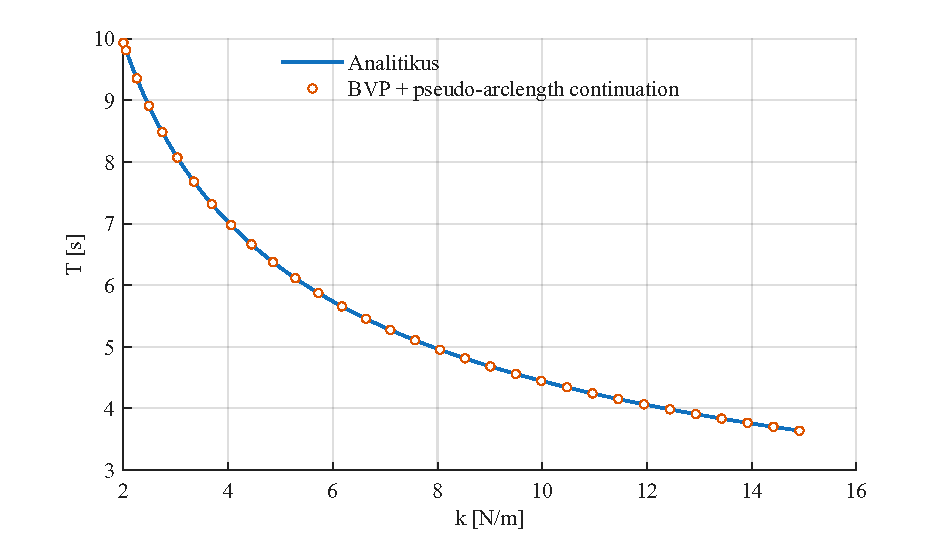
\includegraphics{graphics_v3/spring_k.pdf}
	\caption{Periodikus pályák követése $k$ paraméter függvényében, $\Delta s = 0.5$}\label{fig:pszeudo_tomeg_rugo_k}
\end{figure}

\begin{figure}[!htbp]
	\centering
	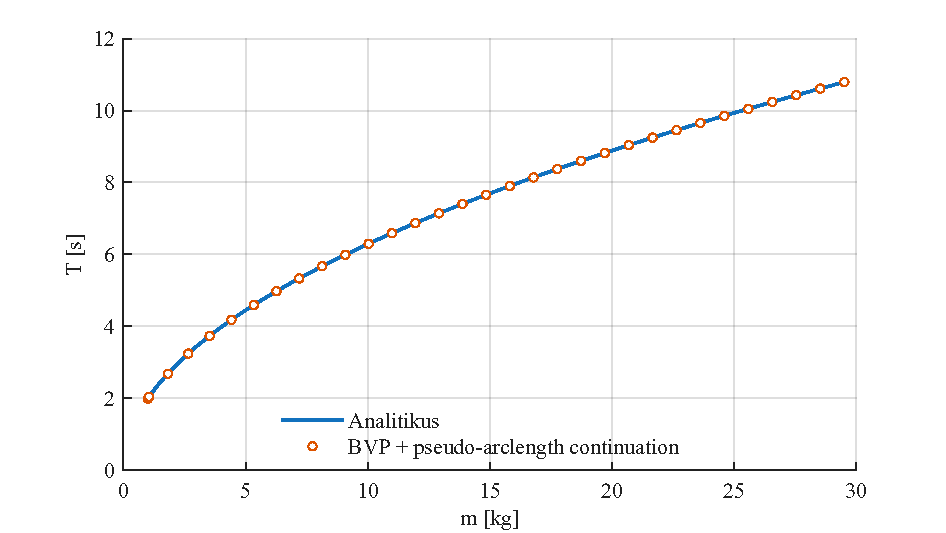
\includegraphics{graphics_v3/spring_m.pdf}
	\caption{Periodikus pályák követése $m$ paraméter függvényében, $\Delta s = 1$}\label{fig:pszeudo_tomeg_rugo_m}
\end{figure}

\FloatBarrier
\exampleend

\subsection{Példa 2: kétféle merevségű rugó}
\examplebody

A több szegmensből összeállított peremfeladatot egy egységnyi tömegű, kétféle rugómerevségű oszcillátoron mutatjuk be:
\begin{equation}\label{eq:bilinear_oscillator}
\ddot x=\begin{cases}-k_+x,&x>0,\\-k_-x,&x<0,\end{cases}
\qquad k_+,k_->0.
\end{equation}
A kapcsolófelület $x=0$. Az állapot folytonos, nincs sebességugrás. A vektormező itt folytonos, csak a deriváltja vált: ez a piecewise-smooth rendszerek legegyszerűbb esete. A kapcsolófelületen a saltation-mátrix az identitás, ezért ez a példa a szegmensek illesztését tanítja; a nemtriviális ütközési korrekciót az ütköző oszcillátor mutatja be.

Induljunk $x(0)=0$, $v(0)=V>0$ állapotból. A pozitív és negatív félhullámot külön $[0,1]$ időskálára írjuk át, ismeretlen $T_+$ és $T_-$ időkkel. A négy komponens $(x_+,v_+,x_-,v_-)$, a hat peremfeltétel pedig
\begin{align}
x_+(0)&=0,&v_+(0)&=V,&x_+(1)&=0,\\
x_-(0)&=x_+(1),&v_-(0)&=v_+(1),&x_-(1)&=0.
\end{align}
Az első feltétel a fázist, a második az energiaszintet rögzíti. A végső sebesség $v_-(1)=V$ az energiamegmaradásból és az első félhullámok kiválasztásából következik; külön előírva túlhatároznánk ezt a hatfeltételes feladatot. Az analitikus ellenőrzés:
\begin{equation}
T_+=\frac{\pi}{\sqrt{k_+}},\qquad
T_-=\frac{\pi}{\sqrt{k_-}},\qquad T=T_++T_-.
\end{equation}
A $k_+=4$, $k_-=1$, $V=1$ választásnál $T=3\pi/2$. A kód négy állapotot és két ismeretlen időt kezel, és megköveteli a megfelelő félhullámok előjelét. Az analitikus alak csak kezdeti becslés és ellenőrzés; az időtartamokat a peremfeladat-megoldó számítja.
A teljes, önálló programot \texttt{bilinear\_bvp\_v3.m} néven mentve a \lstinline|[T,sol] = bilinear_bvp_v3;| paranccsal indíthatjuk. A két lokális függvény ugyanebben a fájlban szerepel. A program a félhullámok illesztésén túl a teljes periódust ábrázolja, és vektoros PDF- és SVG-fájlt ment. A feliratok 11 pontosak; az ábrát átméretezés nélkül illesztjük be.
\phantomsection\label{use:bilinear}A teljes MATLAB-program az A függelék \ref{ap:bilinear}. szakaszában található (\pageref{ap:bilinear}. oldal).

\begin{figure}[htbp]
\centering
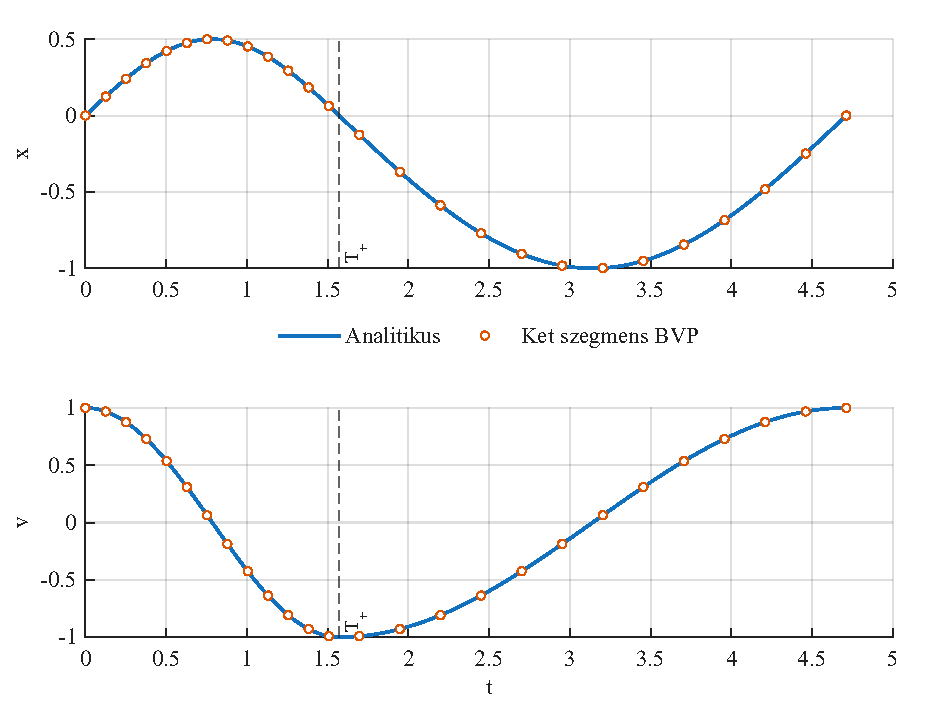
\includegraphics{graphics_v3/bilinear_bvp.pdf}
\caption{A kétféle merevségű oszcillátor egy teljes periódusa, $k_+=4$, $k_-=1$, $V=1$ mellett. Fent az elmozdulás, lent a sebesség; folytonos vonal: analitikus megoldás, körök: a két szegmensből illesztett BVP-megoldás. A szaggatott vonal $T_+=\pi/2$ időpontját jelöli.}\label{fig:bilinear_bvp}
\end{figure}

A \ref{fig:bilinear_bvp}. ábrán a merevebb, pozitív oldali félhullám rövidebb ($T_+=\pi/2$), és kisebb a kitérése ($x_{\max}=1/2$). A lágyabb, negatív oldalon $T_-=\pi$ és $x_{\min}=-1$. Az illesztéskor $x=0$ és $v=-1$ mindkét szegmensben ugyanaz: nincs állapotugrás. A periódus végén $(x,v)=(0,1)$, tehát a pálya záródik. A pontok és az analitikus görbék egyezése külön-külön ellenőrzi a két szegmenst és az illesztésüket.


Ez rögzített paraméterű többfázisú BVP, önmagában nem pseudo-arclength continuation. Itt $k_+$ szerinti közvetlen paraméterléptetés is elegendő: $T(k_+)=\pi/\sqrt{k_+}+\pi/\sqrt{k_-}$ nem hajlik vissza. Általános visszahajlásnál a \ref{sec:full_pal}. szakasz teljes kibővített rendszerét kell használni. A korábbi, összetettebb SLIP-peremfeladat kódja további alkalmazásként a \texttt{codes/slip\_bvp\_v3.m} fájlban elérhető; nem szükséges a két szegmens illesztésének megértéséhez.
\exampleend

\section{Stabilitási és grazing-határok követése}
Egy bifurkációs görbe követéséhez két \emph{fizikai} paramétert választunk, például az ütköző oszcillátor gerjesztési frekvenciáját és falhelyzetét, $(\mu_1,\mu_2)=(\omega,\sigma)$. A teljes periodikus peremfeladatot egy skalár kritikus feltétellel, majd a pseudo-arclength egyenlettel egészítjük ki. A $\lambda$ multiplikátor nem új, szabad fizikai paraméter: a pálya monodrómia-mátrixából kell számítani vagy sajátvektor-egyenlettel csatolni.

Példák: nemtriviális $\lambda=+1$ ciklusok saddle-node bifurcation eseményének jelöltje, $\lambda=-1$ period-doubling bifurcation jelöltje, nemvalós $|\lambda|=1$ pár Neimark--Sacker-bifurkáció jelöltje. Az autonóm időeltolás és a konzervált energia triviális egységnyi multiplikátorait előbb ki kell szűrni, például megfelelő Poincaré-metszettel és energiaszintre megszorítással. A kritikus feltétel önmagában nem garantál nemelfajult bifurkációt.

Grazing-határnál az eseménypont a kapcsolófelületen van és $H_xF=0$; a reguláris esethez $a_H\neq0$ is kell. A transzverzális saltation-mátrixot a grazing-pontban nem szabad véges numerikus értékként használni.

\chapter{Eseménykezelés, súrlódás és modellválasztás}\label{sec:practical}
Az előző fejezetek megadták a kapcsolófelületen érvényes dinamikát, a perturbációk korrekcióját és a periodikus pályák számítását. A gyakorlatban ezekhez még egy döntés társul: milyen eseménynél melyik mozgásegyenletre térünk át? Ebben a fejezetben néhány egyszerű modellen követjük végig a szabad mozgást, az ütközést, a tapadást és a közelítő sima leírást. A példákban az esemény, a numerikus módszer és a fizikai modell szerepét külön kezeljük.

\section{Eseményvezérelt numerikus integrálás}\label{sec:event_numerics}
A numerikus eseménykezelés és az időléptetés megkülönböztetésének könyvbeli háttere: \cite[2.6.1. szakasz]{dib}.

\subsection{Miért nem elegendő egy előjelfüggvény?}
Egy sima szakaszon az integrátor a megadott vektormezőt követi. A kapcsolás időpontját a $H(x(t),t)=0$ eseményegyenlet adja. Ha egyetlen differenciálegyenlet jobb oldalába tesszük a kapcsolást, például egy \texttt{sign} függvénnyel, a megoldó egy lépésen belül különböző dinamikákat mintavételezhet. Így az eseményidő és az ütközési sebesség hibája akkor is jelentős lehet, ha az állapotgörbe szemre sima.

Az eseményvezérelt eljárás egy sima szakaszt az első releváns eseményig integrál, az eseményállapotból alkalmazza az előírt $x^+=R(x^-)$ reset leképezést vagy módváltást, majd innen indul újra. A variációs mátrixot külön is át kell képezni a megfelelő saltation-mátrixszal; az állapot reset leképezésa ezt nem végzi el automatikusan. Több eseményfelület esetén mindegyikhez meg kell adni az irányt és az átmeneti szabályt. Egyidejű kontaktusoknál az egymás utáni önkényes reset leképezés sorrendfüggő eredményt adhat: ilyenkor közös kontaktusmodell szükséges.

\subsection{Pattogó labda: az esemény és az újraindítás}
\examplebody

Egy $h_0$ magasságból elengedett labdára, légellenállás nélkül,
\begin{equation}\label{eq:ball_flow}
\dot h=v,\qquad \dot v=-g,\qquad h>0.
\end{equation}
A talaj elérése $H(h,v)=h=0$, de csak $v^-<0$ esetén ütközés. A reset leképezés
\begin{equation}\label{eq:ball_reset}
h^+=0,\qquad v^+=-rv^-,\qquad 0<r<1.
\end{equation}
A helyzet folytonos; a sebesség ugrik. A MATLAB-eseményfüggvény három kimenete itt: \texttt{value=h}, \texttt{isterminal=1}, \texttt{direction=-1}. A lefelé történő átlépés kiválasztása megkülönbözteti a becsapódást az ütközés utáni felfelé indulástól. Az integrálást a visszaadott eseményidőnél és eseményállapotnál indítjuk újra \cite{matlab_events}.

A függelékben közölt program nyolc becsapódást számít. A lépéskorlát a várható repülési időhöz igazodik. Az újraindulás pillanatában a felfelé mozgó állapot eseményértékét kicsiny pozitív számra állítjuk; ez csak a már kezelt kezdőgyök ismételt észlelését kerüli el, a fizikai helyzetet nem tolja el. Az ütközés előtti és utáni állapotot azonos időbélyeggel tároljuk, hogy a sebességugrás megmaradjon.
\phantomsection\label{use:ball}A teljes MATLAB-program az A függelék \ref{ap:ball}. szakaszában található (\pageref{ap:ball}. oldal).
\exampleend

\subsection{Eseményhiba, kihagyott gyök és konvergencia}
Transzverzális eseménynél legyen $\dot H=H_xF+H_t\neq0$. Egy kicsiny $\delta H$ eseményfüggvény-hiba elsőrendű időhibája
\begin{equation}\label{eq:event_time_error}
\delta t\simeq-\frac{\delta H}{H_xF+H_t}.
\end{equation}
Ezért a grazinghez közeledve ugyanaz a távolsághiba egyre nagyobb időhibát okozhat. Pontos grazing esetén a nevező nulla, a lineáris hibabecslés nem használható; a 4. fejezet négyzetgyökös időskálája lép a helyére.

Az eseménykeresés előjelváltásra épül, ezért két lépésvégpont között páros számú metszés, illetve érintőleges gyök észrevétlen maradhat. A \texttt{MaxStep} és a toleranciák csökkentése segíthet, de az érintés felismerését önmagában nem garantálja. A sűrűbb kimeneti időrács nem azonos a belső lépésköz korlátozásával. A MATLAB dokumentációja külön jelzi az első integrálási lépés terminális eseményeinek korlátozását is; rövid repülési szakasznál ezért az első lépést is korlátozzuk \cite{matlab_events}.

A gyakorlati ellenőrzés tárgya ne csak a pályarajz legyen: kisebb toleranciával és felezett maximális lépéssel hasonlítsuk össze az eseményidőket, a becsapódási sebességeket és az események sorrendjét. Eltérő eseményszámnál előbb a pálya típusát kell tisztázni, és csak utána a monodrómia sajátértékeit összevetni. A labdánál az első ütközés pontos ideje $t_1=\sqrt{2h_0/g}$, sebessége $v_1^-=-\sqrt{2gh_0}$: ezek egyszerű referenciaértékek.

\section{Stick--slip Coulomb-súrlódással}\label{sec:stick_slip}
\subsection{Rugós tömeg mozgó szalagon}
\examplebody

A szalagon mozgó súrlódásos oszcillátor könyvbeli motivációja a \cite[1.3.2. szakasz]{dib}; itt ennek egyszerűbb, gerjesztés nélküli, két súrlódási szinttel leírt tanpéldáját használjuk.

\begin{figure}[htbp]
\centering
% Mechanical schematic; fixed 11 pt labels, no document scaling.
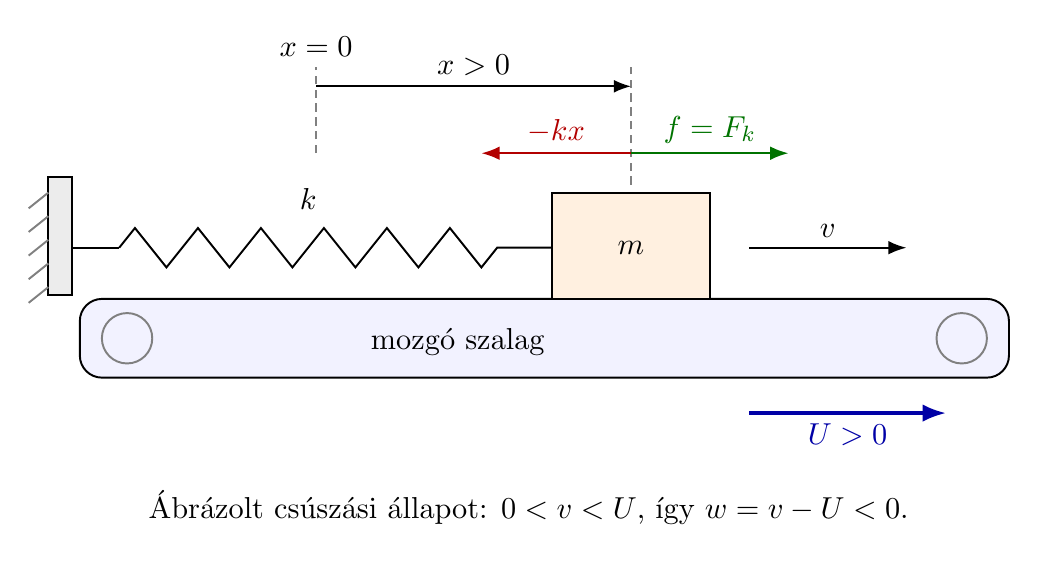
\begin{tikzpicture}[x=1cm,y=1cm,>=Latex,line width=.7pt,
 font=\normalfont\fontsize{11}{13.2}\selectfont]
\draw[fill=gray!15] (1.1,1.7) rectangle (1.4,3.2);
\foreach \y in {1.8,2.1,2.4,2.7,3.0}
  \draw[gray] (1.1,\y)--(.85,\y-.2);
\draw[fill=blue!5,rounded corners=8pt] (1.5,.65) rectangle (13.3,1.65);
\draw[gray] (2.1,1.15) circle (.32);
\draw[gray] (12.7,1.15) circle (.32);
\node at (6.3,1.1) {mozgó szalag};
\draw[->,blue!65!black,very thick] (10,.2)--(12.5,.2)
 node[midway,below] {$U>0$};
\draw (1.4,2.3)--(2,2.3);
\draw (2,2.3)--(2.2,2.55)--(2.6,2.05)--(3,2.55)--(3.4,2.05)
 --(3.8,2.55)--(4.2,2.05)--(4.6,2.55)--(5,2.05)--(5.4,2.55)
 --(5.8,2.05)--(6.2,2.55)--(6.6,2.05)--(6.8,2.3)--(7.5,2.3);
\node[above] at (4.4,2.65) {$k$};
\draw[fill=orange!12] (7.5,1.65) rectangle (9.5,3);
\node at (8.5,2.3) {$m$};
\draw[densely dashed,gray] (4.5,3.5)--(4.5,4.6);
\draw[densely dashed,gray] (8.5,3.1)--(8.5,4.6);
\draw[->] (4.5,4.35)--(8.5,4.35) node[midway,above] {$x>0$};
\node[above] at (4.5,4.6) {$x=0$};
\draw[->,red!70!black,thick] (8.5,3.5)--(6.6,3.5)
 node[midway,above] {$-kx$};
\draw[->,green!45!black,thick] (8.5,3.5)--(10.5,3.5)
 node[midway,above] {$f=F_k$};
\draw[->,thick] (10,2.3)--(12,2.3) node[midway,above] {$v$};
\node[below] at (7.2,-.65) {Ábrázolt csúszási állapot: $0<v<U$, így $w=v-U<0$.};
\end{tikzpicture}

\caption{Rugós tömeg egy jobbra haladó szalagon. A vázlat $x>0$ és $0<v<U$ pillanatnyi állapotot mutat: a rugó balra húz, a kinetikus súrlódás jobbra hat. Az $x=0$ jel a tömeg rugóerő-mentes referenciahelyzetét jelöli; a nyilak hossza nem az erők vagy sebességek aránya.}\label{fig:belt_model}
\end{figure}

A \ref{fig:belt_model}. ábrán a rugó bal vége a laboratóriumhoz rögzített, a szalag viszont $U$ sebességgel mozog. A súrlódás irányát a test és a szalag \emph{relatív} sebessége határozza meg: a bemutatott $v<U$ esetben a szalag jobbra húzza a testet; $v>U$ esetén a súrlódás balra mutatna. Tapadáskor $v=U$, a súrlódás pedig a rugóerő kiegyenlítéséhez igazodik, amíg $|kx|\leq F_s$. A tapadó test tehát a laboratóriumban tovább mozog, miközben a szalaghoz képest áll. Az ábrán csak a vízszintes mozgást meghatározó erőket tüntettük fel.

Legyen $x$ a tömeg rugónyúlása, $v=\dot x$ a laboratóriumi sebessége, a szalag sebessége pedig az állandó $U>0$. A relatív sebesség $w=v-U$. A rugóerő $-kx$, a súrlódási erő $f$. Mechanikai csúszáskor
\begin{equation}\label{eq:coulomb_slip}
m\dot v=-kx-F_k\operatorname{sign}(v-U),\qquad \dot x=v,
\end{equation}
ahol $F_k>0$ a kinetikus súrlódási erő nagysága. Tapadáskor a test együtt halad a szalaggal: $v=U$, $\dot v=0$. Ehhez $f=kx$ szükséges, amely csak
\begin{equation}\label{eq:stick_condition}
|kx|\leq F_s
\end{equation}
esetén lehetséges; $F_s\geq F_k$ a statikus súrlódás határa. A tapadás nem azt jelenti, hogy a test nyugalomban van: ekkor $\dot x=U$.

A felület $H=v-U=0$. Ha $F_s=F_k=F$, a két csúszó mező normális komponense
\[
\ell_+=\frac{-kx-F}{m},\qquad
\ell_-=\frac{-kx+F}{m}.
\]
Így $|kx|<F$ mellett attracting sliding áll fenn, a redukált mozgás $\dot x=U$, $v=U$. A \emph{Filippov-féle sliding} itt éppen \emph{mechanikai tapadást} jelent: az állapot a kapcsolófelületen mozog, miközben a két érintkező test relatív sebessége nulla.

Az $F_s>F_k$ modell több információt tartalmaz, mint a két kinetikus mező Filippov-konvexifikációja. Külön tapadási módot és elengedési szabályt adunk meg. Csúszásból a $v=U$ elérésekor tapadásra váltunk, ha $|kx|\leq F_s$; egyébként a megfelelő csúszó ágon folytatjuk a mozgást. Tapadásból akkor lépünk ki, amikor a szükséges erő a megengedett intervallumon kívülre lépne. $U>0$ esetén a tapadás végén $x=F_s/k$, utána $w<0$ lesz. A határon a továbbhaladás iránya dönt, nem pusztán az egyenlőség.
\exampleend

\subsection{Egy teljes ciklus elemi függvényekkel}
\examplebody

Válasszuk a dimenziótlan $m=k=1$, $U=0{,}3$, $F_s=0{,}6$, $F_k=0{,}4$ értékeket. A tapadás $x_a=2F_k-F_s=0{,}2$ helyről indul, $v=U$ mellett. A test $x_b=F_s=0{,}6$ helyig együtt mozog a szalaggal:
\begin{equation}
x(t)=x_a+Ut,\quad v(t)=U,\quad
T_s=\frac{x_b-x_a}{U}=\frac43.
\end{equation}
Az elengedéstől mért $s$ idővel, a $v<U$ mechanikai csúszási szakaszon $\ddot x+x=F_k$, tehát
\begin{align}\label{eq:stick_slip_exact}
x(s)&=F_k+(F_s-F_k)\cos s+U\sin s,\\
v(s)&=-(F_s-F_k)\sin s+U\cos s.
\end{align}
A $v(s)=U$ egyenlet első \emph{pozitív} gyöke
\begin{equation}\label{eq:slip_duration}
T_l=2\pi-2\arctan\frac{F_s-F_k}{U}\simeq5{,}10718.
\end{equation}
Ekkor $x(T_l)=x_a$, $v(T_l)=U$, és a test ismét tapad. A teljes ciklus $T_s+T_l\simeq6{,}44051$. A megadott szakasz belsejében valóban $v-U<0$, tehát a választott súrlódási irány végig helyes. A \ref{fig:stick_slip_new}. ábrán a zérus relatív sebességű vízszintes részek a tapadási időintervallumok.

\begin{figure}[!htbp]\centering
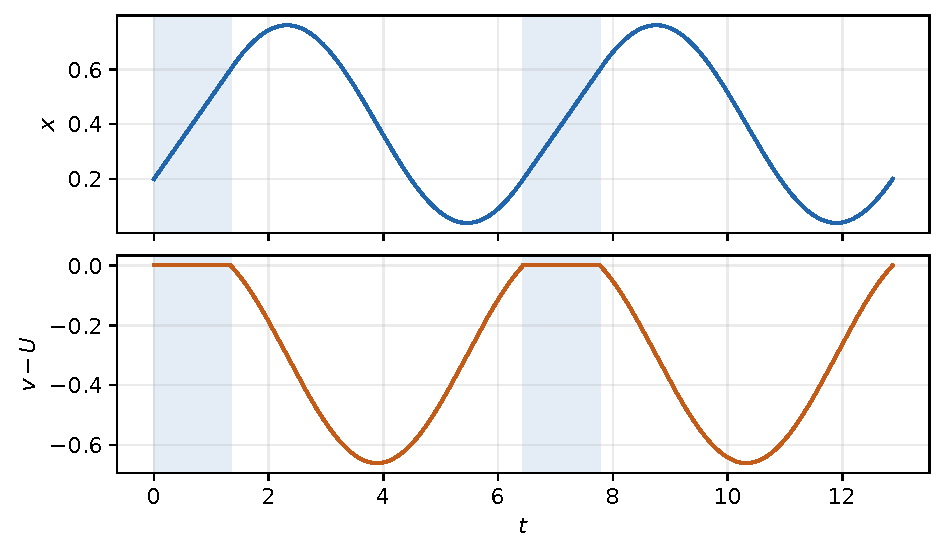
\includegraphics[width=\linewidth]{graphics_v3/stick_slip_cycle.pdf}
\caption{Tapadás és csúszás két egymást követő ciklusban. A kék háttér tapadást jelöl. A laboratóriumi helyzet ekkor változik, a relatív sebesség nulla.}\label{fig:stick_slip_new}
\end{figure}

A kód az egzakt szakaszokat illeszti, így külön ODE-megoldó nélkül ellenőrizhető a váltási logika. Általános gerjesztésnél ugyanezeket a módokat eseményvezérelt integrálással kell összekapcsolni.
\phantomsection\label{use:stick}A teljes MATLAB-program az A függelék \ref{ap:stick}. szakaszában található (\pageref{ap:stick}. oldal).
\exampleend

\section{Zeno-jelenség és tartós kontaktus}\label{sec:zeno}
\subsection{Végtelen sok ütközés véges idő alatt}
A pattogó labda alapmodelljéhez az \cite[1.2. szakasz]{dib}, az ütközések felhalmozódásához és a tapadás kialakulásához a kötet 6.4.3. szakasza ad további hátteret.

Térjünk vissza a labdához. Jelölje $V=\sqrt{2gh_0}$ az első becsapódási sebesség nagyságát, $t_1=V/g$ az első ütközés idejét. Az $n$-edik visszapattanás utáni sebesség $r^nV$, a következő repülés időtartama
\begin{equation}\label{eq:zeno_intervals}
\Delta t_n=\frac{2r^nV}{g},\qquad n=1,2,\ldots.
\end{equation}
Mivel $0<r<1$, a geometriai sor összegezhető:
\begin{equation}\label{eq:zeno_time}
T_Z=t_1+\sum_{n=1}^{\infty}\Delta t_n
=\frac{V}{g}\frac{1+r}{1-r}.
\end{equation}
A $h_0=1\,\mathrm m$, $g=9{,}81\,\mathrm{m/s^2}$, $r=0{,}7$ esetben $T_Z\simeq2{,}55863\,\mathrm s$. Végtelen sok diszkrét esemény történik véges fizikai idő alatt: ez a Zeno-jelenség. A repülési szakaszok száma korlátlanul nő, miközben az állapot $(h,v)=(0,0)$-hoz tart. Ez a modell tulajdonsága, nem integrátorhiba \cite{or_teel}.

\begin{figure}[!htbp]\centering
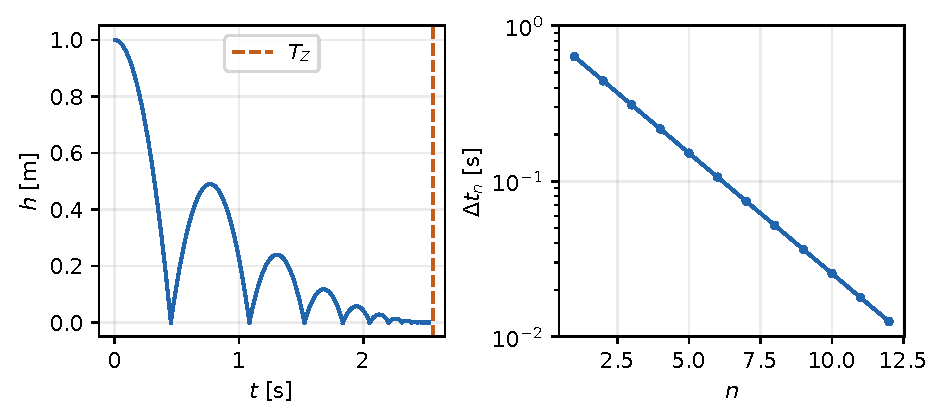
\includegraphics[width=\linewidth]{graphics_v3/zeno_ball.pdf}
\caption{A labda egzakt repülési szakaszai és az ütközési időközök. A jobb oldali logaritmikus skálán a geometriai csökkenés egyenes. Az ábra véges számú szakaszt jelenít meg.}\label{fig:zeno_new}
\end{figure}

A numerikus eseménypattogás ettől eltér: hibás újraindítás vagy kerekítési hiba ugyanazt a gyököt újra és újra megtalálhatja, lényeges időelőrehaladás nélkül. Zeno esetén a pontos repülési időközök is csökkennek. A programunk nyolc ütközés után megáll; nem állítja, hogy addigra a labda fizikailag nyugalomba került.

\subsection{Hogyan folytatjuk a mozgást?}
A szabad esés és a sebesség-reset leképezés önmagában nem ad kontaktuserőt. $T_Z$ után a nyugalomban maradáshoz új módot vezetünk be:
\begin{equation}
h=0,\quad v=0,\quad N=mg,\quad \dot h=\dot v=0,
\end{equation}
ahol $N\geq0$ a talaj nyomóereje. A merev, egyoldali kontaktus feltételei
\begin{equation}\label{eq:contact_complementarity}
h\geq0,\qquad N\geq0,\qquad hN=0.
\end{equation}
Szabad repülésben $N=0$; tartós kontaktusban a kényszert fenntartó erőt számítjuk. Ezek önmagukban nem helyettesítik a becsapódás impulzustörvényét. Általános külső erőnél a kontaktus csak addig tartható fenn, amíg nem igényelne húzó talajerőt; ellenkező esetben elválás történik. A Zeno-idő utáni folytatás tehát kifejezett modellkiegészítés \cite{goebel_sanfelice}.

Ha kis sebességnél numerikusan nyugalomra váltunk, ennek pontossága is becsülhető. Az aktuális visszapattanás utáni $u>0$ sebességtől a még hátralévő repülési idő
\[
T_{\mathrm{marad}}=\frac{2u}{g(1-r)},\qquad
h_{\mathrm{kov}}=\frac{u^2}{2g}.
\]
Egy $u<v_{\mathrm{tol}}$ leállítás legfeljebb $v_{\mathrm{tol}}^2/(2g)$ következő emelkedést hagy el, de a hátralévő idő $r\to1$ esetén nagy lehet. A sebességküszöböt ezért fizikai magasság- és időpontossághoz kell kötni; nem általános gyógyír minden sűrű eseménysorozatra.

\section{Discontinuity-induced bifurcations}\label{sec:boundary_bifs}
A sima bifurkációknál a pálya ugyanazon sima dinamikán belül veszti el stabilitását vagy létezését. Szakaszos rendszernél az is változást okozhat, hogy a pálya eléri a kapcsolási határt. A három itt megkülönböztetett helyzet: egy diszkrét leképezés fixpontjának border-collision bifurcation eseménye, egy folytonos pálya grazing eseménye és egy Filippov sliding szakasz megjelenése. A határ elérése önmagában még nem mondja meg az új pálya stabilitását \cite{champneys_dib}.

\subsection{Border-collision bifurcation egy kétszakaszos leképezésben}
\examplebody

A következő elemi példa a \cite[1.4.3. és 3.4. szakasz]{dib} által tárgyalt folytonos, szakaszonként lineáris leképezések körébe tartozik.

Tekintsük a folytonos, de a határon nem differenciálható modellt:
\begin{equation}\label{eq:border_map}
x_{n+1}=P(x_n;\mu)=
\begin{cases}\mu+\frac12x_n,&x_n\leq0,\\
\mu-\frac32x_n,&x_n>0.
\end{cases}
\end{equation}
$\mu<0$ mellett $x_*=2\mu<0$ stabil fixpont, multiplikátora $1/2$. $\mu=0$-nál eléri a $x=0$ határt. $\mu>0$ mellett a jobb ág fixpontja $x_*=2\mu/5>0$, multiplikátora $-3/2$, tehát instabil. A kétoldali derivált a kritikus pontban nem létezik; nem történt egy sima multiplikátor folyamatos áthaladása a $-1$ értéken.

Keressünk a pozitív paraméteroldalon kétciklust, $x_L<0<x_R$ pontokkal. A két feltétel
\[
x_R=\mu+\tfrac12 x_L,\qquad
x_L=\mu-\tfrac32 x_R
\]
megoldása
\begin{equation}\label{eq:border_two_cycle}
x_L=-\frac{2\mu}{7},\qquad x_R=\frac{6\mu}{7}.
\end{equation}
Az ágfeltételek $\mu>0$ esetén teljesülnek, a kétlépéses multiplikátor $(1/2)(-3/2)=-3/4$, így a ciklus lokálisan aszimptotikusan stabil. A stabil fixpontot a border-collision bifurcation után stabil kétciklus váltja fel. A \ref{fig:border_new}. ábra az egzakt ágakat mutatja; a rövid kód tranziens utáni iterációkkal állítja elő a stabil ágakat. Instabil ágat egyszerű előreiterálással általában nem kapunk meg.

\begin{figure}[!htbp]\centering
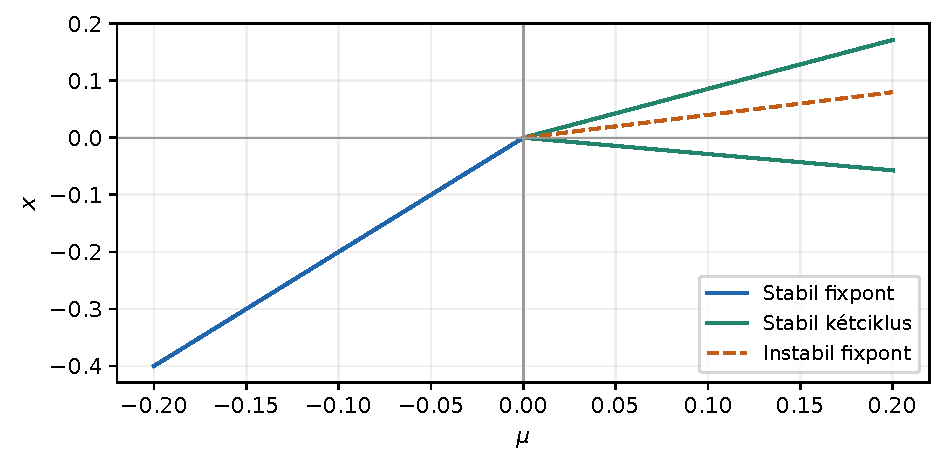
\includegraphics[width=\linewidth]{graphics_v3/border_collision.pdf}
\caption{Border-collision bifurcation $\mu=0$-nál. Folytonos vonal: stabil fixpont, illetve a stabil kétciklus két pontja. Szaggatott vonal: instabil fixpont.}\label{fig:border_new}
\end{figure}
\phantomsection\label{use:border}A teljes MATLAB-program az A függelék \ref{ap:border}. szakaszában található (\pageref{ap:border}. oldal).
\exampleend

\subsection{Grazing és sliding szakasz születése}
\examplebody

A sliding bifurcations osztályozását és a grazing--sliding eset levezetését lásd \cite[8.1. és 8.3.2. szakasz]{dib}.

A 4. fejezet ütköző oszcillátoránál a grazing feltétele $H=0$, $H_xF=0$, $a_H>0$. Ekkor a simán továbbvezetett pálya a kontaktus határát érinti, és a visszatérési leképezésben négyzetgyökös korrekció jelenhet meg. Ez nem azonos a \eqref{eq:border_map} véges meredekségű, szakaszonként lineáris modelljével.

Filippov-rendszerben más mechanizmust látunk. Lokális, dimenziótlan példaként legyen $H=y$, és
\begin{equation}\label{eq:local_sliding_birth}
F_+(x,y)=\begin{pmatrix}1\\x\end{pmatrix}\ (y>0),\qquad
F_-(x,y)=\begin{pmatrix}1\\1\end{pmatrix}\ (y<0).
\end{equation}
A $y=0$, $x<0$ félegyenesen a két mező a felületre mutat, ezért $\dot x=1$, $\dot y=0$ sliding mozgás adódik. A felső sima pályák $dy/dx=x$ alapján
\[
y=\tfrac12x^2+c
\]
parabolák. $c>0$ mellett nincs kontaktus, $c=0$ esetén érintés történik az origóban. $c<0$ esetén a beérkező pálya $x=-\sqrt{-2c}$ pontban eléri a felületet, sliding mozgással jut rajta az origóig, majd elhagyja azt a felső tartomány felé. A sliding szakasz időtartama $\sqrt{-2c}$. Ezzel közvetlenül látható egy sliding szakasz születése.

Itt $c$ a beérkező pályát jelöli, nem a vektormező paramétere. Egy teljes rendszerben a globális visszatérés és egy fizikai paraméter határozhatja meg $c$ értékét. A lokális példa ezért a grazing--sliding mechanizmusát szemlélteti; önmagában nem bizonyít periodikus pályán bekövetkező bifurkációt. A sliding szakasz az ide érkező pályák egy részét ugyanahhoz a kilépő állapothoz vezeti, így a visszatérési leképezés információt veszíthet és nem feltétlenül invertálható \cite{champneys_dib}.

\begin{figure}[!htbp]\centering
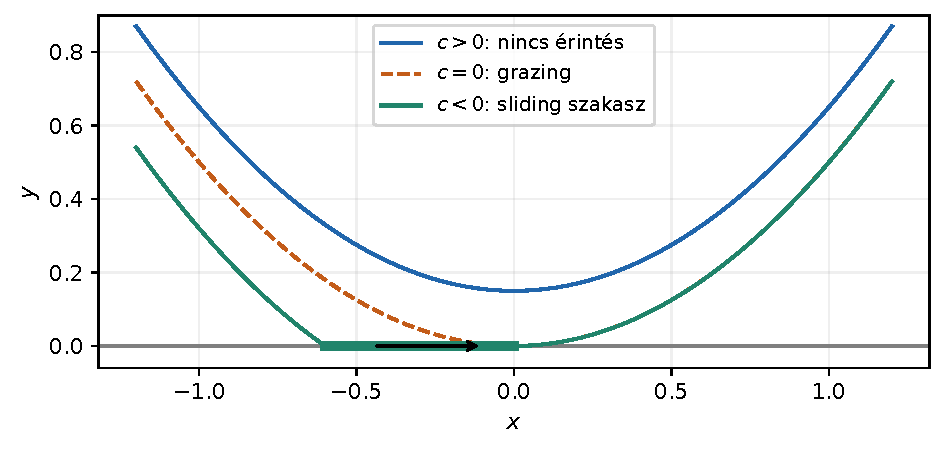
\includegraphics[width=\linewidth]{graphics_v3/sliding_birth.pdf}
\caption{Sliding szakasz megjelenése a lokális példában. A zöld pálya a kapcsolófelületen az origóig halad, majd a felső tartományba lép. A mozgás mindenütt növekvő $x$ irányú.}\label{fig:sliding_birth_new}
\end{figure}
\exampleend

\section{Regularizáció: mikor segít a simítás?}\label{sec:regularization}
\subsection{A simított modell felírása}
Az ideális kapcsolást gyakran folytonos átmenettel helyettesítjük. Egy $H=0$ felület körül például
\begin{equation}
F_\varepsilon=\frac{1+\phi(H/\varepsilon)}2F_+
+\frac{1-\phi(H/\varepsilon)}2F_-,\qquad \phi(s)=\tanh s
\end{equation}
ad sima vektormezőt, ha a két oldali mező is sima a szükséges környezetben. $\varepsilon>0$ az átmenet szélessége, mértékegysége $H$-éval azonos. A regularizáció kapcsolatot teremt a sima és a Filippov-leírás között, de a megoldások és bifurkációk egyezése további feltételeket igényel \cite{sotomayor_teixeira}.

\subsection{Amikor segít: egy csúszó test lefékeződése}
\examplebody

Legyen a tömeg és a Coulomb-súrlódási erő dimenziótlanul egy, külső erő ne hasson, a kezdeti sebesség pedig $v(0)=1$. A test mozgás közben állandóan lassul, megállás után pedig nyugalomban marad. Az ideális Filippov-modell és megoldása:
\[
\dot v\in-\operatorname{Sign}(v),\qquad
v(t)=\max(1-t,0),\quad t\geq0,
\]
ahol $\operatorname{Sign}(v)=\{\operatorname{sign}(v)\}$, ha $v\neq0$, és $\operatorname{Sign}(0)=[-1,1]$. A megállás időpontja $t=1$.

A simítás ugyanennek az egyszerű modellnek a jobb oldalát teszi folytonossá:
\[
\dot v_\varepsilon=-\tanh(v_\varepsilon/\varepsilon),\qquad
v_\varepsilon(0)=1.
\]
Így egy szokásos sima ODE-megoldóval, külön megállási esemény és módváltás nélkül számíthatjuk a lassulást. A példát kézzel is ellenőrizhetjük: $z=\sinh(v_\varepsilon/\varepsilon)$ bevezetésével $\dot z=-z/\varepsilon$, tehát
\begin{equation}\label{eq:regularization_braking_exact}
v_\varepsilon(t)=\varepsilon\operatorname{arsinh}
\left[\sinh(1/\varepsilon)e^{-t/\varepsilon}\right].
\end{equation}
A simított sebesség pozitív marad, és monoton nullához tart. Az ideális sebességtől vett eltérés $0\leq t\leq1$ között nő, utána csökken; maximuma ezért $t=1$-nél van:
\[
0\leq v_\varepsilon(t)-\max(1-t,0)
\leq\varepsilon\operatorname{arsinh}\!\left(\frac{1-e^{-2/\varepsilon}}2\right)
<0{,}482\varepsilon.
\]
Például $\varepsilon=0{,}01$ mellett a sebességhiba \emph{minden} $t\geq0$ időpontban kisebb $0{,}00482$-nél, a nyugalmi határállapot pedig helyes. Ha a kérdés a sebesség lefutása adott pontossággal, a regularizáció itt jól használható, és a hiba $\varepsilon$ csökkentésével kontrollálható. A pontos, véges idejű megállást azonban nem őrzi meg: ehhez továbbra is az ideális eseménykezelés szükséges. A kis $\varepsilon$ miatti rövid relaxációs időt a numerikus megoldónak fel kell oldania.

A \ref{fig:regularization_braking}. ábra a numerikus simított megoldásokat az ideális sebességgel hasonlítja össze. Az alsó panel a megállás környéki hibát nagyítja ki: a legnagyobb eltérés $t=1$-nél jelentkezik, és $\varepsilon$ csökkentésével arányosan mérséklődik. A teljes, mindkét példát előállító MATLAB-kód az A függelék \ref{ap:regularization}. szakaszában található.
\begin{figure}[htbp]\centering
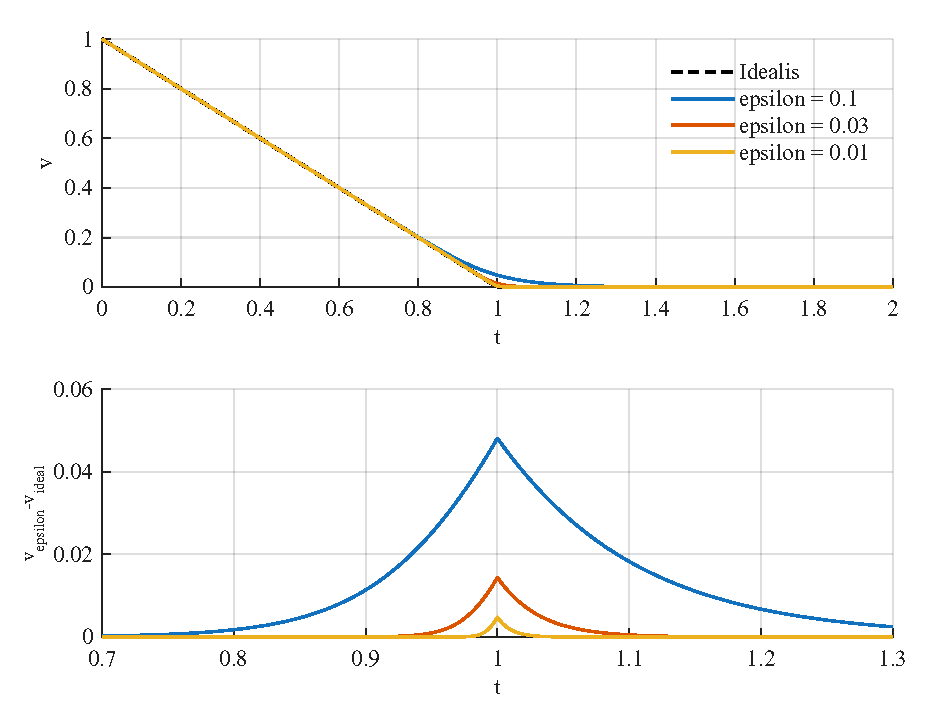
\includegraphics{graphics_v3/regularization_braking.pdf}
\caption{Lefékeződés külső erő nélkül, $v(0)=1$. Fent: az ideális és a három simított sebesség; lent: a sebességhiba a megállás környezetében. A simított görbék nullához tartanak, de nem érik el véges idő alatt.}\label{fig:regularization_braking}
\end{figure}
\exampleend

\subsection{Amikor félrevezet: tapadás helyett tartós kúszás}
\examplebody

Most ugyanarra az egységnyi tömegre hasson a súrlódási határnál kisebb, állandó $q=1/2$ erő, és induljunk nyugalomból: $x(0)=v(0)=0$. A kérdés az, hogy a test helyben marad-e. Az ideális modellben a statikus súrlódás kiegyenlíti az erőt, ezért $v(t)=0$, $x(t)=0$ minden időben. A simított modell más választ ad.

Az eltérés általános $q$ terhelésre is egyszerűen leírható. A dimenziótlan $m=F=1$, $0<q<1$ esetben az ideális statikus súrlódás $v=0$ mellett kiegyenlítheti a terhelést. A simított egyenlet viszont
\begin{equation}\label{eq:regularized_friction}
\dot v=q-\tanh(v/\varepsilon).
\end{equation}
A $v=0$ állapotban $\dot v=q>0$, tehát nincs pontos tapadás. Az egyetlen stacionárius sebesség
\begin{equation}\label{eq:creep_speed}
v_\varepsilon=\varepsilon\operatorname{artanh}(q),\qquad
\left.\frac{d\dot v}{dv}\right|_{v_\varepsilon}
=-\frac{1-q^2}{\varepsilon}<0.
\end{equation}
A sebesség stabil, de pozitív: a test lassan kúszik. $q=1/2$ mellett $v_\varepsilon\simeq0{,}549306\varepsilon$. Rögzített véges időn a kúszás hatása csökkenhet $\varepsilon$-nal, de hosszú idő alatt jelentős helyzethiba gyűlhet össze. A határerőhöz közeli $q\to1^-$ tartományban ez a becslés nem egyenletes.

A $q=1/2$, $\varepsilon=0{,}01$ példában a beálló sebesség mindössze $v_\varepsilon\simeq0{,}00549306$, de folyamatosan pozitív. A rövid kezdeti beállás után
\[
x_\varepsilon(t)\simeq0{,}00549306\,t,
\]
így $t=100$-nál már körülbelül $0{,}549$ a helyzeteltérés, míg az ideális test továbbra is az origóban áll. Az ODE pontosabb integrálása ezt nem szünteti meg: a kúszás a simított egyenlet megoldásának tulajdonsága.

Az $\varepsilon$ csökkentése a hibát lassabban felhalmozódóvá teszi, de véges $\varepsilon$ mellett nem állítja vissza a tapadást. Például $\varepsilon=0{,}001$ és $t=1000$ mellett közel ugyanekkora elmozdulást kapunk. Általánosan $t=1/\varepsilon$ időskálán $x_\varepsilon(t)\to\operatorname{artanh}(1/2)\simeq0{,}549306$, miközben az ideális elmozdulás nulla. A közelítés tehát rögzített véges időn javulhat, de tetszőlegesen hosszú időre nem ad egyenletesen kis helyzethibát.

Ha a feladat a tapadás fennmaradásának vagy a hosszú idejű helyzetnek a meghatározása, ez a simítás nem megfelelő modell. Ilyenkor külön tapadási módot használunk a $|q|\leq1$ erőfeltétellel, és csak a határ túllépésekor indítjuk el a mechanikai csúszást. A két példa különbsége az ellenőrzött mennyiségben is megmutatkozik: a kis sebességhiba még nem garantál kis, hosszú idejű helyzethibát.


A \ref{fig:regularization_creep}. ábrán felül a pozitív kúszósebesség gyors beállását, alul a hosszú idő alatt felhalmozódó elmozdulást látjuk. Az ideális megoldás mindkét panelen nulla. A két panel időtengelye eltér: a sebességnél $0\leq t\leq1$, a helyzetnél $0\leq t\leq100$ szerepel, hogy a gyors beállás és a lassú hibafelhalmozódás egyaránt látható legyen. A teljes kód az A függelék \ref{ap:regularization}. szakaszában található.
\begin{figure}[htbp]\centering
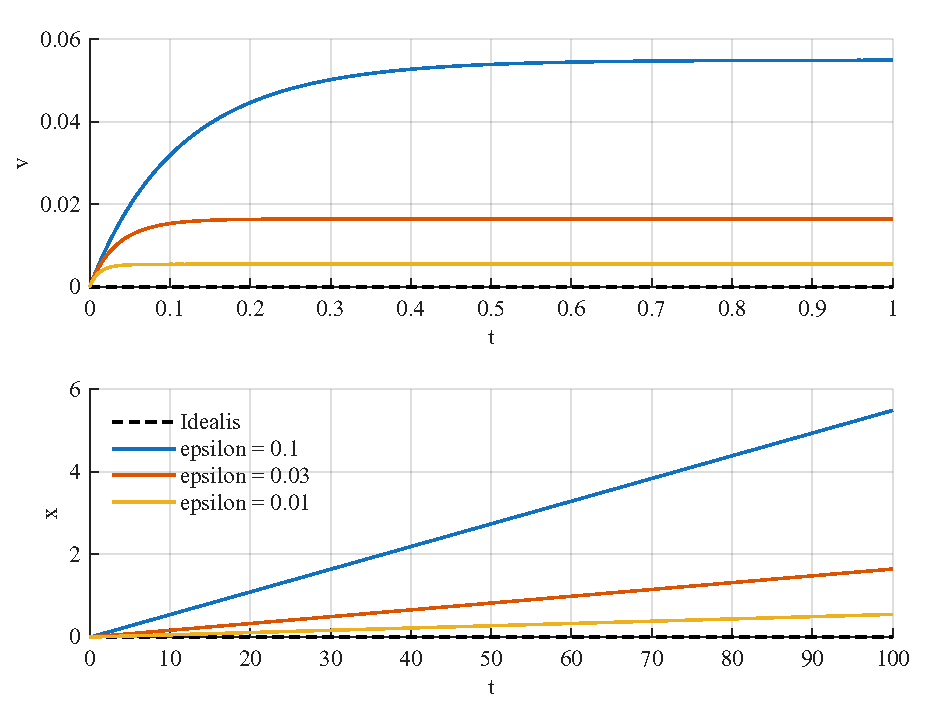
\includegraphics{graphics_v3/regularization_creep.pdf}
\caption{Tapadás helyett kúszás: $q=1/2$, $x(0)=v(0)=0$. Fent a sebesség, lent az elmozdulás összehasonlítása. A kisebb simítási szélesség kisebb sebességet ad, de véges $\varepsilon$ mellett az elmozdulás tovább növekszik.}\label{fig:regularization_creep}
\end{figure}

\begin{figure}[!htbp]\centering
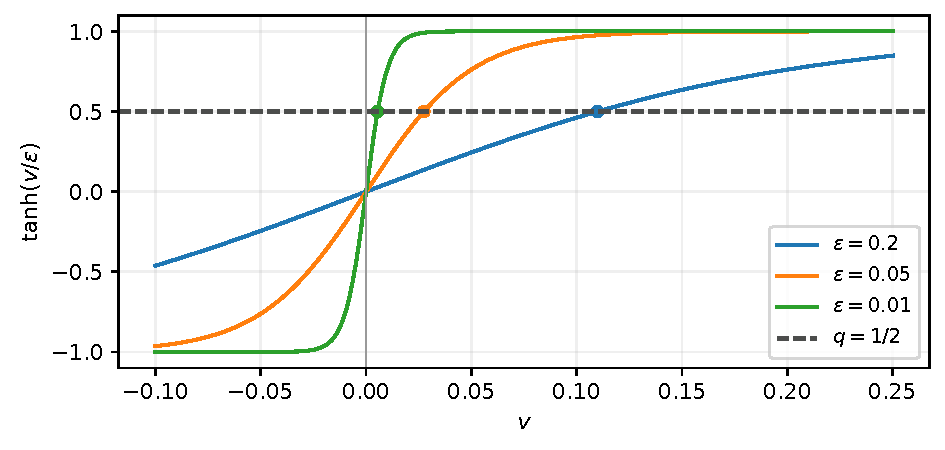
\includegraphics[width=\linewidth]{graphics_v3/friction_regularization.pdf}
\caption{Simított súrlódás $q=1/2$ mellett. A terhelés és a súrlódási görbe metszése pozitív kúszósebességet ad; az ideális tapadás sebessége nulla.}\label{fig:regularization_new}
\end{figure}
\phantomsection\label{use:regularization}A teljes MATLAB-program az A függelék \ref{ap:regularization}. szakaszában található (\pageref{ap:regularization}. oldal).

A kód a kis $\varepsilon$ mellett gyors relaxáció miatt \texttt{ode15s} megoldót használ. A relaxáció időskálája $\varepsilon/(1-q^2)$. Összetettebb modellben ez a lassú mechanikai időskálához képest numerikus merevséget okozhat. A simítás szélessége modellparaméter; a megoldó toleranciája ettől külön numerikus paraméter. Először rögzített $\varepsilon$ mellett kell numerikus konvergenciát vizsgálni, majd több $\varepsilon$ értékkel a modellérzékenységet.
\exampleend

\subsection{Merev fal helyett rugalmas kontaktus}
\examplebody

A másik gyakori közelítés az azonnali ütközés helyett rövid kontaktusfázis. Legyen $h$ a rés, $\delta=\max(0,-h)$ a benyomódás. A legegyszerűbb tisztán rugalmas büntetőmodell $N=K\delta$ nyomóerőt ad. A kontaktus közbeni kis behatolás ekkor a modell része, a kontaktus időskálája $\sqrt{m/K}$.

Külső erők nélkül a benyomódásra $m\ddot\delta+K\delta=0$ adódik. $\delta(0)=0$, $\dot\delta(0)=V>0$ mellett
\[
\delta(t)=\frac{V}{\sqrt{K/m}}\sin\!\left(\sqrt{K/m}\,t\right).
\]
Az első visszatérés ideje $t_c=\pi\sqrt{m/K}$, a maximális behatolás $V\sqrt{m/K}$. Kilépéskor a sebesség nagysága ismét $V$: ez $r=1$ visszapattanásnak felel meg. A nagyobb $K$ rövidebb kontaktust és kisebb behatolást ad, de \emph{önmagában nem hoz létre} $r<1$ energiaveszteséget. Ehhez disszipatív kontaktustörvény és elválási feltétel kell; az így kapott visszapattanási tényezőt a választott törvényből kell meghatározni.

Az ideális ütköző, a rugalmas kontaktus és a simított kapcsolás különböző modellek. Összevetésükkor az ütközési impulzust, a visszapattanási sebességet, a kontaktusidőt és a periódust érdemes ellenőrizni. Különösen grazing vagy tartós kontaktus közelében nem elegendő arra hivatkozni, hogy az átmenet keskeny vagy a rugó merev: a közelítés éppen a vizsgált helyi dinamikát változtathatja meg.
\exampleend

\section{Boundary equilibrium bifurcations}\label{sec:beb}
Egy paraméter változtatásakor az egyensúly elérheti a kapcsolófelületet. Ezt a helyzetet \emph{boundary equilibrium bifurcation} (BEB) néven tárgyalja \cite[5.1--5.2. szakasz]{dib}. Először a két oldali vektormező egyensúlyait külön számítjuk ki, majd ellenőrizzük, hogy a kapott gyök a megfelelő tartományban van-e. Az ilyen gyök \emph{admissible equilibrium}; a másik tartományba eső, formálisan folytatott gyök \emph{virtual equilibrium}. A kapcsolófelületen fekvő egyensúly \emph{boundary equilibrium}. A virtual equilibrium nem a teljes rendszer állandósult megoldása.

\subsection{Persistence: az egyensúly fennmarad}
\examplebody

Egy erősen csillapított, kétféle pozitív merevségű rugóval megtámasztott szerkezet dimenziótlan modellje legyen
\begin{equation}
 \dot x=\begin{cases}\mu-x,&x<0,\\ \mu-2x,&x\geq0.\end{cases}
 \label{eq:beb_persistence}
\end{equation}
Itt $x$ az elmozdulás, $\mu$ az állandó terhelés. A vektormező $x=0$-ban folytonos. A bal oldali egyensúlyjelölt $x_L=\mu$, a jobb oldali $x_R=\mu/2$. Ha $\mu<0$, csak $x_L$ admissible; ha $\mu>0$, csak $x_R$ admissible. A fizikai egyensúly tehát
\[
 x^*(\mu)=\begin{cases}\mu,&\mu\leq0,\\\mu/2,&\mu\geq0.\end{cases}
\]
Mindkét oldalon aszimptotikusan stabil, mert az állapot szerinti derivált rendre $-1$ és $-2$. A kritikus pontban is minden közeli pálya az origóhoz tart. Ezt az ággeometriát \emph{persistence} esetnek nevezzük: a megoldás átjut a kapcsolófelületen, de stabilitása itt nem változik. Az egyensúlyág meredekségének törése önmagában nem jelent új rezgésállapotot vagy stabilitásvesztést.
\exampleend

\subsection{Non-smooth fold: két egyensúly eltűnik}
\examplebody

A jobb oldalon aktív szabályozással negatív eredő merevséget is létrehozhatunk. Ennek legegyszerűbb helyi modellje
\begin{equation}
 \dot x=\begin{cases}\mu-x,&x<0,\\\mu+x,&x\geq0.\end{cases}
 \label{eq:beb_fold}
\end{equation}
Ez is folytonos $x=0$-ban. Ha $\mu<0$, az $x_L=\mu<0$ egyensúly stabil, az $x_R=-\mu>0$ egyensúly instabil. Ha $\mu>0$, mindkét jelölt virtual, ezért a teljes rendszernek nincs egyensúlya. A két admissible ág $\mu=0$-nál találkozik és eltűnik: ez a \emph{non-smooth fold}. A kritikus egyensúly balról vonzó, jobbról taszító, tehát kétoldali értelemben nem stabil. A pozitív oldali $+x$ tag nem passzív rugót, hanem destabilizáló visszacsatolást modellez. Az egyensúly megszűnése ebből a helyi modellből nem igazolja periodikus pálya létrejöttét.
\exampleend

\subsection{Filippov-példa: valódi egyensúlyból pseudo-equilibrium}
\examplebody

Legyen $H(x,y)=y$, és tekintsük az alábbi dimenziótlan, relés beavatkozást szemléltető modellt:
\begin{equation}
 F^+(x,y)=\begin{pmatrix}-x\\\mu-y\end{pmatrix}\quad(y>0),\qquad
 F^-(x,y)=\begin{pmatrix}-x\\1\end{pmatrix}\quad(y<0).
 \label{eq:beb_filippov}
\end{equation}
Az $x$ változó egy stabil belső állapot, $y$ a szabályozott eltérés. Negatív eltérésnél a beavatkozás állandó pozitív változási sebességet hoz létre; pozitív eltérésnél az eltérés $\mu$ felé relaxál. Ha $\mu>0$, a $(0,\mu)$ egyensúly admissible és stabil. A felületi normális komponensek $\mu$ és $1$, ezért ekkor nincs attracting sliding.

Ha $\mu<0$, a felső mező egyensúlya virtual lesz, viszont $\mu<0<1$ miatt a két mező a felület felé mutat. A Filippov-kombinációban
\[
 F_s=(1-\alpha)F^++\alpha F^-,\qquad
 \alpha=\frac{-\mu}{1-\mu}\in(0,1),\qquad F_s(x,0)=\begin{pmatrix}-x\\0\end{pmatrix}.
\]
Így $(0,0)$ stabil \emph{pseudo-equilibrium}: a sliding dinamika egyensúlya, jóllehet egyik oldali mező sem nulla ott. A felület vonzó, és azon $\dot x=-x$ biztosítja a tangenciális stabilitást. A $\mu=0$ kritikus pontban az admissible egyensúly a felületre ér; $\mu<0$ esetén a stabil állandósult állapot sliding formájában folytatódik. A konvex súly tartományának ellenőrzése lényeges: $\mu>0$ esetén a formális képlet nem ad megengedett sliding megoldást. A Filippov-féle BEB további eseteit \cite[5.2. szakasz]{dib} rendszerezi.

\begin{figure}[!htbp]\centering
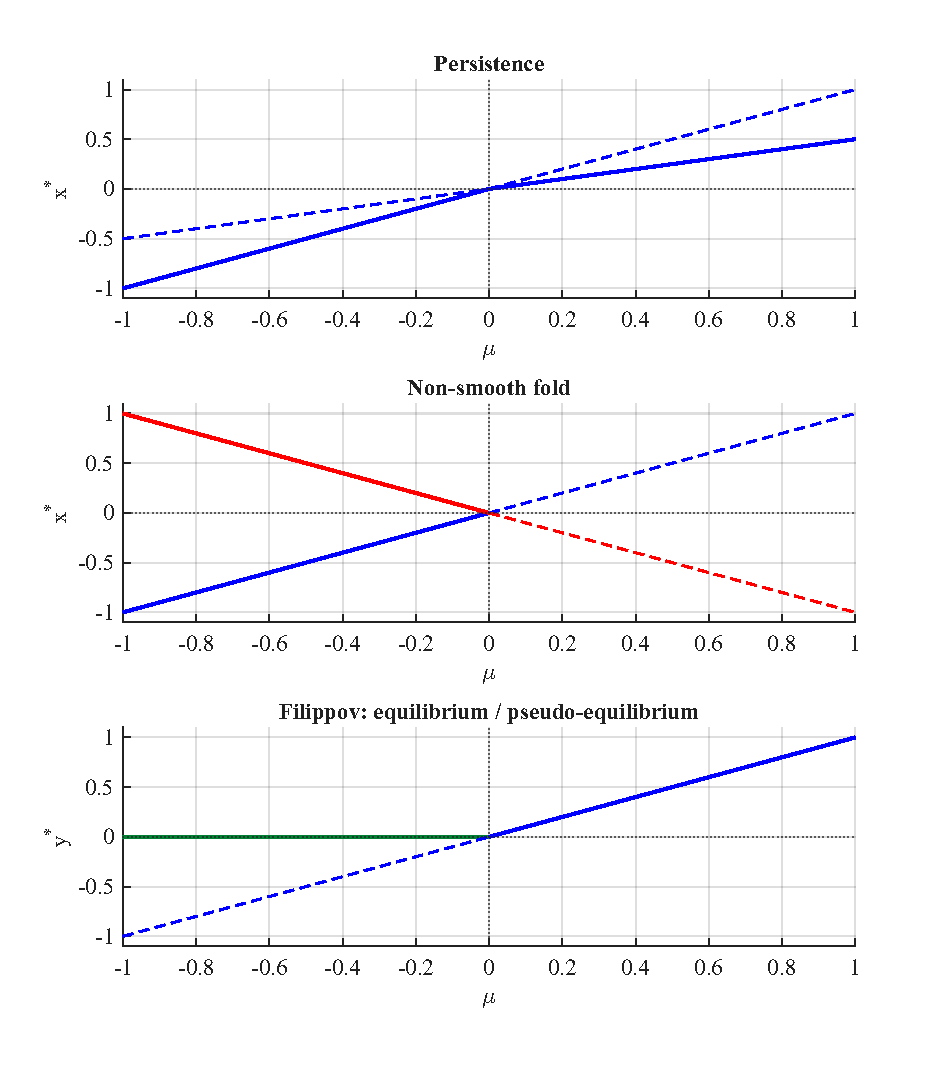
\includegraphics{graphics_v3/boundary_equilibria.pdf}
\caption{Három egyszerű BEB-példa. A folytonos vonal admissible, a szaggatott virtual ágat jelöl. A kék ág stabil, a piros instabil. Az alsó panelen a zöld ág stabil pseudo-equilibrium: a kapcsolófelületen folytatja a stabil állandósult állapotot. A színezés csak az admissible ágak fizikai stabilitását állítja.}\label{fig:beb_examples}
\end{figure}
\phantomsection\label{use:beb}A teljes ábrageneráló MATLAB-program az A függelék \ref{ap:beb}. szakaszában található.
\exampleend

\section{A sliding bifurcations négy helyi típusa}\label{sec:four_sliding}
A kapcsolófelület elérése és a sliding region határának elérése eltérő esemény. Az utóbbinál valamelyik oldali mező normális komponense nulla. A négy alaphelyzetet \cite[8.1. szakasz]{dib} tárgyalja; relés szabályozási alkalmazást a könyv 8.2. szakasza ad. Az alábbi dimenziótlan modellek a helyi pályageometriát szemléltetik. A pályacsalád változtatása önmagában még nem periodikus pálya bifurkációja: ehhez olyan globális visszatérés is kell, amely a pályát újra ebbe a környezetbe vezeti.

\subsection{Crossing--sliding}
\examplebody

Legyen $H(x,y)=y$, felül $F^+=(1,x)^T$, alul $F^-=(1,1)^T$. A $y=0$, $x<0$ félegyenes attracting sliding region, mert a normális komponensek $x<0<1$. Mindkét mező első komponense egy, ezért a sliding mozgás $\dot x=1$, $\dot y=0$. A pálya a határon, $x=0$-nál a felső tartományba lép ki.

Érkezzen egy alsó pálya a felület $(s,0)$ pontjába. Ha $s>0$, áthalad a felületen, majd a felső pálya $y=(x^2-s^2)/2$. Ha $s<0$, előbb sliding mozgással halad az $s\leq x\leq0$ szakaszon, és csak ezután követi a $y=x^2/2$ parabolát. Az $s=0$ kritikus esetben az érkező mező normális sebessége továbbra is $1$: az érkezés nem grazing. A változás a rövid sliding szakasz megjelenése. Mérnöki értelemben egy relés átkapcsolás után itt kezdődhet tartós, ideális sliding üzem.
\exampleend

\subsection{Grazing--sliding}
\examplebody

Ugyanebben a mezőben most a felső tartományból érkezzünk a $y=x^2/2+c$ pályán. Ha $c>0$, a pálya nem éri el a felületet. Ha $c=0$, az origóban érinti, és $\dot y=0$, $\ddot y=1$: ez nemelfajuló grazing. Ha $c<0$, az első találkozás $x=-\sqrt{-2c}$-nél történik, majd a pálya sliding mozgással jut az origóba. A sliding szakasz hossza $\sqrt{-2c}$. Itt tehát egy addig kapcsolásmentes mozgás válik sliding szakaszt tartalmazóvá. Száraz súrlódásnál ez egy új tapadási szakasz megjelenésének helyi modellje lehet; az adott súrlódási rendszerben a normális irányt a relatív sebesség határozza meg.
\exampleend

\subsection{Switching--sliding}
\examplebody

Most legyen $F^+=(1,-x)^T$, $F^-=(1,1)^T$. Az attracting sliding region $x>0$, és rajta továbbra is $\dot x=1$: a sliding mozgás a határtól távolodik. Egy alsó pálya ismét $(s,0)$-ban érkezzen. Ha $s>0$, azonnal sliding indul. Ha $s<0$, a pálya előbb a felső tartományba lép, ahol
\[
 y=\frac{s^2-x^2}{2},\qquad s\leq x\leq-s,
\]
majd $x=-s>0$-nél újra eléri a felületet és sliding mozgásra vált. Mindkét esetben van sliding, de az egyikben ezt rövid szabad mozgási szakasz előzi meg. A lényeg a kapcsolási sorrend megváltozása, nem az első sliding szakasz létrejötte.
\exampleend

\subsection{Adding--sliding}
\examplebody

A sliding pálya magának a sliding regionnak a határát is érintheti. Ennek természetes geometriájához két tangenciális koordinátát használunk. Legyen az állapot $(s,z,y)$, $H=y$, továbbá
\begin{equation}
 F^+=\begin{pmatrix}1\\0\\z-s^2\end{pmatrix},\qquad
 F^-=\begin{pmatrix}1\\0\\1\end{pmatrix}.
 \label{eq:adding_local}
\end{equation}
Az attracting sliding region $y=0$, $z<s^2$; a sliding mozgás $\dot s=1$, $\dot z=0$. A $z=\mu$ szinten haladó családban $\mu<0$ esetén megszakítás nélküli sliding zajlik. A $\mu=0$ pálya az origóban érinti a sliding region parabola alakú határát. Ha $\mu>0$, a pálya $s=-\sqrt\mu$-nél elhagyja a felületet. A szabad szakaszon
\begin{equation}
 y(s)=\mu s-\frac{s^3}{3}+\frac23\mu^{3/2},\qquad
 -\sqrt\mu\leq s\leq2\sqrt\mu.
\end{equation}
Ezt a $dy/ds=\mu-s^2$ egyenlet integrálásával, $y(-\sqrt\mu)=0$ feltétellel kapjuk. A visszaérkezés $s=2\sqrt\mu$-nél történik; ott $F_y^+=-3\mu<0$, így ismét sliding indul. Egy korábbi sliding intervallum helyén két sliding intervallum és köztük egy szabad kitérés jelenik meg. A maximális eltérés $4\mu^{3/2}/3$. Itt $\mu$ a pályacsalád állandó $z$ koordinátája; egy teljes rendszerben a globális dinamika határozná meg, hogyan függ ez a fizikai vezérlőparamétertől. Relés szabályozásnál ez egy rövid kilépés lehet a sliding üzemből.

\begin{figure}[!htbp]\centering
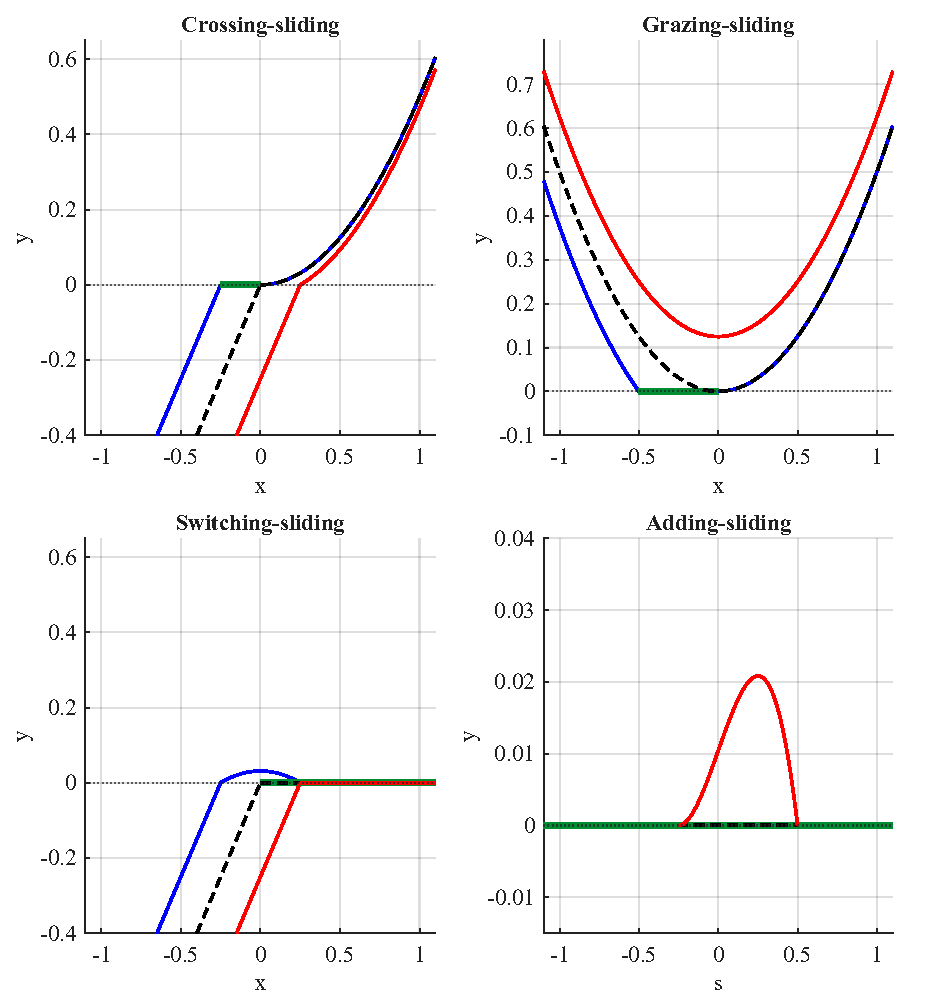
\includegraphics{graphics_v3/sliding_geometries.pdf}
\caption{A négy sliding geometria egzakt helyi pályákon. A kék, fekete szaggatott és piros görbe a kritikus helyzet két oldalát, illetve a kritikus pályát mutatja; a vastag zöld részek sliding szakaszok. Az adding--sliding panel a háromdimenziós pályák $(s,y)$ vetülete, így a megszakítás nélküli sliding pályák egymásra vetülnek. Minden panelen balról jobbra halad az idő.}\label{fig:four_sliding}
\end{figure}
\phantomsection\label{use:sliding_types}Az egzakt pályákat kirajzoló teljes MATLAB-kód az A függelék \ref{ap:sliding_types}. szakaszában szerepel.
\exampleend

\section{Grazing folytonos piecewise-smooth rendszerben}\label{sec:continuous_grazing}
Az ütközéses rendszer grazing leképezésének square-root tagját nem szabad automatikusan átvinni egy folytonos vektormezőre. Ha a kapcsolófelületen maga a vektormező folytonos, de a deriváltja ugrik, a nemelfajuló grazing tipikus helyi korrekciója $3/2$ rendű. Ennek feltételeit és a discontinuity mapping levezetését \cite[7.2. szakasz, különösen 7.1. tétel]{dib} adja meg.

\subsection{Egyszerű mechanikai modell: egyoldali rugó}
\examplebody

Egy $m$ tömegre a kontaktustól elfelé ható állandó $ma$ erő működik, ahol $a>0$. A rés legyen $h$, sebessége $v$; a $h<0$ tartományban egy $k$ merevségű rugó kapcsolódik be. A modell
\begin{equation}
 \dot h=v,\qquad \dot v=a-\kappa\min(h,0),\qquad \kappa=k/m>0.
 \label{eq:continuous_contact}
\end{equation}
A negatív $h$ itt rugalmas benyomódás, a modell megengedett állapota. Nincs sebességugrás vagy reset. A mező $h=0$-ban folytonos, Jacobi-mátrixa viszont a két oldalon
\[
 A_+=\begin{pmatrix}0&1\\0&0\end{pmatrix},\qquad
 A_-=\begin{pmatrix}0&1\\-\kappa&0\end{pmatrix}.
\]
A grazing állapot $(h,v)=(0,0)$: ott $\dot h=0$, de $\ddot h=a>0$.


A rugó nélküli referencia $h_0(t)=-\varepsilon+at^2/2$, ahol $\varepsilon>0$ a referencia behatolási mélysége. A belépési sebesség nagysága $V=\sqrt{2a\varepsilon}$, a referencia két felületi metszése közti idő $T_0=2V/a$. A belépéstől mért $\tau$ idővel a valódi kontaktuspálya
\begin{equation}
 h_c(\tau)=\frac a\kappa(1-\cos\sqrt\kappa\tau)
 -\frac V{\sqrt\kappa}\sin\sqrt\kappa\tau.
\end{equation}
Az első pozitív zérus és a hozzá tartozó sebesség
\[
 T_c=\frac2{\sqrt\kappa}\arctan\frac{V\sqrt\kappa}{a},\qquad v_c(T_c)=V.
\]
A két kilépési sebesség egyaránt $V$, de a kilépés időpontja eltér! Ezért az állapotokat közös időre kell hozni. A valódi pálya hamarabb hagyja el a kontaktust, majd $d=T_0-T_c>0$ ideig ismét $\dot v=a$ szerint mozog. A referencia kilépési időpontjában a különbség pontosan
\begin{equation}
 \Delta v=ad,\qquad \Delta h=Vd+\frac12ad^2.
 \label{eq:continuous_grazing_exact}
\end{equation}
Az $\arctan u=u-u^3/3+O(u^5)$ sorfejtést behelyettesítve
\begin{equation}
 \Delta v=\frac{4\kappa}{3}\sqrt{\frac2a}\,\varepsilon^{3/2}
 +O(\varepsilon^{5/2}),\qquad
 \Delta h=\frac{8\kappa}{3a}\varepsilon^2+O(\varepsilon^3).
 \label{eq:continuous_grazing_order}
\end{equation}
Az esemény időtartama $O(\sqrt\varepsilon)$, de ezalatt a két mező gyorsuláskülönbsége csak $O(\varepsilon)$. Szorzatuk adja a vezető $O(\varepsilon^{3/2})$ sebességkorrekciót. A pozíciókomponens ebben a modellben még magasabb rendű. A vezető tag együtthatójának dimenziója is helyes: $[\kappa]=\mathrm{s}^{-2}$ és $[a]=\mathrm{m}\,\mathrm{s}^{-2}$ mellett $\kappa a^{-1/2}\varepsilon^{3/2}$ sebesség.

Ha a referencia nem hatol be, nincs kontaktuskorrekció. Ezért a paraméterfüggésben egyoldali $[\varepsilon]_+^{3/2}$ jellegű tag jelenik meg. Ennek első deriváltja a kritikus pontban nulla, míg második deriváltja a pozitív oldalról korlátlan. Ez lényegesen enyhébb szingularitás, mint a merev ütközésnél fellépő square-root tag. Az eredmény rögzített véges $\kappa$ és kis $\varepsilon$ mellett érvényes; a $\kappa\to\infty$ merev kontaktushatár nem helyettesíthető be ebbe a sorfejtésbe. Periodikus pálya bifurkációjának megállapításához itt is szükséges a teljes visszatérési leképezés.

\begin{figure}[!htbp]\centering
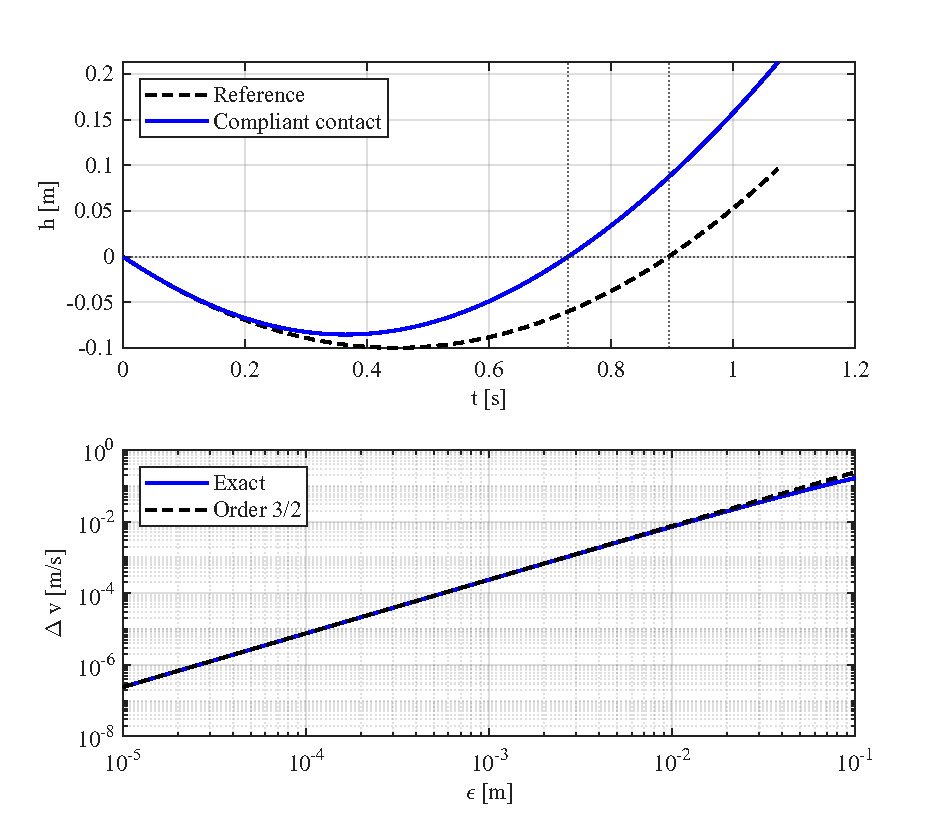
\includegraphics{graphics_v3/continuous_grazing.pdf}
\caption{Folytonos kontaktusmodell, $a=1\,\mathrm{m/s^2}$, $\kappa=4\,\mathrm{s^{-2}}$. Felül a referencia és a rugós pálya résfüggvénye $\varepsilon=0.1\,\mathrm m$ esetén; az idő a belépéstől indul. A rugó csökkenti a benyomódást és előrehozza a kilépést. Alul az azonos időpontban mért egzakt sebességkorrekció és annak $3/2$ rendű közelítése logaritmikus tengelyeken.}\label{fig:continuous_grazing}
\end{figure}
\FloatBarrier
\phantomsection\label{use:continuous_grazing}A teljes MATLAB-program az A függelék \ref{ap:continuous_grazing}. szakaszában található; az egzakt megoldást és a rendbecslést is kiértékeli.
\exampleend


\begin{thebibliography}{99}
\addcontentsline{toc}{chapter}{Irodalomjegyzék}
\bibitem{dib} M. di Bernardo, C. J. Budd, A. R. Champneys, P. Kowalczyk: \emph{Piecewise-smooth Dynamical Systems: Theory and Applications}. Springer, 2008. \url{https://doi.org/10.1007/978-1-84628-708-4}.
\bibitem{kuznetsov_book} Y. A. Kuznetsov: \emph{Elements of Applied Bifurcation Theory}. 3. kiadás, Applied Mathematical Sciences 112, Springer, 2004. \url{https://doi.org/10.1007/978-1-4757-3978-7}.
\bibitem{kuznetsov} Y. A. Kuznetsov: Andronov--Hopf bifurcation. \emph{Scholarpedia}, 1(10):1858, 2006. \url{https://doi.org/10.4249/scholarpedia.1858}.
\bibitem{kong} N. J. Kong, J. J. Payne, J. Zhu, A. M. Johnson: Saltation Matrices: The Essential Tool for Linearizing Hybrid Dynamical Systems. 2024-es átdolgozás. \url{https://arxiv.org/abs/2306.06862v3}.
\bibitem{nordmark} A. B. Nordmark: Non-periodic motion caused by grazing incidence in an impact oscillator. \emph{Journal of Sound and Vibration}, 145(2), 279--297, 1991. \url{https://doi.org/10.1016/0022-460X(91)90592-8}.
\bibitem{auto} E. J. Doedel és az AUTO-07p fejlesztői: \emph{AUTO-07p: Continuation and Bifurcation Software for Ordinary Differential Equations}. Kézikönyv és forráskód. \url{https://github.com/auto-07p/auto-07p/tree/master/doc}.
\bibitem{geyer} H. Geyer, A. Seyfarth, R. Blickhan: Spring-mass running: simple approximate solution and application to gait stability. \emph{Journal of Theoretical Biology}, 232, 315--328, 2005. \url{https://doi.org/10.1016/j.jtbi.2004.08.015}.

\bibitem{matlab_events} MathWorks: \emph{ODE Event Location}. MATLAB dokumentáció. \url{https://www.mathworks.com/help/matlab/math/ode-event-location.html}. Hozzáférés: 2026. október 28.
\bibitem{champneys_dib} A. R. Champneys, M. di Bernardo: Piecewise smooth dynamical systems. \emph{Scholarpedia}, 3(9):4041, 2008. \url{https://doi.org/10.4249/scholarpedia.4041}.
\bibitem{or_teel} Y. Or, A. R. Teel: Using the Set-Valued Bouncing Ball for Bounding Zeno Solutions of Lagrangian Hybrid Systems. \emph{IFAC Proceedings Volumes}, 43(14), 801--806, 2010. \url{https://doi.org/10.3182/20100901-3-IT-2016.00128}.
\bibitem{goebel_sanfelice} R. Goebel, R. G. Sanfelice: How Well-Posedness of Hybrid Systems Can Extend Beyond Zeno Times. \emph{IEEE Conference on Decision and Control}, 2016. \url{https://doi.org/10.1109/CDC.2016.7798334}.
\bibitem{sotomayor_teixeira} J. Sotomayor, M. A. Teixeira: \emph{Regularization of Discontinuous Vector Fields}. 1996. Szerzői kézirat, Universidade de São Paulo repozitóriuma. \url{https://repositorio.usp.br/bitstreams/5bcd7c7a-0f9e-40eb-a527-37899bff717d}.
\end{thebibliography}

\appendix
\chapter{Numerikus példák és ellenőrzések}\label{ap:all_codes}
\lstset{basicstyle=\ttfamily\fontsize{8.5}{10}\selectfont}
A jegyzet összes MATLAB-példaprogramja és a hozzájuk tartozó segédfüggvények a projekt \texttt{codes} könyvtárában találhatók. A \texttt{Contents.m} tartalomjegyzéket, a \texttt{README.txt} futtatási útmutatót ad; futtatás előtt ezt a könyvtárat az útvonalhoz kell adni. A peremfeladatokhoz \texttt{bvp5c}, a generikus korrektorhoz \texttt{fsolve} (Optimization Toolbox) szükséges. A példakódok az algoritmus lépéseire szorítkoznak; a bemenetek feltételeit a megjegyzések adják meg. Futás közben csak a konvergencia, a fizikai megoldáság és a szinguláris események miatt szükséges ellenőrzések maradtak meg. Az adott paramétertartomány konvergenciavizsgálatát külön kell elvégezni.
\paragraph*{Ábrák és automatikus ellenőrzések.}
A \texttt{codes/square\_root\_figures\_v3.py} program NumPy és PGFPlots használatával öt vektoros PDF-ábrát készít. A bifurkációs ábrák 241 paraméterértéket, 2320 tranziens iterációt és 80 megtartott iterátumot használnak, minden pontban $w_0=0$ kezdeti értékkel. A cobweb diagramok 24 iterációt mutatnak.

A \texttt{checks/verify\_p1.py} a P1-es mátrixokat és invariánsokat, a \texttt{checks/verify\_p23.py} a folytatást, a vetítést, a grazing-geometriát, az admissibility feltételeit és a forráshivatkozásokat ellenőrzi. A Python-ellenőrzések nem futtatják a MATLAB-megoldókat; utóbbiakat a célrendszeren külön is ellenőrizni kell.

A főszöveg példái az alábbi teljes kódlistákra hivatkoznak. Minden program egyszer szerepel; a szakaszok elején visszahivatkozás mutat az alkalmazás helyére.

\clearpage
\section{Határciklus monodrómia-mátrixa}\label{ap:monodromy}
Alkalmazás és magyarázat a főszöveg \pageref{use:monodromy}. oldalán. 
Fájl: \path{codes/Monodromia_mx_pelda_v3.m}.
\lstinputlisting[caption={Határciklus monodrómia-mátrixa},label={lst:monodromy}]{codes/Monodromia_mx_pelda_v3.m}

\clearpage
\section{Harmonikus oszcillátor negyedperiódus-feladata}\label{ap:spring_bvp}
Alkalmazás és magyarázat a főszöveg \pageref{use:spring_bvp}. oldalán. 
Fájl: \path{codes/mass_spring_bvp_v3.m}.
\lstinputlisting[caption={Harmonikus oszcillátor negyedperiódus-feladata},label={lst:spring_bvp}]{codes/mass_spring_bvp_v3.m}

\clearpage
\section{Ütközéses állapot- és variációs integrálás}\label{ap:codes1}
Fájl: \path{codes/impact_monodromy_v3.m}.
A függvény az állapotot és a variációs mátrixot együtt integrálja, az ütközéseknél saltation-korrekcióval. Általános kezdeti állapotnál a visszaadott mátrix a véges idejű leképezés deriváltja; csak periodikus pályán monodrómia-mátrix. Alkalmazását a \ref{sec:square_root}. fejezet tárgyalja. Példahívás:
\begin{lstlisting}[numbers=none]
[yT,M,t,y,nImpact] = impact_monodromy_v3([1;0],0,2*pi/3,0.05,3,0.8,0);
\end{lstlisting}
\lstinputlisting[caption={Ütközéses állapot- és variációs integrálás},label={lst:codes1}]{codes/impact_monodromy_v3.m}

\clearpage
\section{Generikus pseudo-arclength korrektor}\label{ap:pal}
Fájl: \path{codes/pal_corrector_v3.m}.
A korrektorhoz \texttt{fsolve} szükséges. A \ref{ap:fold}. szakasz teljes példája mutatja a használatát.
\lstinputlisting[caption={Generikus pseudo-arclength korrektor},label={lst:pal}]{codes/pal_corrector_v3.m}

\clearpage
\section{Áthaladás egy visszahajláson}\label{ap:fold}
Alkalmazás és magyarázat a főszöveg \pageref{use:fold}. oldalán. 
Fájl: \path{codes/fold_pal_v3.m}.
A program a \ref{ap:pal}. szakaszban közölt korrektorra támaszkodik; mindkét fájl legyen a MATLAB útvonalán.
\lstinputlisting[caption={Áthaladás egy visszahajláson},label={lst:fold}]{codes/fold_pal_v3.m}

\clearpage
\section{Feldobás peremérték-feladata}\label{ap:apex_bvp}
Alkalmazás és magyarázat a főszöveg \pageref{use:apex_bvp}. oldalán. 
Fájl: \path{codes/apex_bvp_v3.m}.
\lstinputlisting[caption={Feldobás peremérték-feladata},label={lst:apex_bvp}]{codes/apex_bvp_v3.m}

\clearpage
\section{Feldobás shooting módszerrel}\label{ap:apex_shooting}
Alkalmazás és magyarázat a főszöveg \pageref{use:apex_shooting}. oldalán. 
Fájl: \path{codes/apex_shooting_v3.m}.
\lstinputlisting[caption={Feldobás shooting módszerrel},label={lst:apex_shooting}]{codes/apex_shooting_v3.m}

\clearpage
\section{Tömeg--rugó rendszer paraméterkövetése}\label{ap:spring_cont}
Alkalmazás és magyarázat a főszöveg \pageref{use:spring_cont}. oldalán. 
Fájl: \path{codes/spring_continuation_v3.m}.
\lstinputlisting[caption={Tömeg--rugó rendszer paraméterkövetése},label={lst:spring_cont}]{codes/spring_continuation_v3.m}

\clearpage
\section{Kétféle merevségű rugó: illesztett peremfeladat}\label{ap:bilinear}
Alkalmazás és magyarázat a főszöveg \pageref{use:bilinear}. oldalán. 
Fájl: \path{codes/bilinear_bvp_v3.m}.
\lstinputlisting[caption={Kétféle merevségű rugó: illesztett peremfeladat},label={lst:bilinear}]{codes/bilinear_bvp_v3.m}

\clearpage
\section{Pattogó labda eseményvezérelt integrálása}\label{ap:ball}
Alkalmazás és magyarázat a főszöveg \pageref{use:ball}. oldalán. 
Fájl: \path{codes/bouncing_ball_v3.m}.
\lstinputlisting[caption={Pattogó labda eseményvezérelt integrálása},label={lst:ball}]{codes/bouncing_ball_v3.m}

\clearpage
\section{Stick--slip egzakt szakaszokkal}\label{ap:stick}
Alkalmazás és magyarázat a főszöveg \pageref{use:stick}. oldalán. 
Fájl: \path{codes/stick_slip_v3.m}.
\lstinputlisting[caption={Stick--slip egzakt szakaszokkal},label={lst:stick}]{codes/stick_slip_v3.m}

\clearpage
\section{Border-collision bifurcation egy szakaszonként lineáris leképezésben}\label{ap:border}
Alkalmazás és magyarázat a főszöveg \pageref{use:border}. oldalán. 
Fájl: \path{codes/border_collision_v3.m}.
\lstinputlisting[caption={Border-collision bifurcation egy szakaszonként lineáris leképezésben},label={lst:border}]{codes/border_collision_v3.m}

\clearpage
\section{Súrlódási modell regularizálása}\label{ap:regularization}
Alkalmazás és magyarázat a főszöveg \pageref{use:regularization}. oldalán. 
Fájl: \path{codes/friction_regularization_v3.m}. Indítás: \lstinline|friction_regularization_v3|. A teljes program mindkét regularizációs példát numerikusan megoldja, analitikus ellenőrzést végez, majd a két összehasonlító ábrát PDF- és SVG-formátumban elmenti. Minden segédfüggvény ugyanebben a fájlban szerepel.
\lstinputlisting[caption={Súrlódási modell regularizálása},label={lst:regularization}]{codes/friction_regularization_v3.m}

\clearpage
\section{Boundary equilibrium bifurcations}\label{ap:beb}
Alkalmazás a főszöveg \pageref{use:beb}. oldalán. A program önállóan futtatható; PDF- és SVG-ábrát készít.
\lstinputlisting[caption={Boundary equilibrium bifurcations}]{codes/boundary_equilibria_v3.m}

\clearpage
\section{A négy sliding geometria}\label{ap:sliding_types}
Alkalmazás a főszöveg \pageref{use:sliding_types}. oldalán. A program önállóan futtatható; PDF- és SVG-ábrát készít.
\lstinputlisting[caption={A négy sliding geometria}]{codes/sliding_geometries_v3.m}

\clearpage
\section{Grazing folytonos kontaktusmodellben}\label{ap:continuous_grazing}
Alkalmazás a főszöveg \pageref{use:continuous_grazing}. oldalán. A program önállóan futtatható; PDF- és SVG-ábrát készít.
\lstinputlisting[caption={Grazing folytonos kontaktusmodellben}]{codes/continuous_grazing_v3.m}

\clearpage
\section{További programok és ábragenerátorok}
A SLIP-peremfeladat további alkalmazásként szerepel a \texttt{codes} könyvtárban. A SLIP-kód bemenete közös $[0,1]$ rács, nyolckomponensű pályabecslés, két időtartam és a fizikai paraméterstruktúra; nem bemenet nélküli demó.
A \path{codes/practical_figures_v3.py} a \ref{sec:practical}. fejezet egzakt referenciaábráit állítja elő. A további ábragenerátorokat és futtatásukat a \path{codes/README.txt} sorolja fel.

\end{document}
